\setchapterstyle{kao}
\setchapterpreamble[u]{\margintoc}

\chapter{Detecting Low Energy Double Cascades}
\labch{double_cascade_performance}


\section{Reconstruction} \labsec{dc_reconstruction}

All existing reconstruction algorithms applied for low energy atmospheric neutrino events mentioned in \refsec{reconstruction} are either assuming a single cascade hypothesis or a track and cascade hypothesis, which are the two SM morphologies observable at these energies, as was described in \refsec{icecube_signatures}. A HNL being produced and decaying inside the IceCube detector however, will produce two cascade like light depositions. The morphology, spatial separation between the cascades, and their individual properties depend on the model parameters discussed in \refsec{double_cascade_morphology}. To investigate the performance of the detector to observe and identify these events, a low energy double cascade reconstruction algorithm was developed. It is based on a pre-existing algorithm used to search for double cascades produced from high energy astrophysical tau neutrinos \sidecite{Abbasi:2020zmr} that was established in \sidecite{MUsner}, but first mentioned in \sidecite{PHallen}.


\subsection{Table-Based Minimum Likelihood Algorithms}

The aforementioned reconstruction is relying on a minimum likelihood algorithm, which is the \textit{classical} approach to IceCube event reconstructions, as opposed to ML based methods. It compares the observed light depositions in the detector to the expected light depositions from a given event hypothesis, where the event hypothesis can be constructed from building blocks of single cascade and track segment expectations. Varying the energies of the track segments and cascade components, will change the expected light and can be used to find the best fit to the observed light. A Poissonian likelihood is constructed, which compares the observed photon numbers, $n$, with their arrival times to the expected light depositions, $\mu$, for a given even hypothesis as
% \todo{maybe I want a figure for this, or not so important? (YELLOW)}
\begin{equation}
    \ln(L) = \sum_j \sum_t n_{j,t} \cdot \ln(\mu_{j,t}(\Theta) + \rho_{j,t}) - (\mu_{j,t}(\Theta) + \rho_{j,t}) - \ln(n_{j,t}!)
    \;,
    \labeq{millipede_likelihood}
\end{equation}
where $\rho$ are the number of expected photons from noise, $\Theta$ are the parameters governing the source hypothesis, and the likelihood is calculated summing over all DOMs $j$ splitting observed photons into time bins $t$. The light expectations are calculated using look-up tables \sidecite{photospline} that contain the results from MC simulations of cascade events or track segments. By varying the parameters defining the event hypothesis, the likelihood of describing the observed light pattern by the expected light depositions is minimized to find the reconstructed event. Algorithms of this kind used in IceCube are described in great detail in \sidecite{IceCube:2013dkx}. For the table production a specific choice of ice model has to be made, while the calibrated DOM information is taken from the measurement itself.

% \subsection{Double Cascade Hypothesis}

Based on the tabulated light expectations for cascades and track segments, various event hypothesis can be constructed, like the common cascade only or the track and cascade hypotheses. The hypothesis describing the double cascade signature of the HNL is using two cascades that are separated by a certain distance. The whole hypothesis is defined by 9 parameters and assumes that the two cascades are aligned with each other, which is a safe assumption for strongly forward boosted interactions. The parameters are the position of the first cascade, $x, y, z$, the direction of both cascades, $\phi, \theta$, and its time, $t$, as well as the decay length, $L$, between the two cascades. Assuming the speed of the HNL to be the speed of light, $c$, this already defines the full hypothesis, because the time and position of the second cascade are then fully determined by properties of the first cascade and the decay length. Note here, that the HNL particle does not produce any light while traveling, as it is electrically neutral. Since the likelihood only sums over DOMs that have observed photons, the non-observation of light is used as information and will exclude hypotheses with light expectation in those DOMs. The full 9 parameters describing the event are $\Theta = (x, y, z, t, \theta, \phi, E_0, E_1, L)$. To compute the full likelihood, the term in \refeq{millipede_likelihood} defined for a single event hypothesis, is summed over both cascade contributions, as $\sum_i \ln(L_i)$, with $i$ being the cascade index.


\subsection{Optimization for Low Energies}

Optimizing the double cascade reconstruction for low energy events was done in parallel to the development of the model dependent simulation generator introduced in \refsec{model_specific_simulation}. A preliminary sample of HNL events from the model dependent simulation was used, containing a continuum of masses between \SIrange[range-phrase=~and~]{0.1}{1.0}{\gev} and lab frame decay lengths sampled uniformly in the range from \SIrange{5}{500}{\meter}. Even though this sample is not representative of a physically correct model and therefore not useful to predict the event expectation, it can still be used to optimize the reconstruction. The double cascade nature of the individual events and the evenly spaced decay length distribution are especially useful for this purpose.

The simulation is processed up to Level 5 of the selection chain described in \refsec{event_selection} and one of the reconstructions from \sidecite{low_energy_reco_IC} is applied to the events, fitting a cascade and a track and cascade hypothesis. The results from this reconstruction are used as an input for the double cascade reconstruction, where the position of the vertex, the direction of the event, and its interaction time are used as the input quantities for the first cascade, and the length of the track reconstruction is used as a seed for the distance between the two cascades.


\subsubsection{Decay Length Seeds}

\begin{marginfigure}
	\centering
    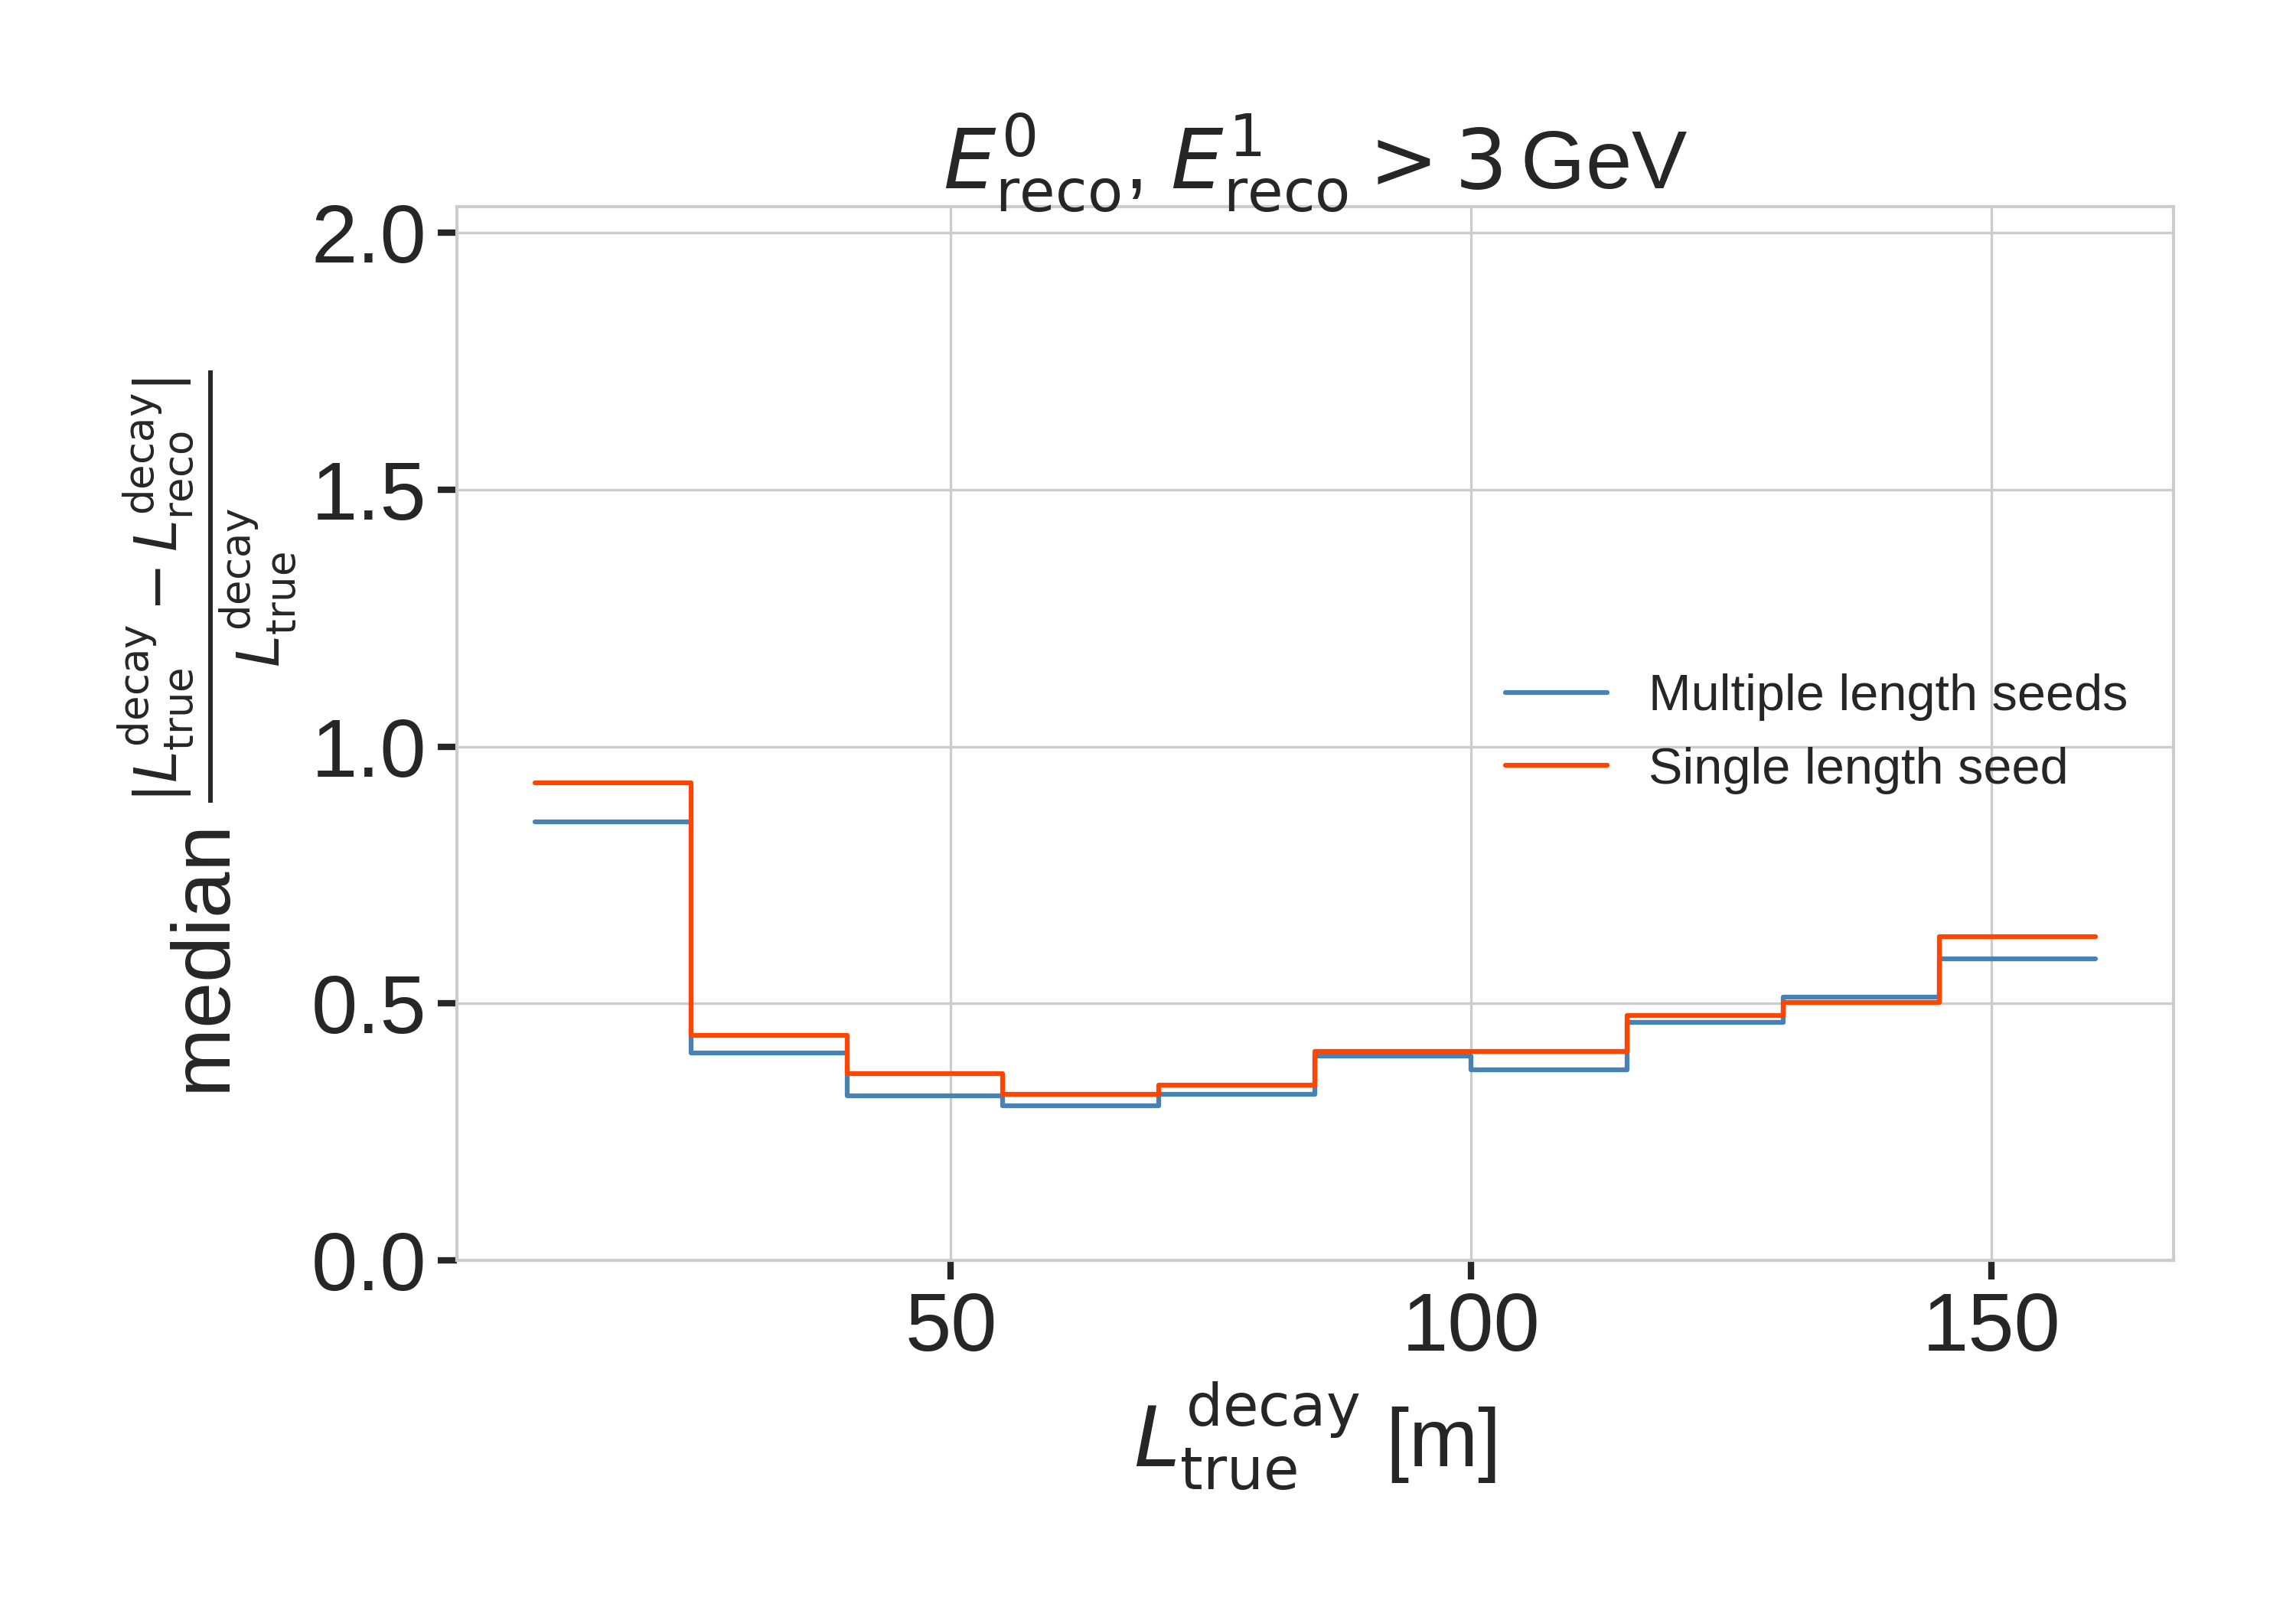
\includegraphics{figures/results/190605_reco_optimization/decay_length_seeding_median_decay_length_resolution_Good + L7 + reco E1,E2 above 3_fix_y.png}
    \caption[Decay length resolutions to optimize length seeding]{Decay length resolution as a function of the true decay length, comparing the same fit routine seeded with just the seed decay length and seeded with a decay length of \SI{5}{\meter}, \SI{25}{\meter}, \SI{50}{\meter}, \SI{100}{\meter}, and \SI{200}{\meter} on the left. Only events that had more than \SI{3}{\gev} in both cascades are used, and the resolutions are unweighted.}
    \labfig{fit_routine_optimization_decay_length_seeding}
\end{marginfigure}
\todo{Remake with better dimensions, so it fits in the margin, remove or make better title corresponding to the subsubsection titles (RED)}

The full 9 dimensional likelihood space is very complex and can have many local minima, depending on the specific event and its location in the detector. Especially the seed value of the length between the two cascades was found to have a very strong impact on whether the global minimum was found during the minimization. To mitigate this effect, multiple fits are performed, seeding with variations of the input length at different orders of magnitude. The best result is used, selected based on the total likelihood value of the best fit parameter set. A small improvement in the decay length resolution can be found by using this approach as compared to a single length seed. The effect can be seen in \reffig{fit_routine_optimization_decay_length_seeding}, which shows the median of the absolute, fractional error with respect to the true decay length, as a function of the true decay length for a single length seed and multiple length seeds. Only events that have both reconstructed cascade energies above \SI{3}{\gev} are used for this comparison, where this threshold was roughly chosen to select well reconstructed double cascade events.


\subsubsection{Fit Routine}

\begin{marginfigure}
	\centering
    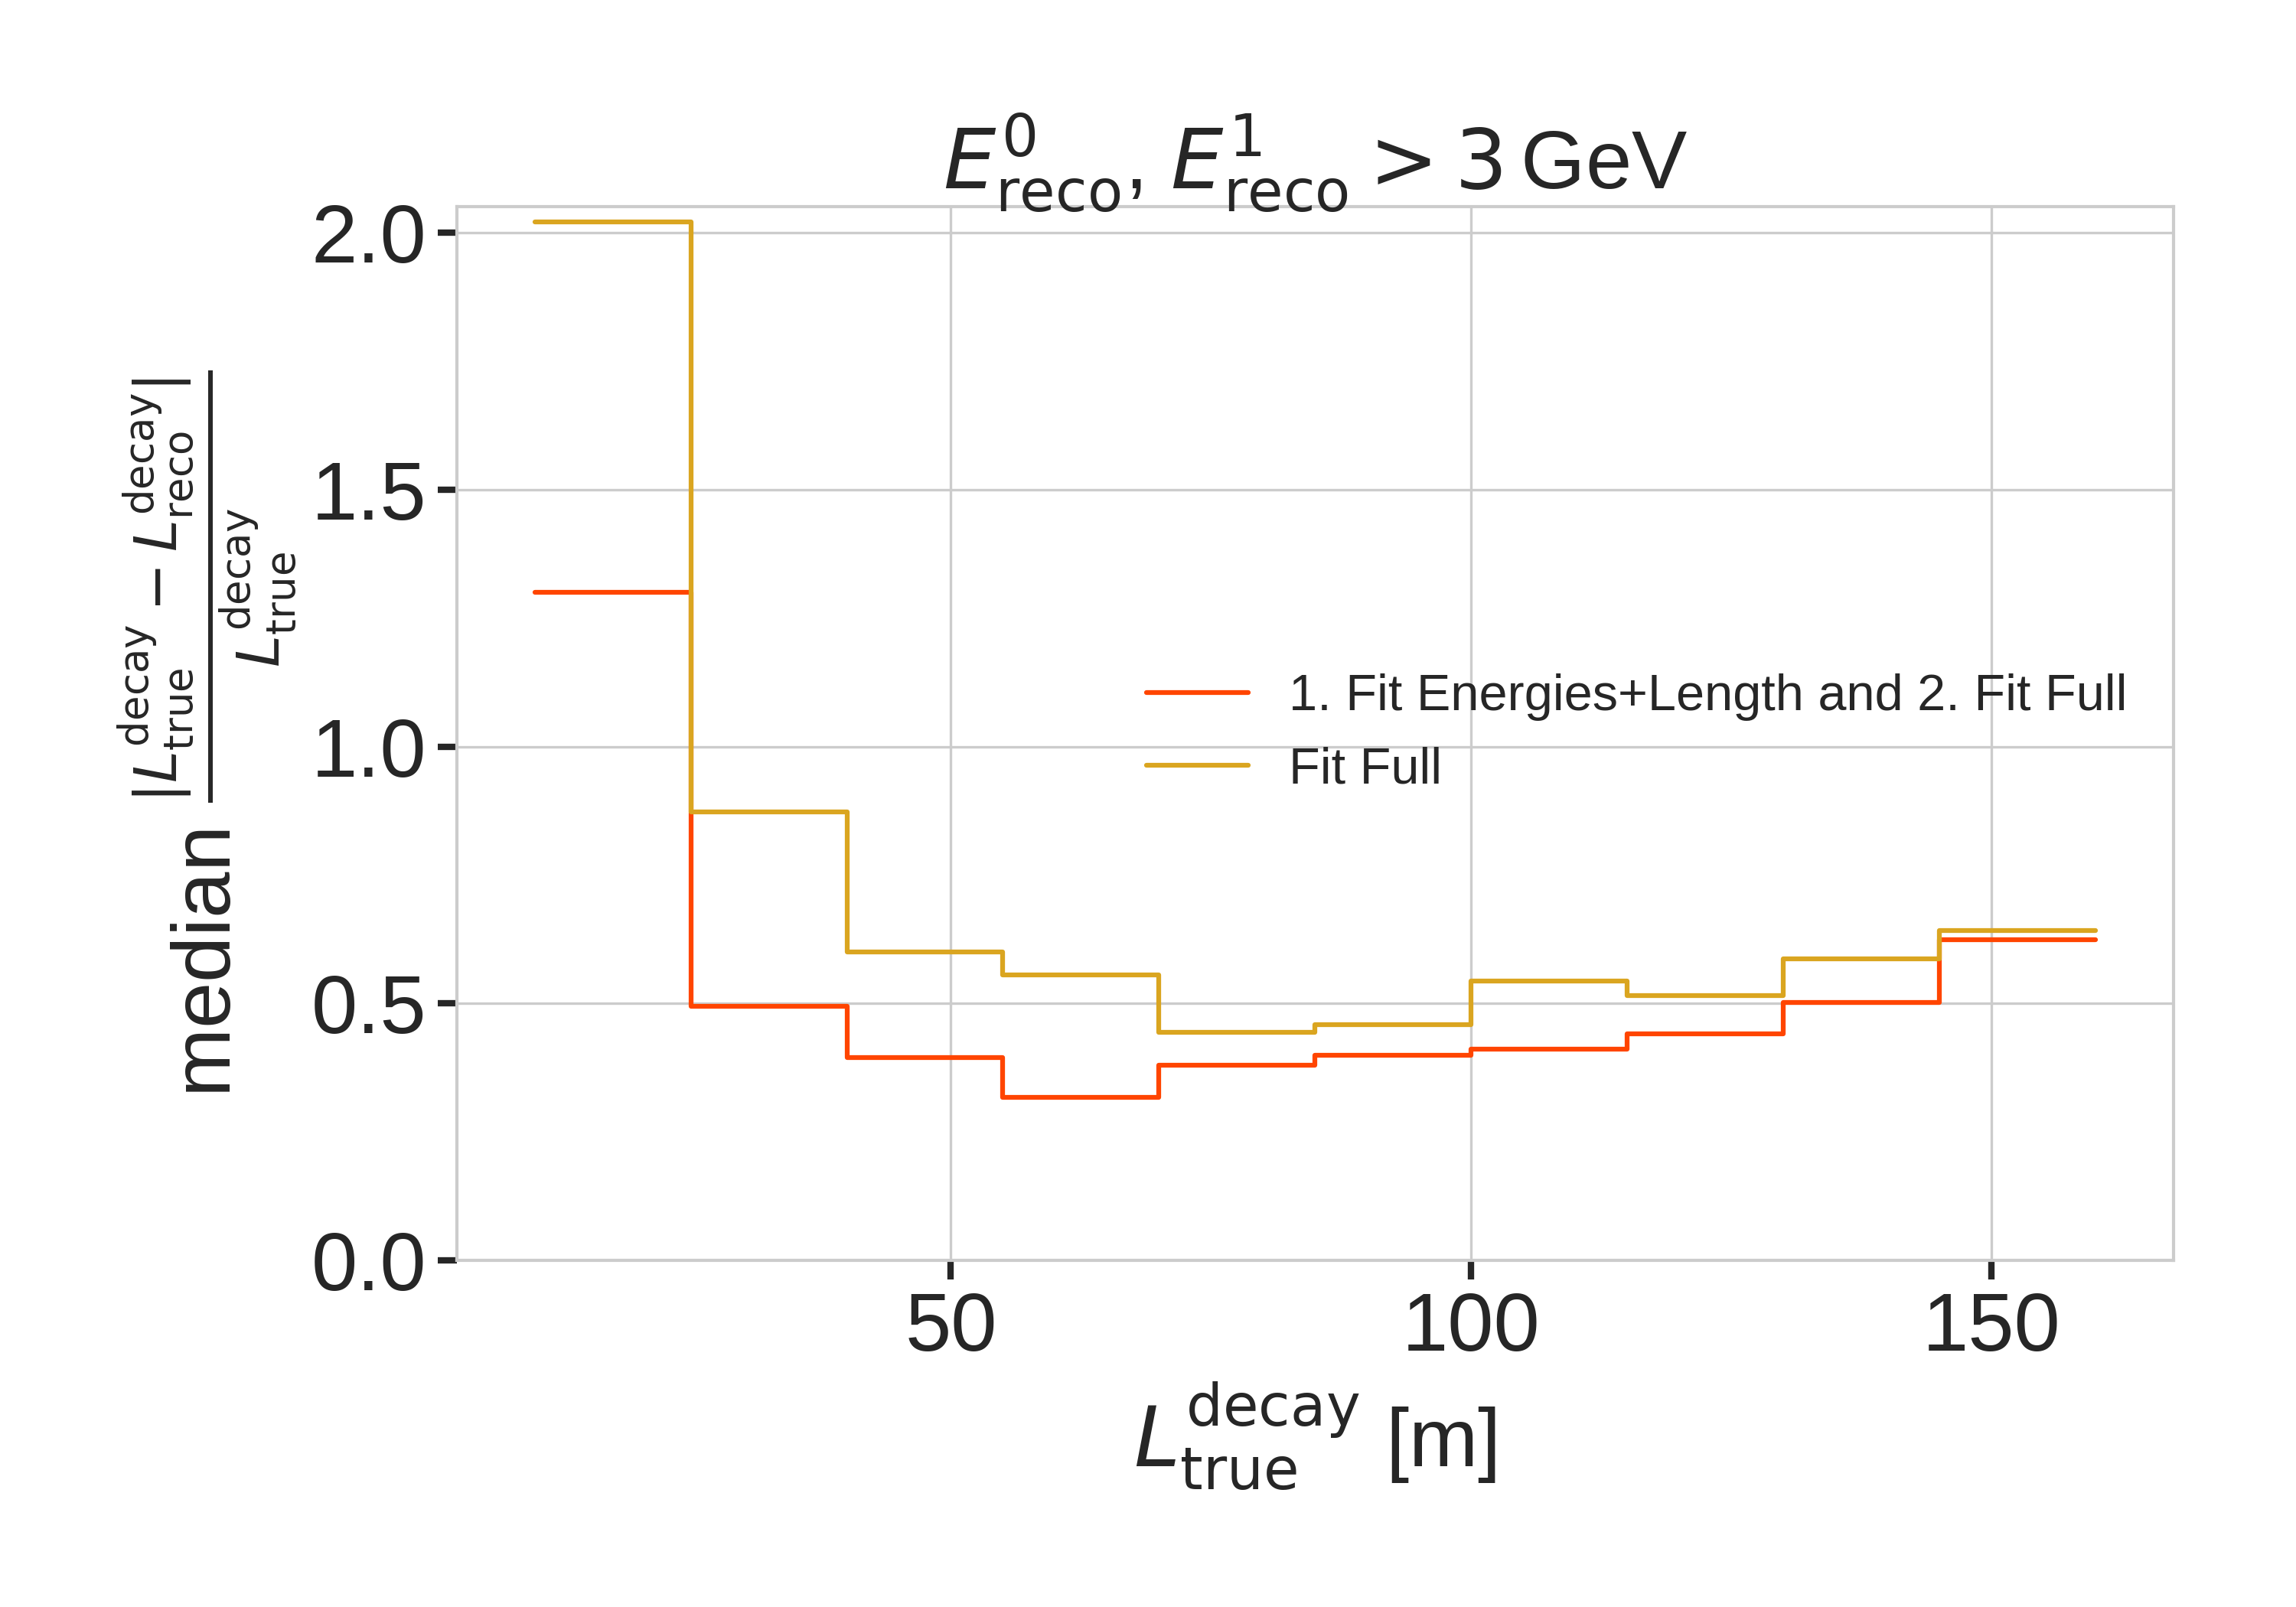
\includegraphics{figures/results/190605_reco_optimization/fit_routine_splitting_median_decay_length_resolution_Good + L7 + reco E1,E2 above 3_fix_y.png}
    \caption[Decay length resolution to optimize fit routine]{Decay length resolution as a function of the true decay length, comparing a full 9 parameters fit to an iterative approach where first the energies and the decay length are fit, while fixing the other 7 parameters and then the full fit is performed. Only events that had more than \SI{3}{\gev} in both cascades are used, and the resolutions are unweighted.}
    \labfig{fit_routine_optimization_fit_routine}
\end{marginfigure}
\todo{Remake with better dimensions, so it fits in the margin, remove or make better title corresponding to the subsubsection titles (RED)}

Because the length seed showed to have such a large impact on the reconstruction performance, a more sophisticated fit routine than fitting all 9 parameters at once was tested. In a first fit iteration, some parameters are fixed and the resulting best fit point is used to fit all 9 parameters in a second iteration. In \reffig{fit_routine_optimization_fit_routine} it can be seen how a fit split into two consecutive steps, where the first step fits only both cascade energies and the decay length and the second step fits the full 9 parameters, performs better as compared to a single, full 9 parameter fit. The initial seed remains identical for both the routines.


\subsubsection{Minimizer Settings}

\begin{marginfigure}
	\centering
    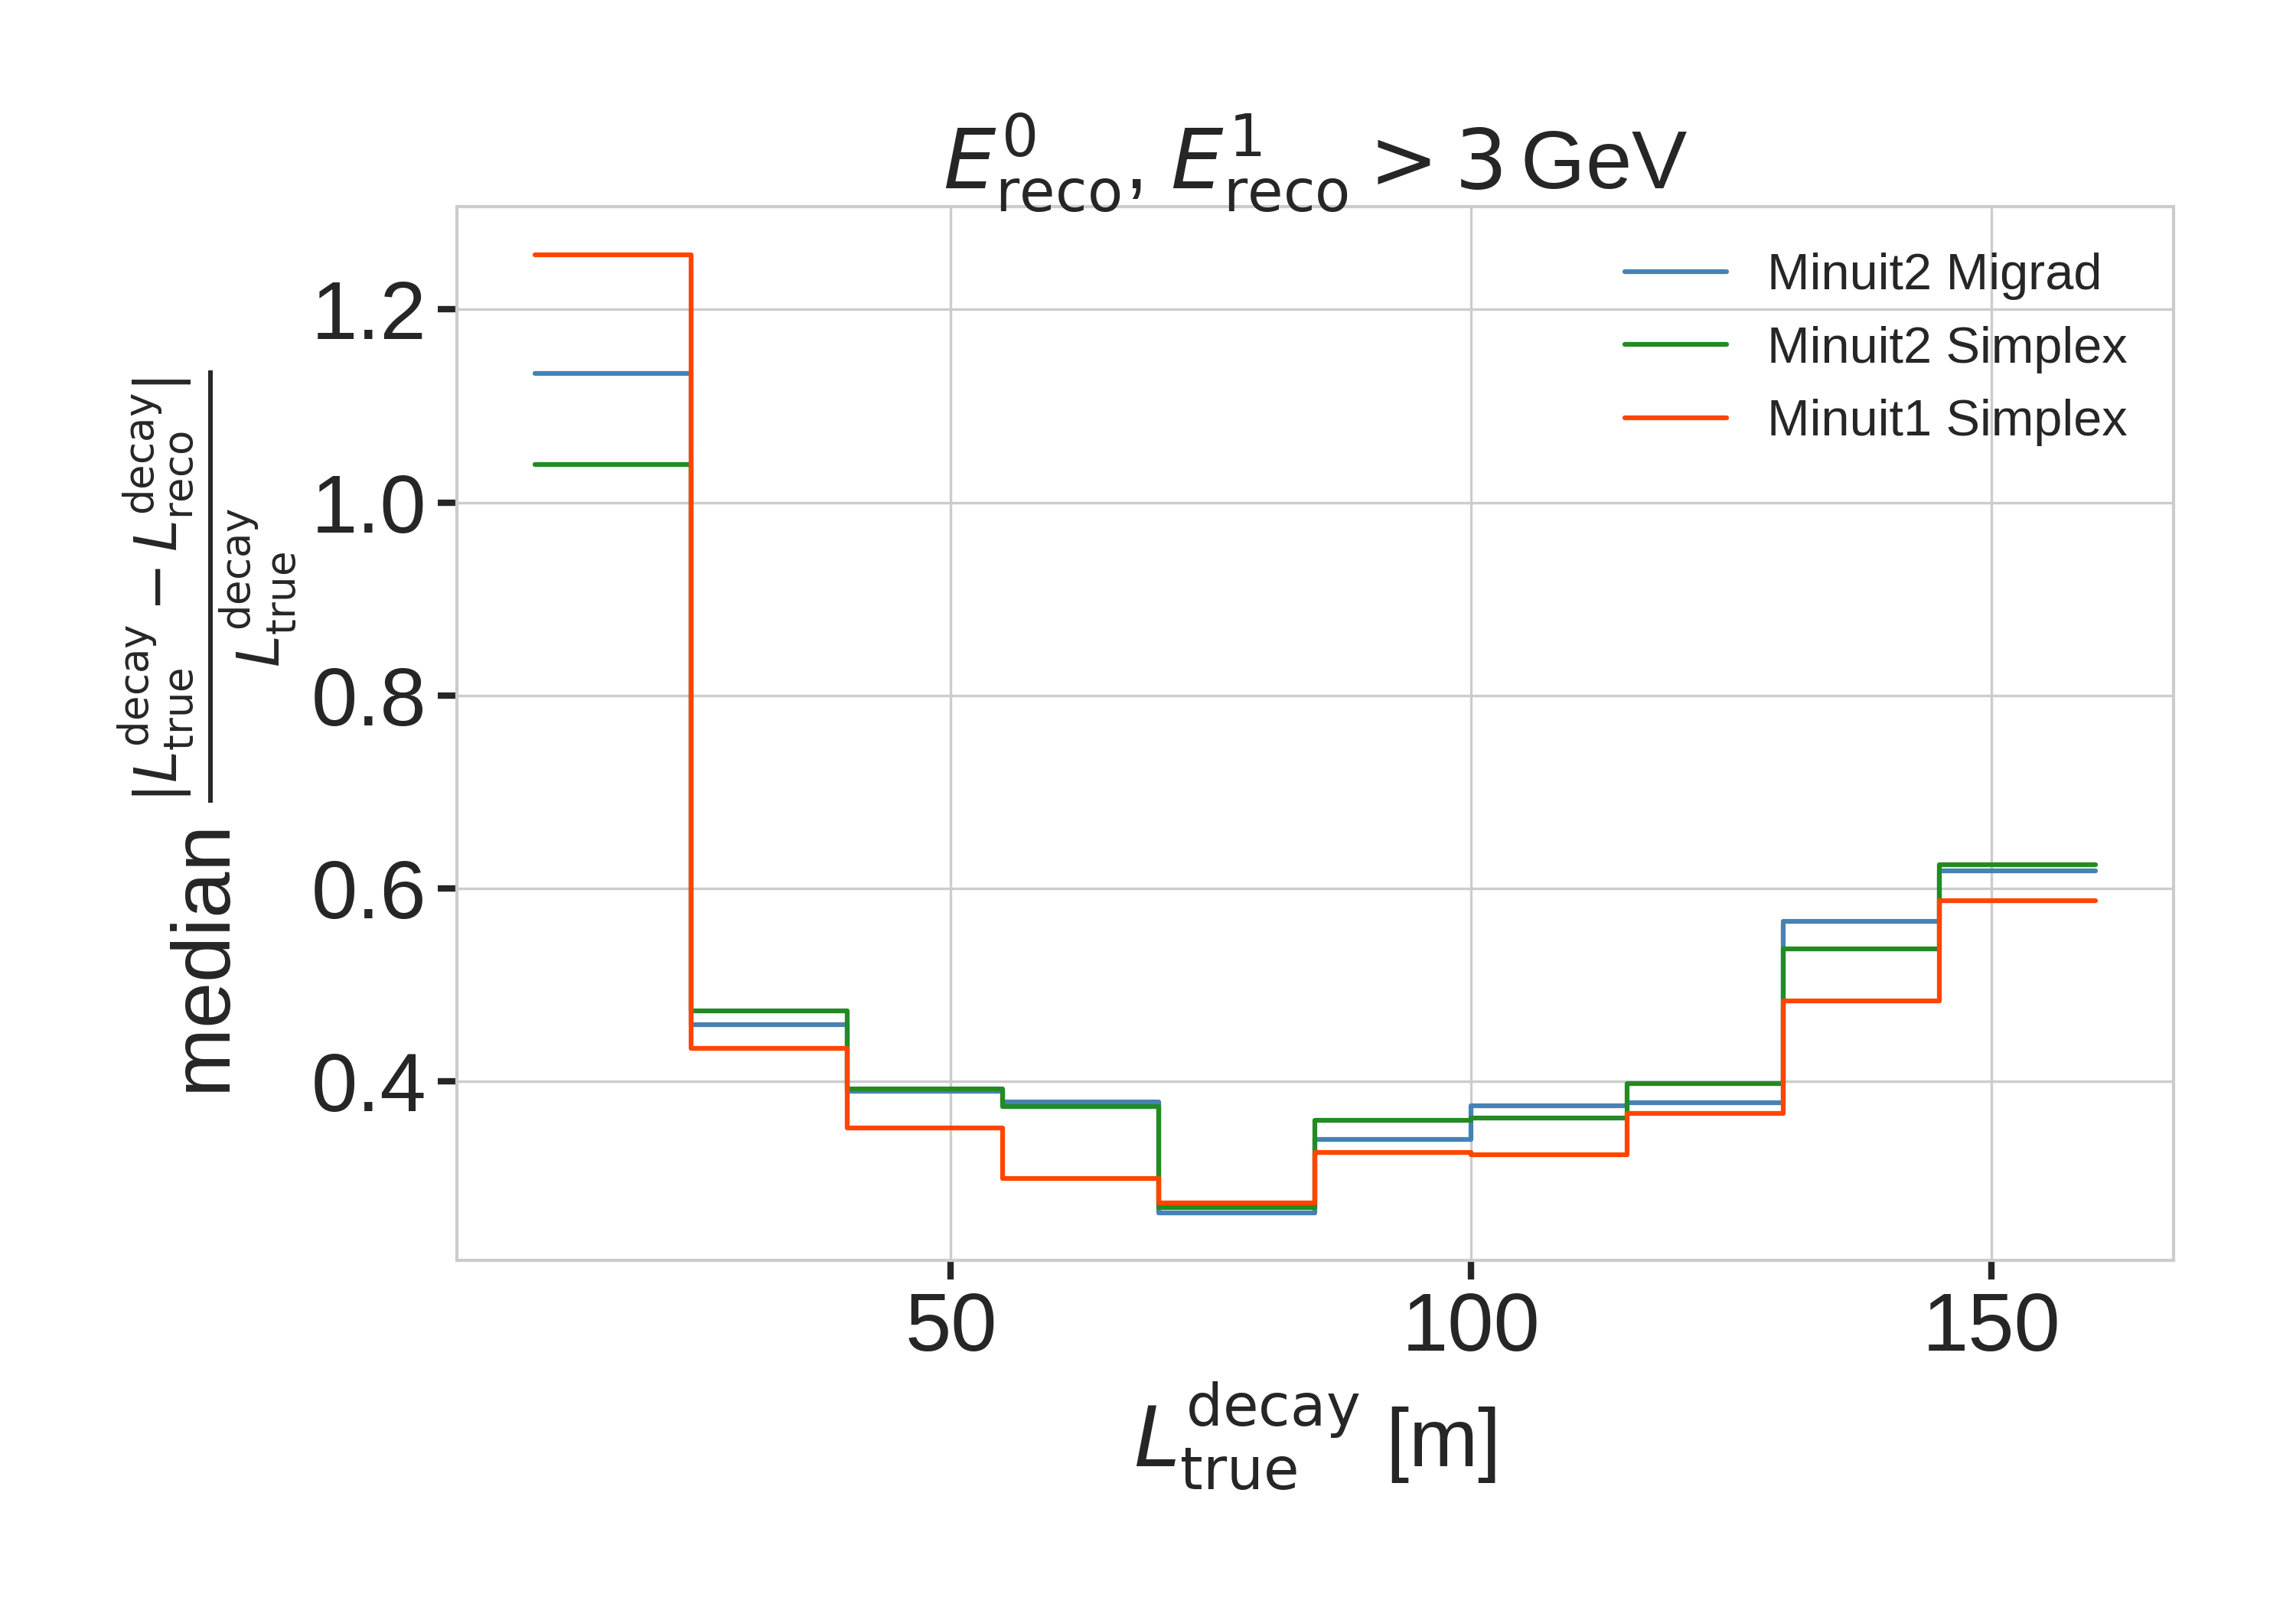
\includegraphics{figures/results/190605_reco_optimization/minimizer_checks_median_decay_length_resolution_Good + L7 + reco E1,E2 above 3.png}
    \caption[Decay length resolution to optimize minimizer settings]{Decay length resolution as a function of the true decay length, comparing the same fit routine performed with different minimizers. Only events that had more than \SI{3}{\gev} in both cascades are used, and the resolutions are unweighted.}
    \labfig{fit_routine_optimization_minimizer_checks}
\end{marginfigure}
\todo{Remake with better dimensions, so it fits in the margin, remove or make better title corresponding to the subsubsection titles (RED)}

To investigate the effect of the minimizer used to find the best fit parameters, the reconstruction was performed using three different minimizers, which were easily accessible within the reconstruction framework. The minimizers used were Minuit1 Simplex, Minuit2 Simplex, and Minuit2 Migrad\todo{cite these buggers again, and or point back to where they were mentioned? (RED)}. The initial idea was to test a global minimizer, or a routine that can find the rough position of the global minimum first and then a local minimizer to find the exact minimum, but unfortunately this was not possible with the minimizers available in the framework. As can be seen in \reffig{fit_routine_optimization_minimizer_checks}, Minuit1 Simplex performed best and was chosen as the default for the reconstruction.


% \begin{figure*}[h]
% 	\centering
%     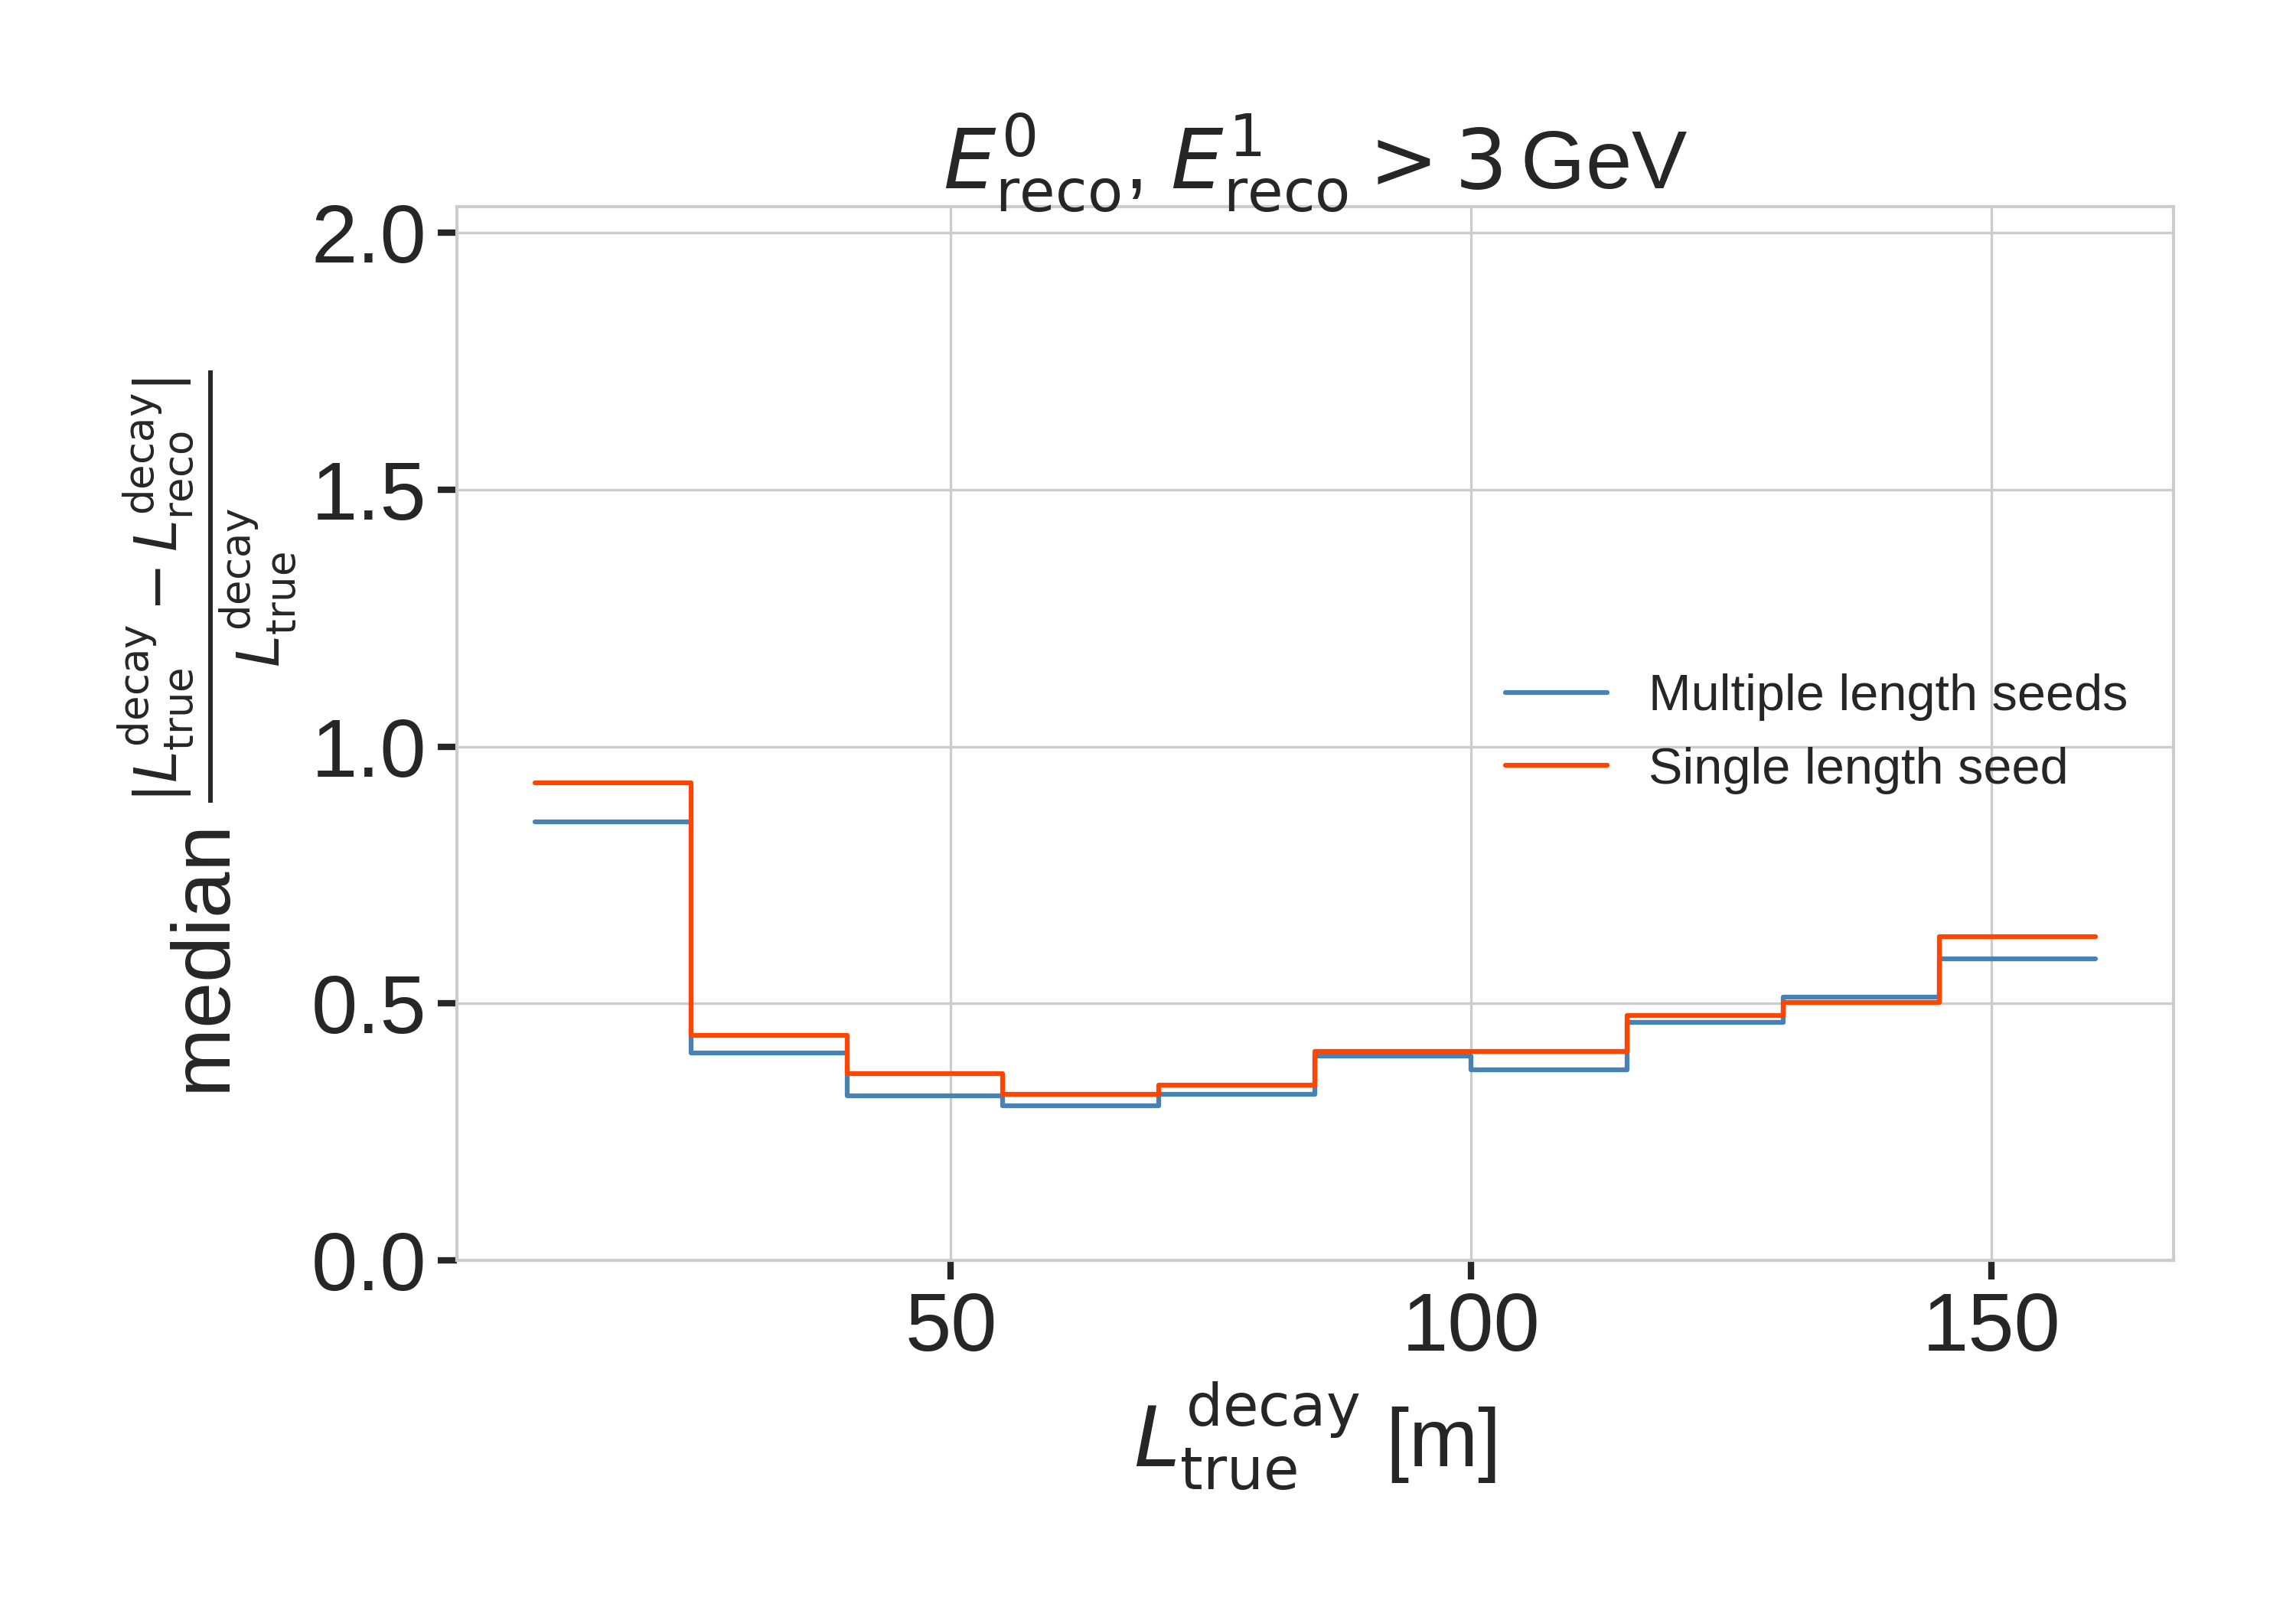
\includegraphics[width=0.32\linewidth]{figures/results/190605_reco_optimization/decay_length_seeding_median_decay_length_resolution_Good + L7 + reco E1,E2 above 3_fix_y.png}
%     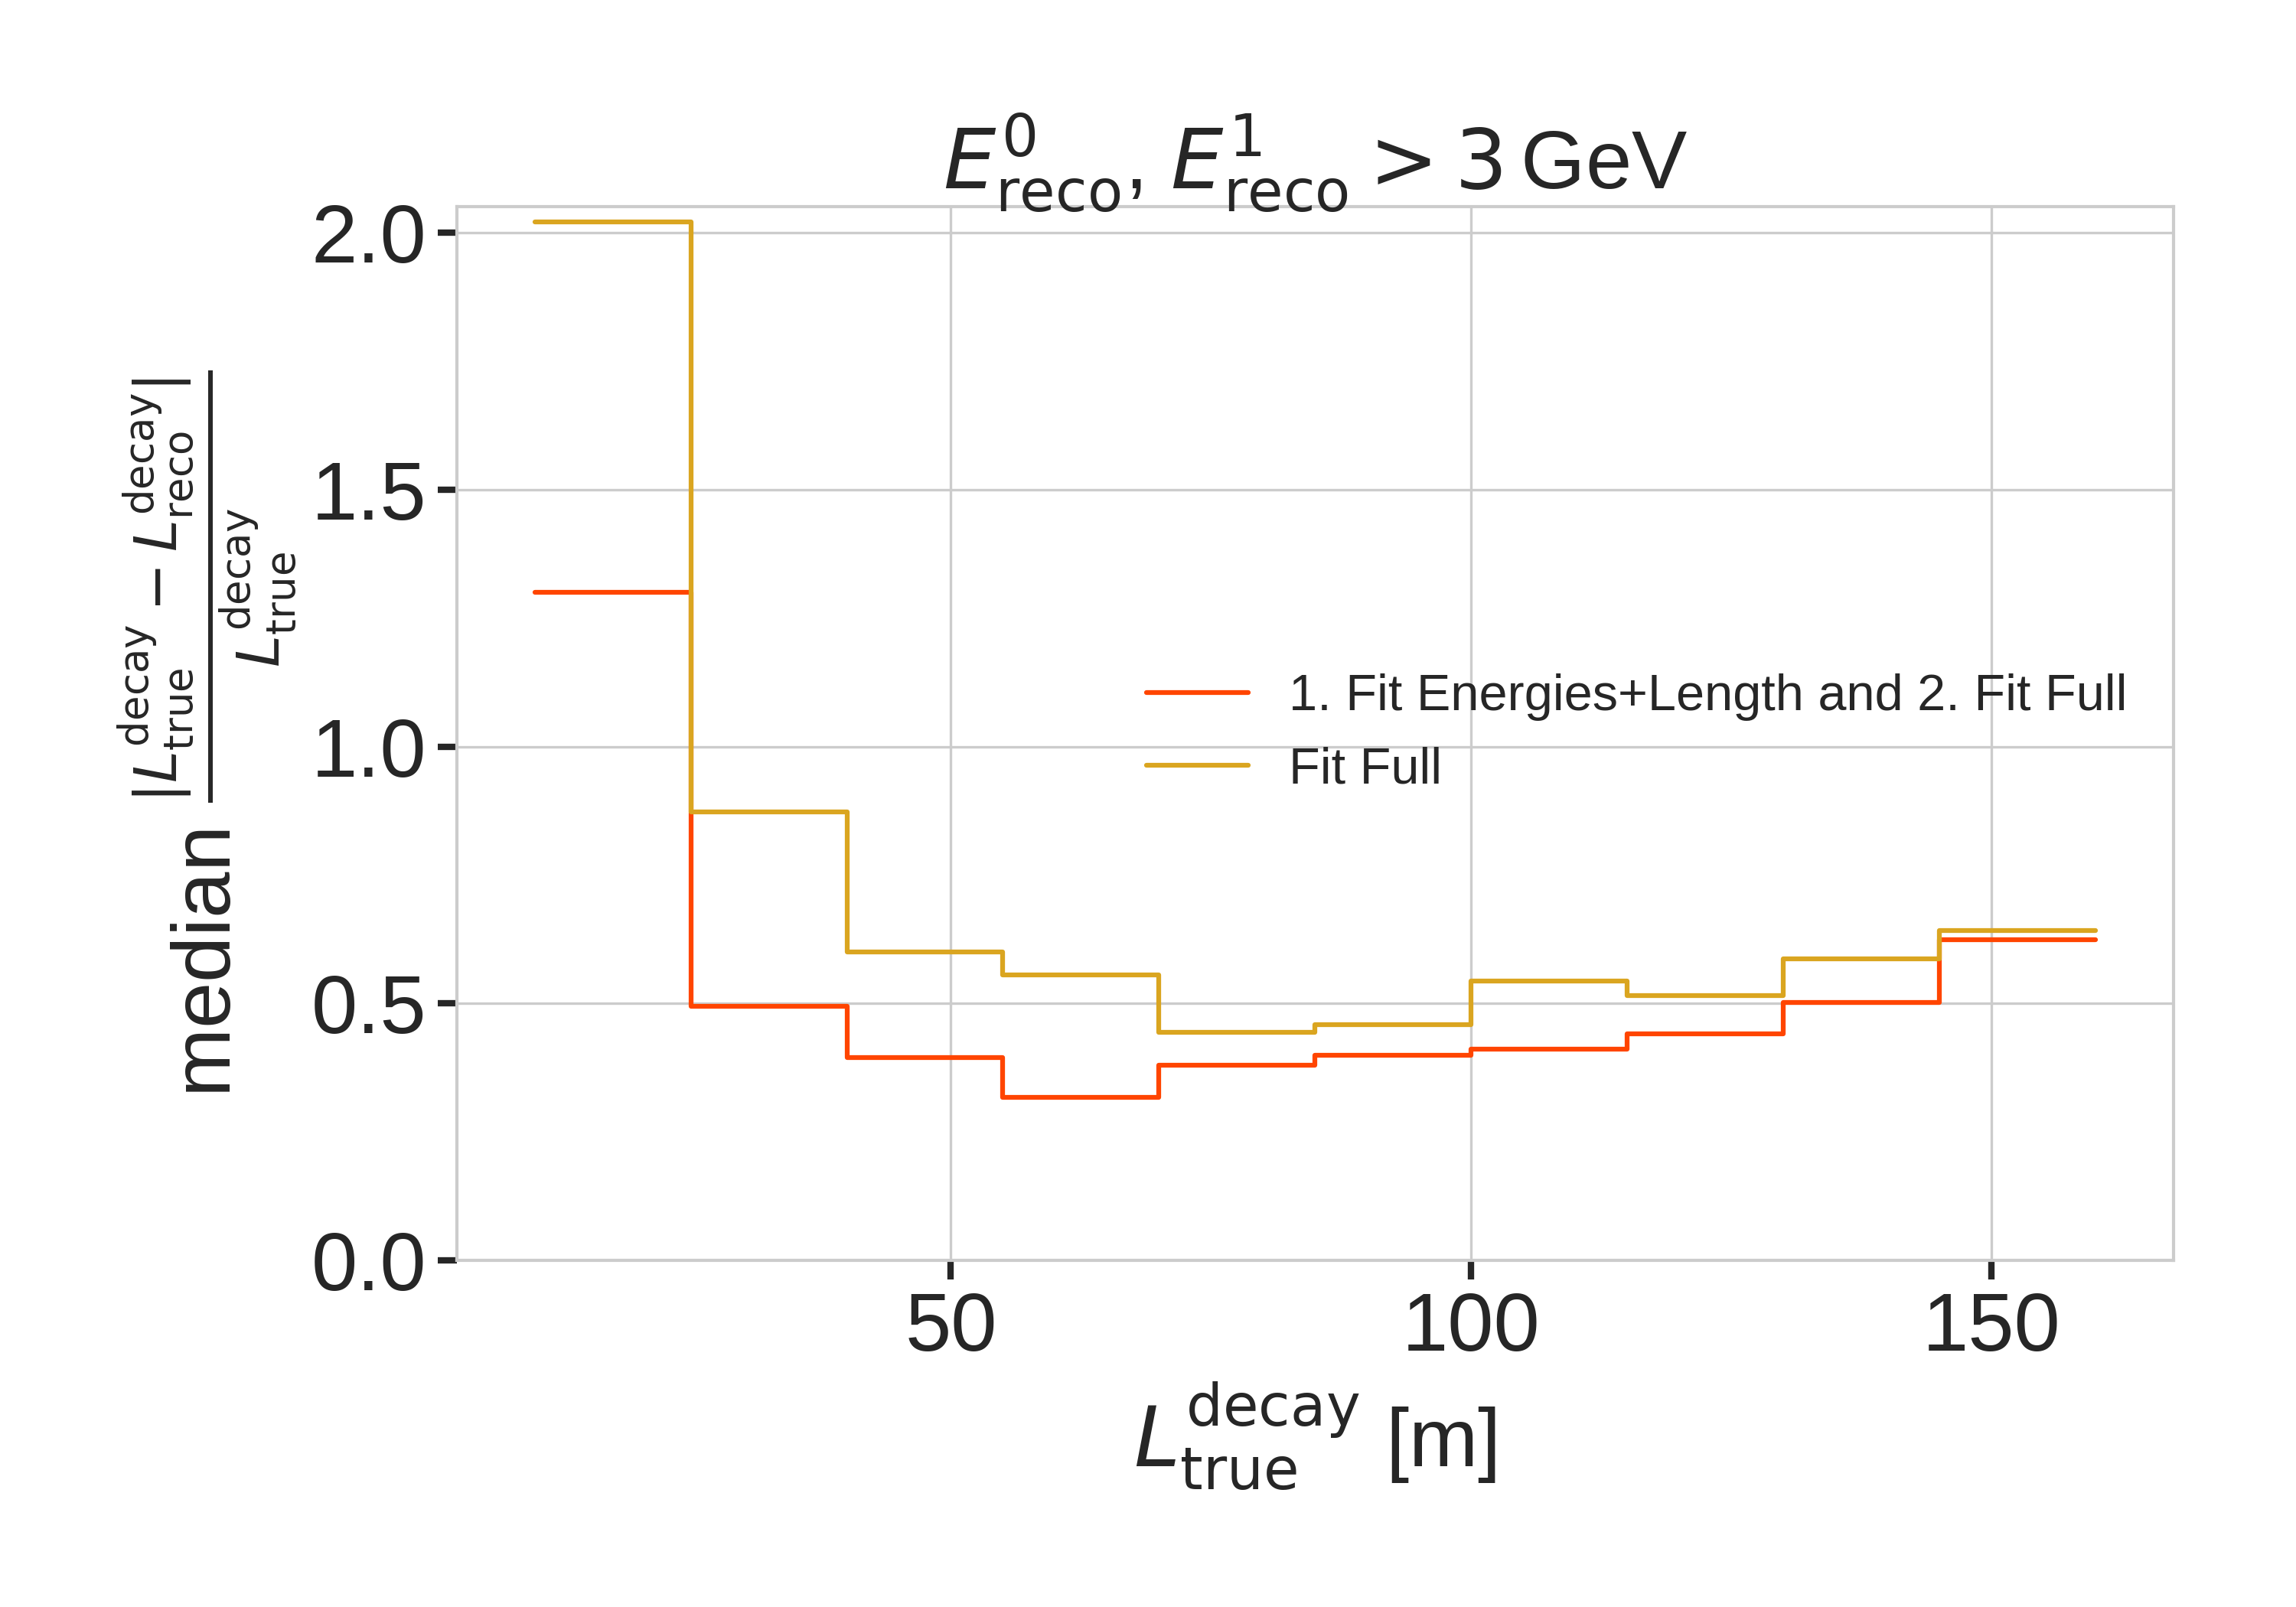
\includegraphics[width=0.32\linewidth]{figures/results/190605_reco_optimization/fit_routine_splitting_median_decay_length_resolution_Good + L7 + reco E1,E2 above 3_fix_y.png}
%     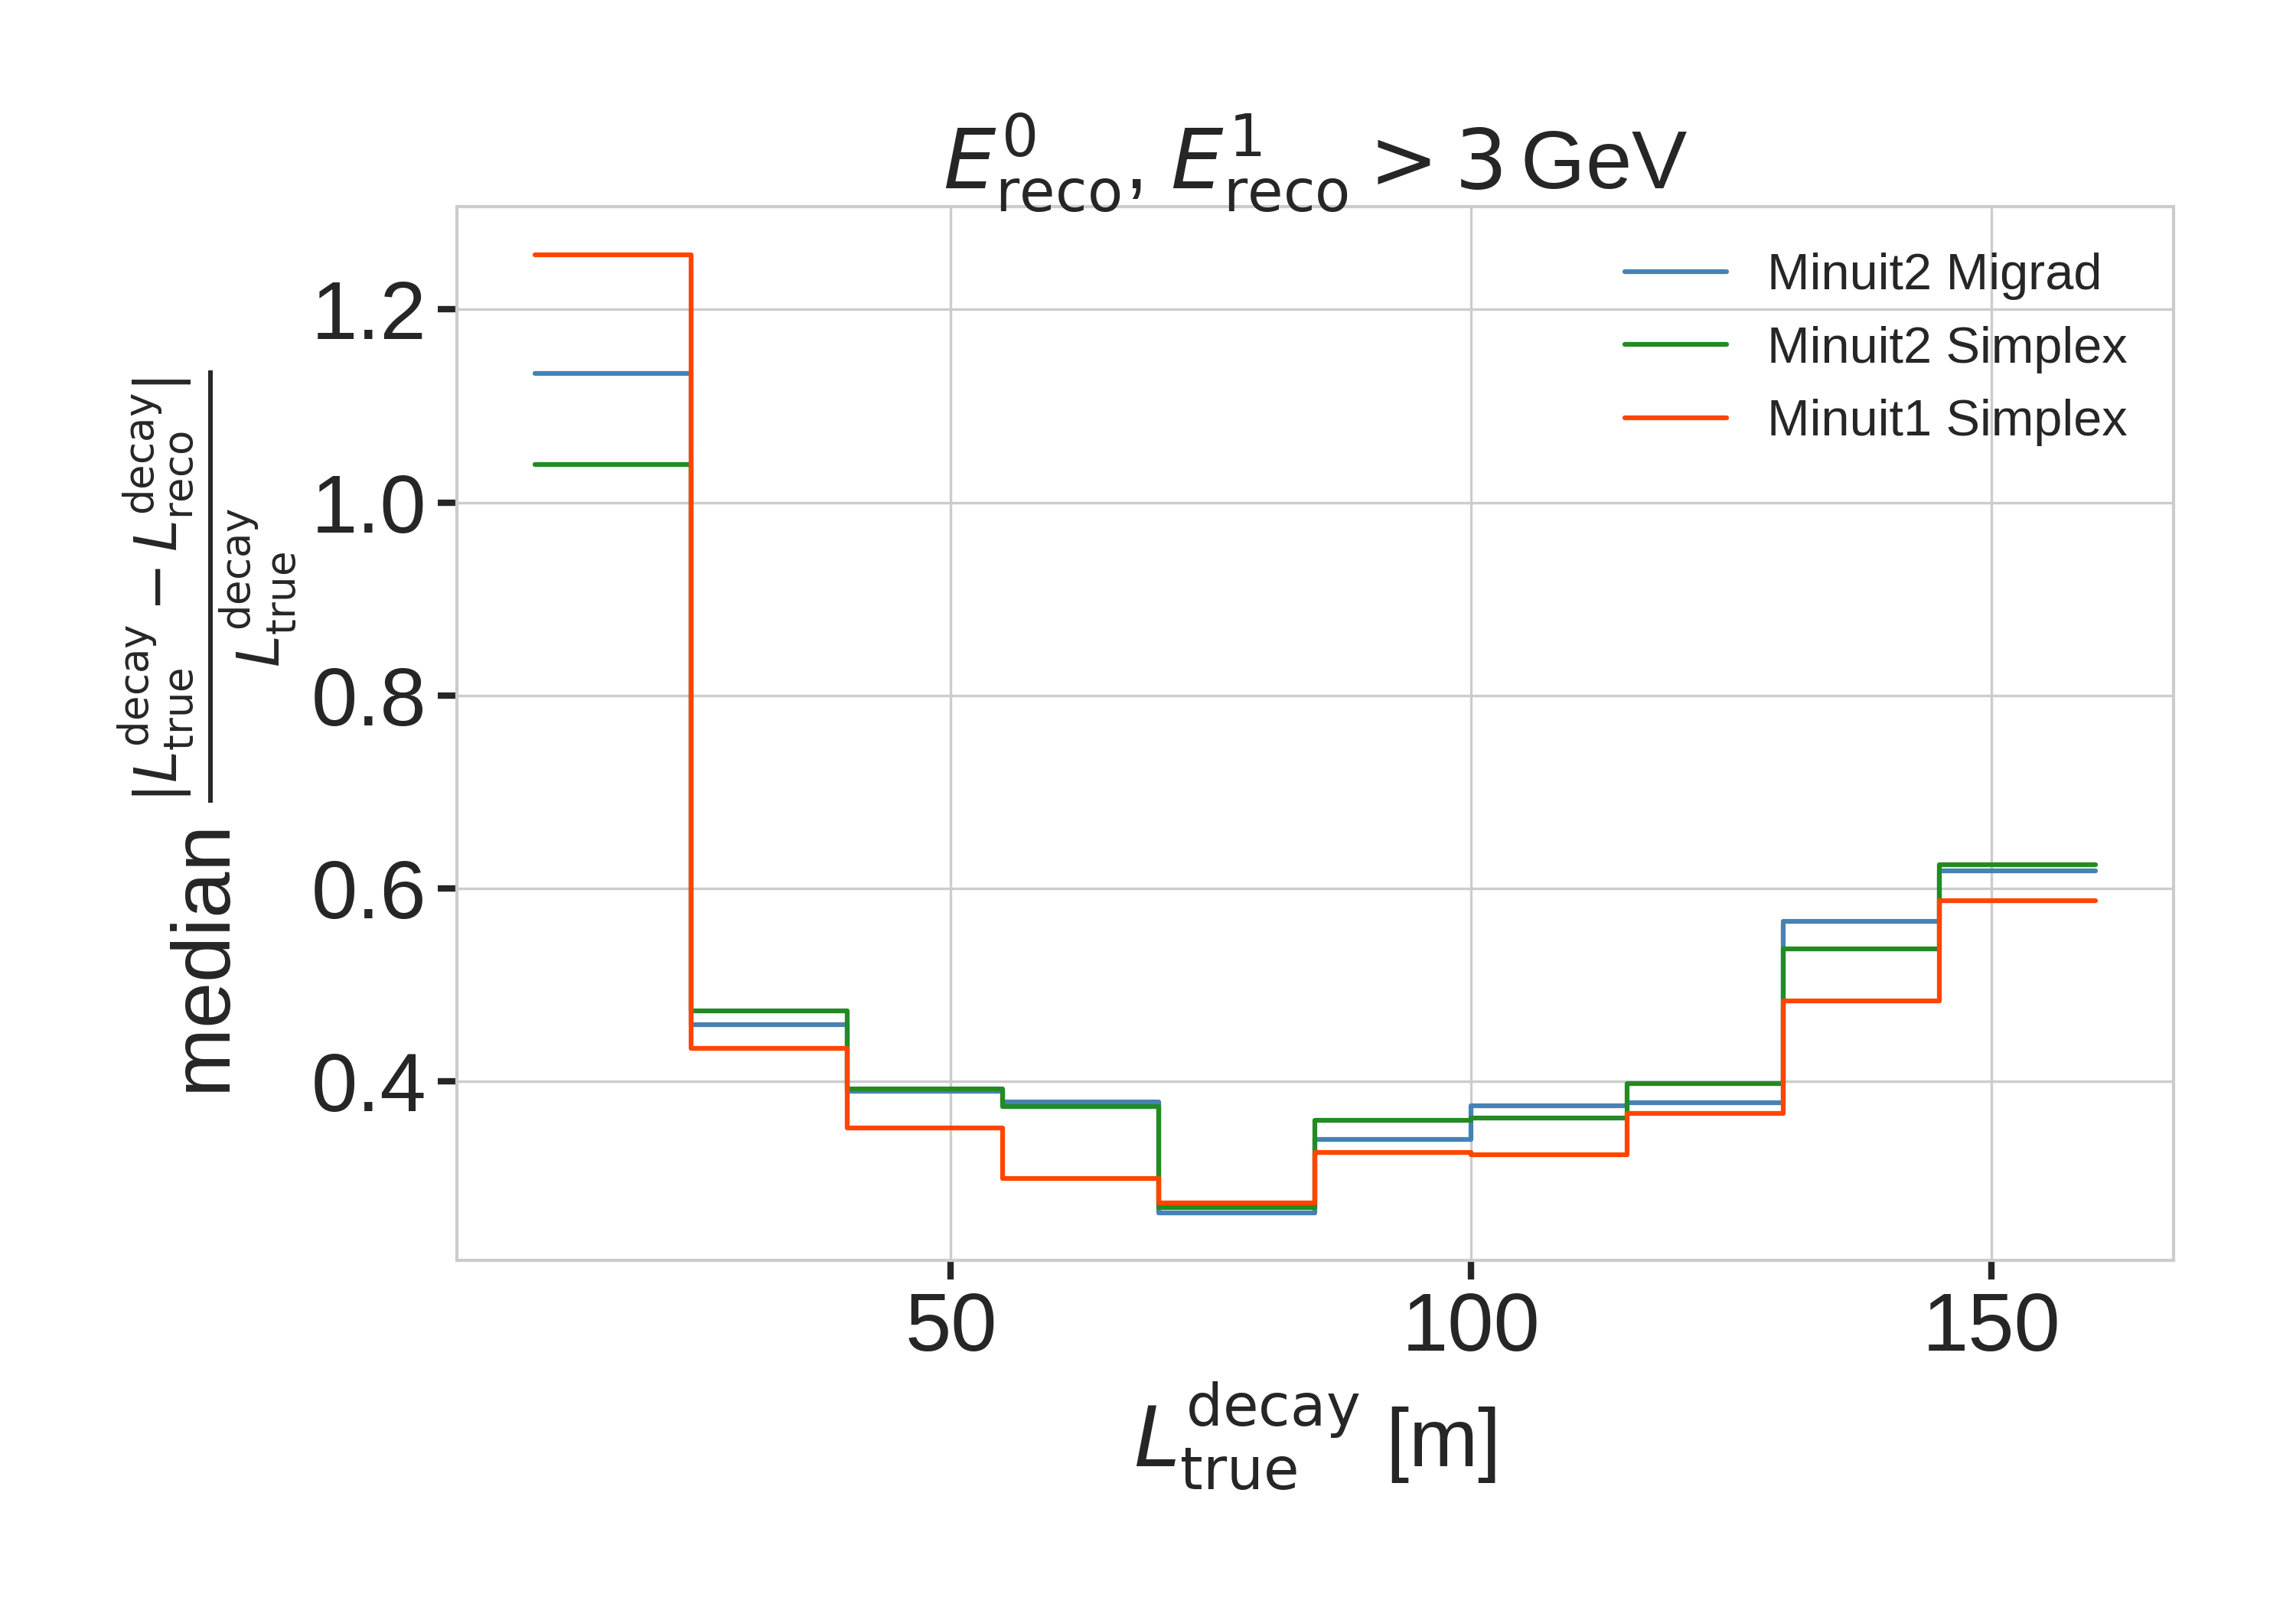
\includegraphics[width=0.32\linewidth]{figures/results/190605_reco_optimization/minimizer_checks_median_decay_length_resolution_Good + L7 + reco E1,E2 above 3.png}
%     \caption[]{Decay length resolution as a function of the true decay length, comparing the same fit routine seeded with just the seed decay length and seeded with a decay length of \SI{5}{\meter}, \SI{25}{\meter}, \SI{50}{\meter}, \SI{100}{\meter}, and \SI{200}{\meter} on the left. The middle panel compares a full 9 parameters fit to an iterative approach where first the energies and the decay length are fit, while fixing the other 7 parameters and then the full fit is performed. The right panel compares the same fit routine performed with different minimizers. The resolutions are unweighted.}
%     \labfig{fit_routine_optimization}
% \end{figure*}
% \todo{Remake them with better dimensions, so it's visible side by side, remove or make better title? Corresponding to the subsubsection titles (RED)}


\subsection{Performance}

The chosen reconstruction chain used to test the performance of the detector to observe low energy double cascades is the following; Minuit1 Simplex is used as the minimizer, the decay length is seeded with 3 different values, 0.5x, 1.0x, and 1.5x the length of the preceding track reconstruction, and the fit routine is split into two steps, where the first step fits the energies and the decay length and the second step fits the full 9 parameters. In the first step, the number of time bins in \refeq{millipede_likelihood} is set to 1, so just the number of photons and their spatial information is used. The second step is seeded with the best results from the first step, and here the number of time bins is chosen such that each photon falls into a separate time bin, which means all time information is used. The average runtime per event is $\sim$\SI{16}{\second} on a single CPU core, but is very dependent on the number of photons observed in the event, since the likelihood calculation in the second step scales with this number and a table lookup has to be performed for each photon.

To get a more realistic estimate of the reconstruction performance, it is run on a second preliminary sample of HNL events from the model dependent simulation, containing masses between \SIrange[range-phrase=~and~]{0.1}{3.0}{\gev} and the lab frame decay length is sampled from an inverse distribution in the range from \SIrange{1}{1000}{\meter}, which is a better approximation of the expected exponential decay distribution of the HNL. The performance is shown for events where the reconstruction chain was successfully run, the event selection criteria up to the final selection level of low energy analyses are fulfilled, and the reconstructed energy of both cascades is above \SI{3}{\gev}.


\subsubsection{Energy Resolutions} \labsec{190607_energy_resolutions}

The energy resolution is inspected by looking at the two-dimensional distribution of reconstructed energy versus the true energy as shown in \reffig{selected_routine_2d_energy_results}. The bin entries are shown as well as the median and $\pm$\SI{25}{\percent} calculated per vertical column, to get an idea of the distribution for a given energy slice. The color scale is showing the PDF along each true energy slice, which is the full information highlighted by the median $\pm$\SI{25}{\percent} quantile lines. The reconstructed energy is only the energy that is observable from photons, while the true energy is the total cascade energy, including the parts that go into EM neutral particles that do not produce light. It is therefore expected that the reconstructed energy is lower than the true and the median therefore does not line up with the axis diagonal.

\begin{figure*}[h]
	\centering
    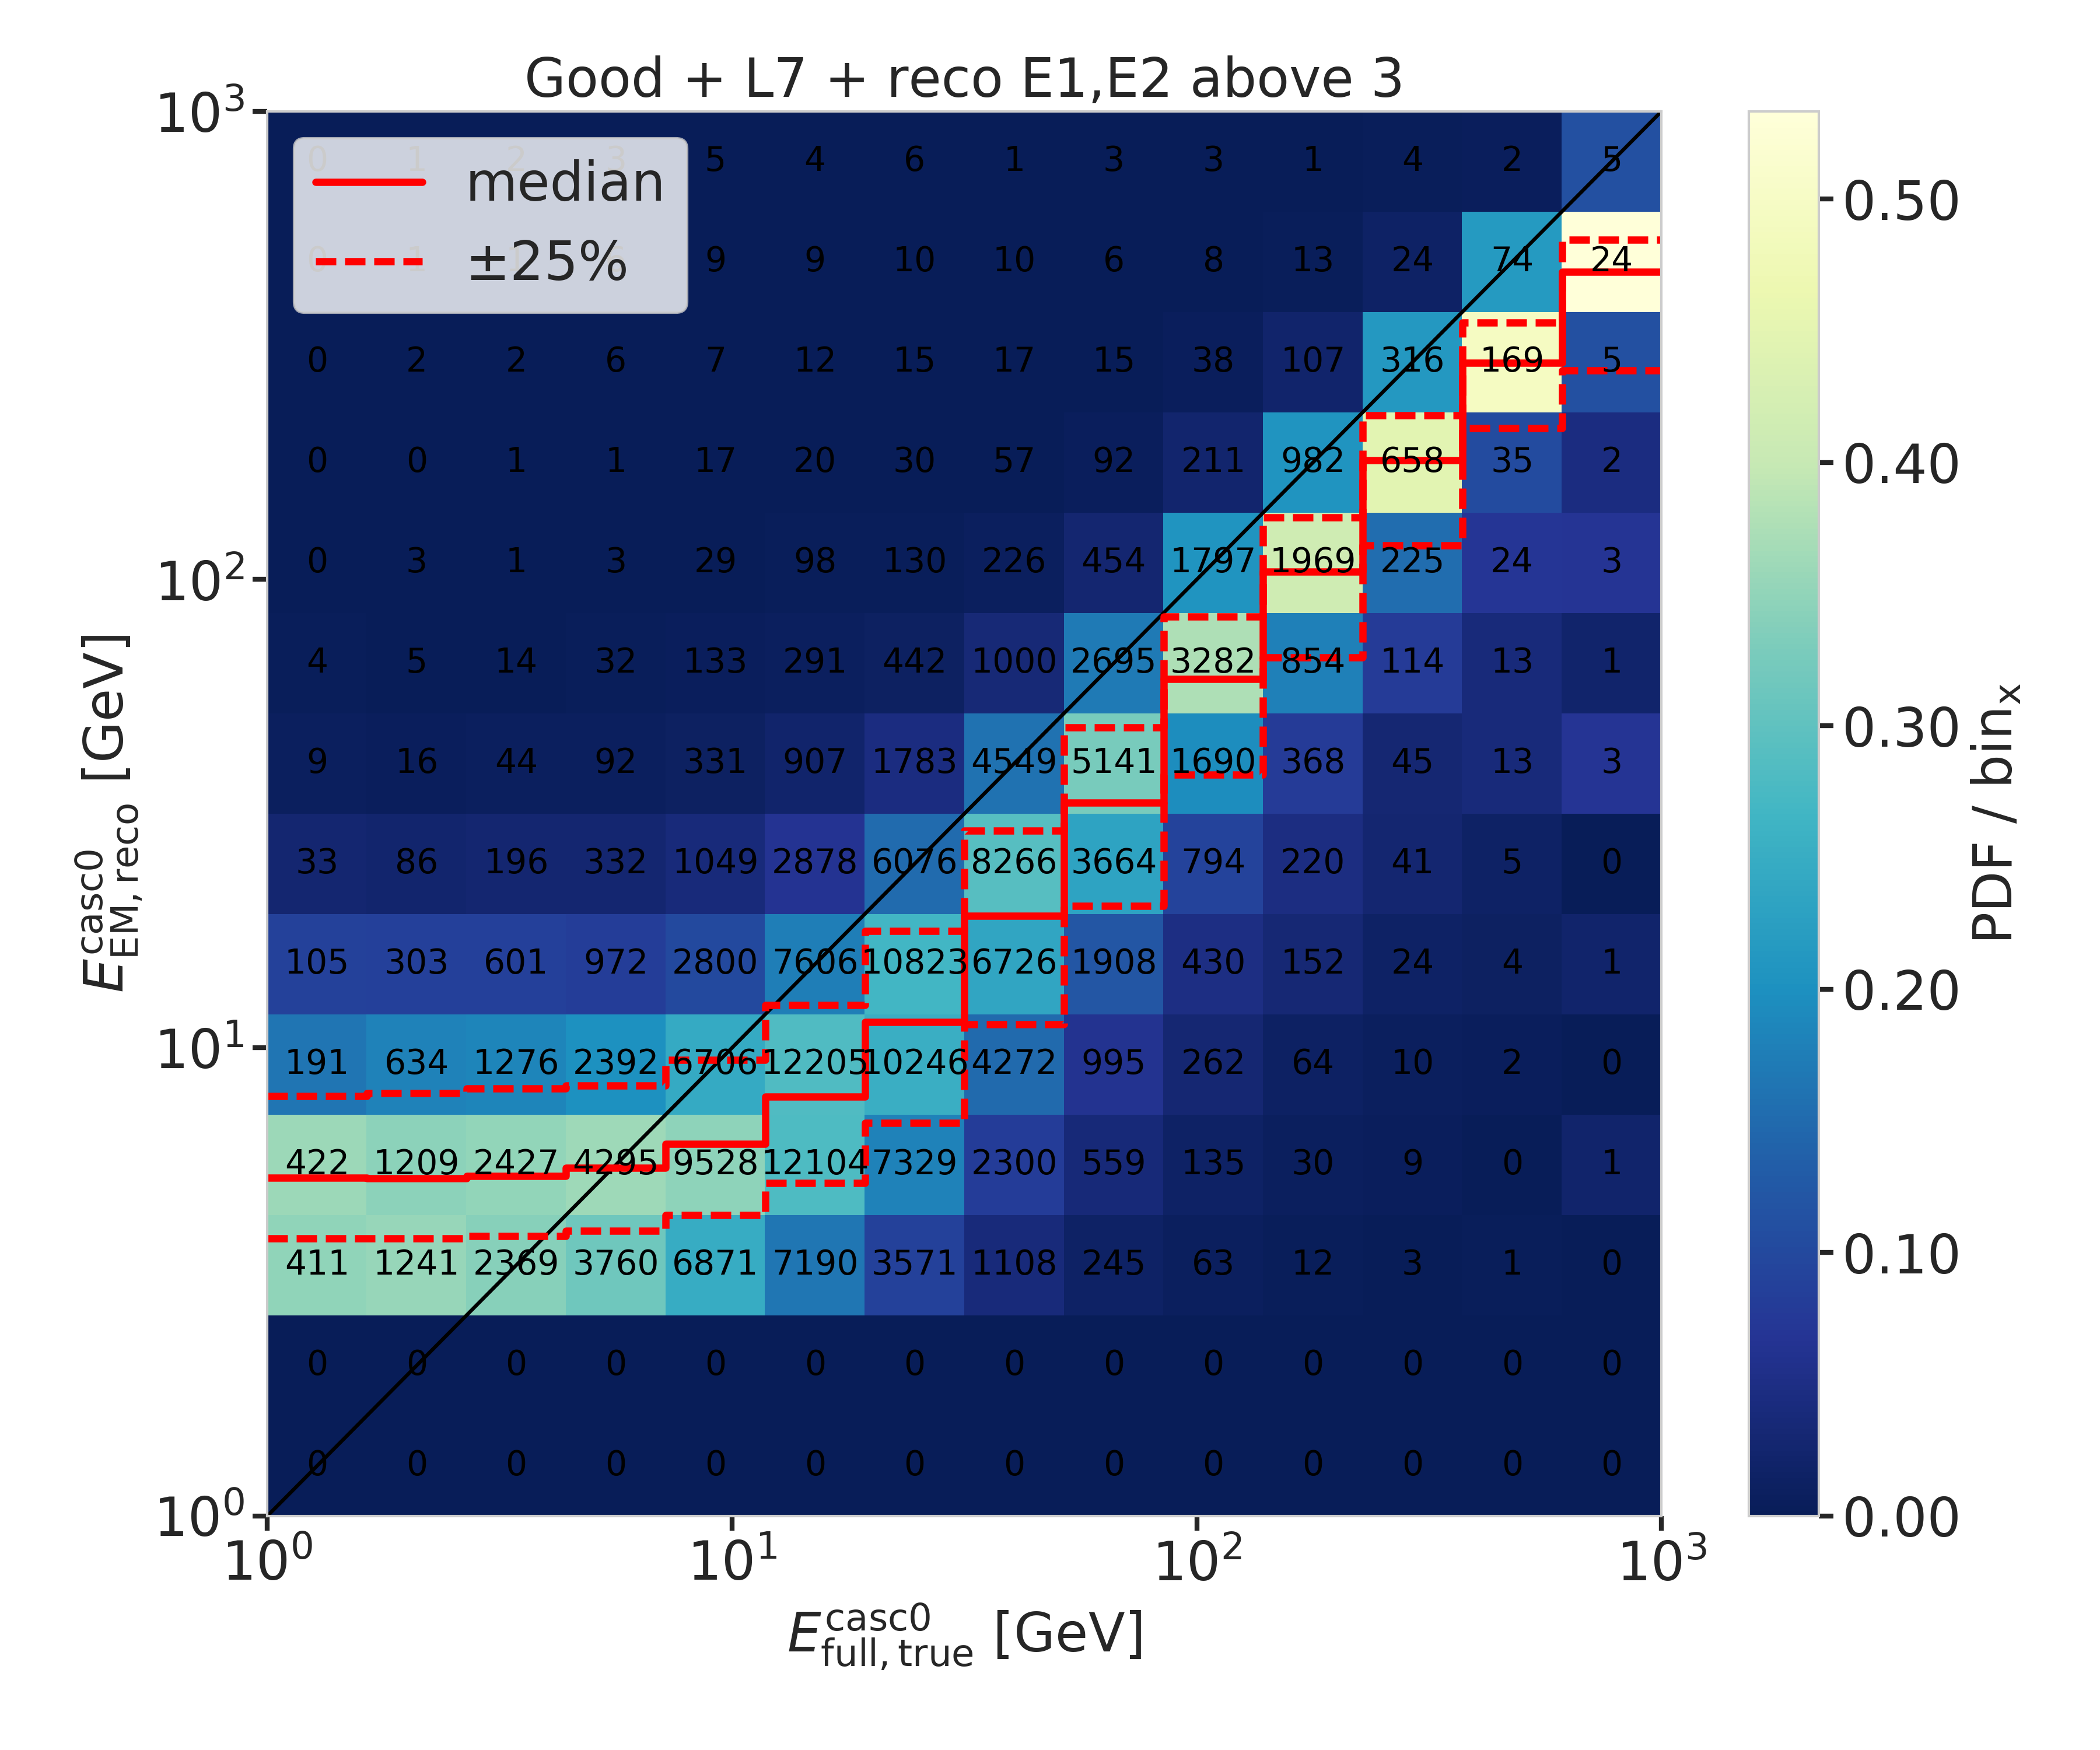
\includegraphics[width=0.49\linewidth]{figures/results/190607/resolutions/190607_millipede_level_no_NaNs_NEW_flipped_casc0_reco_energy_vs_casc0_true_energy_reco_above3_step_contours.png}
    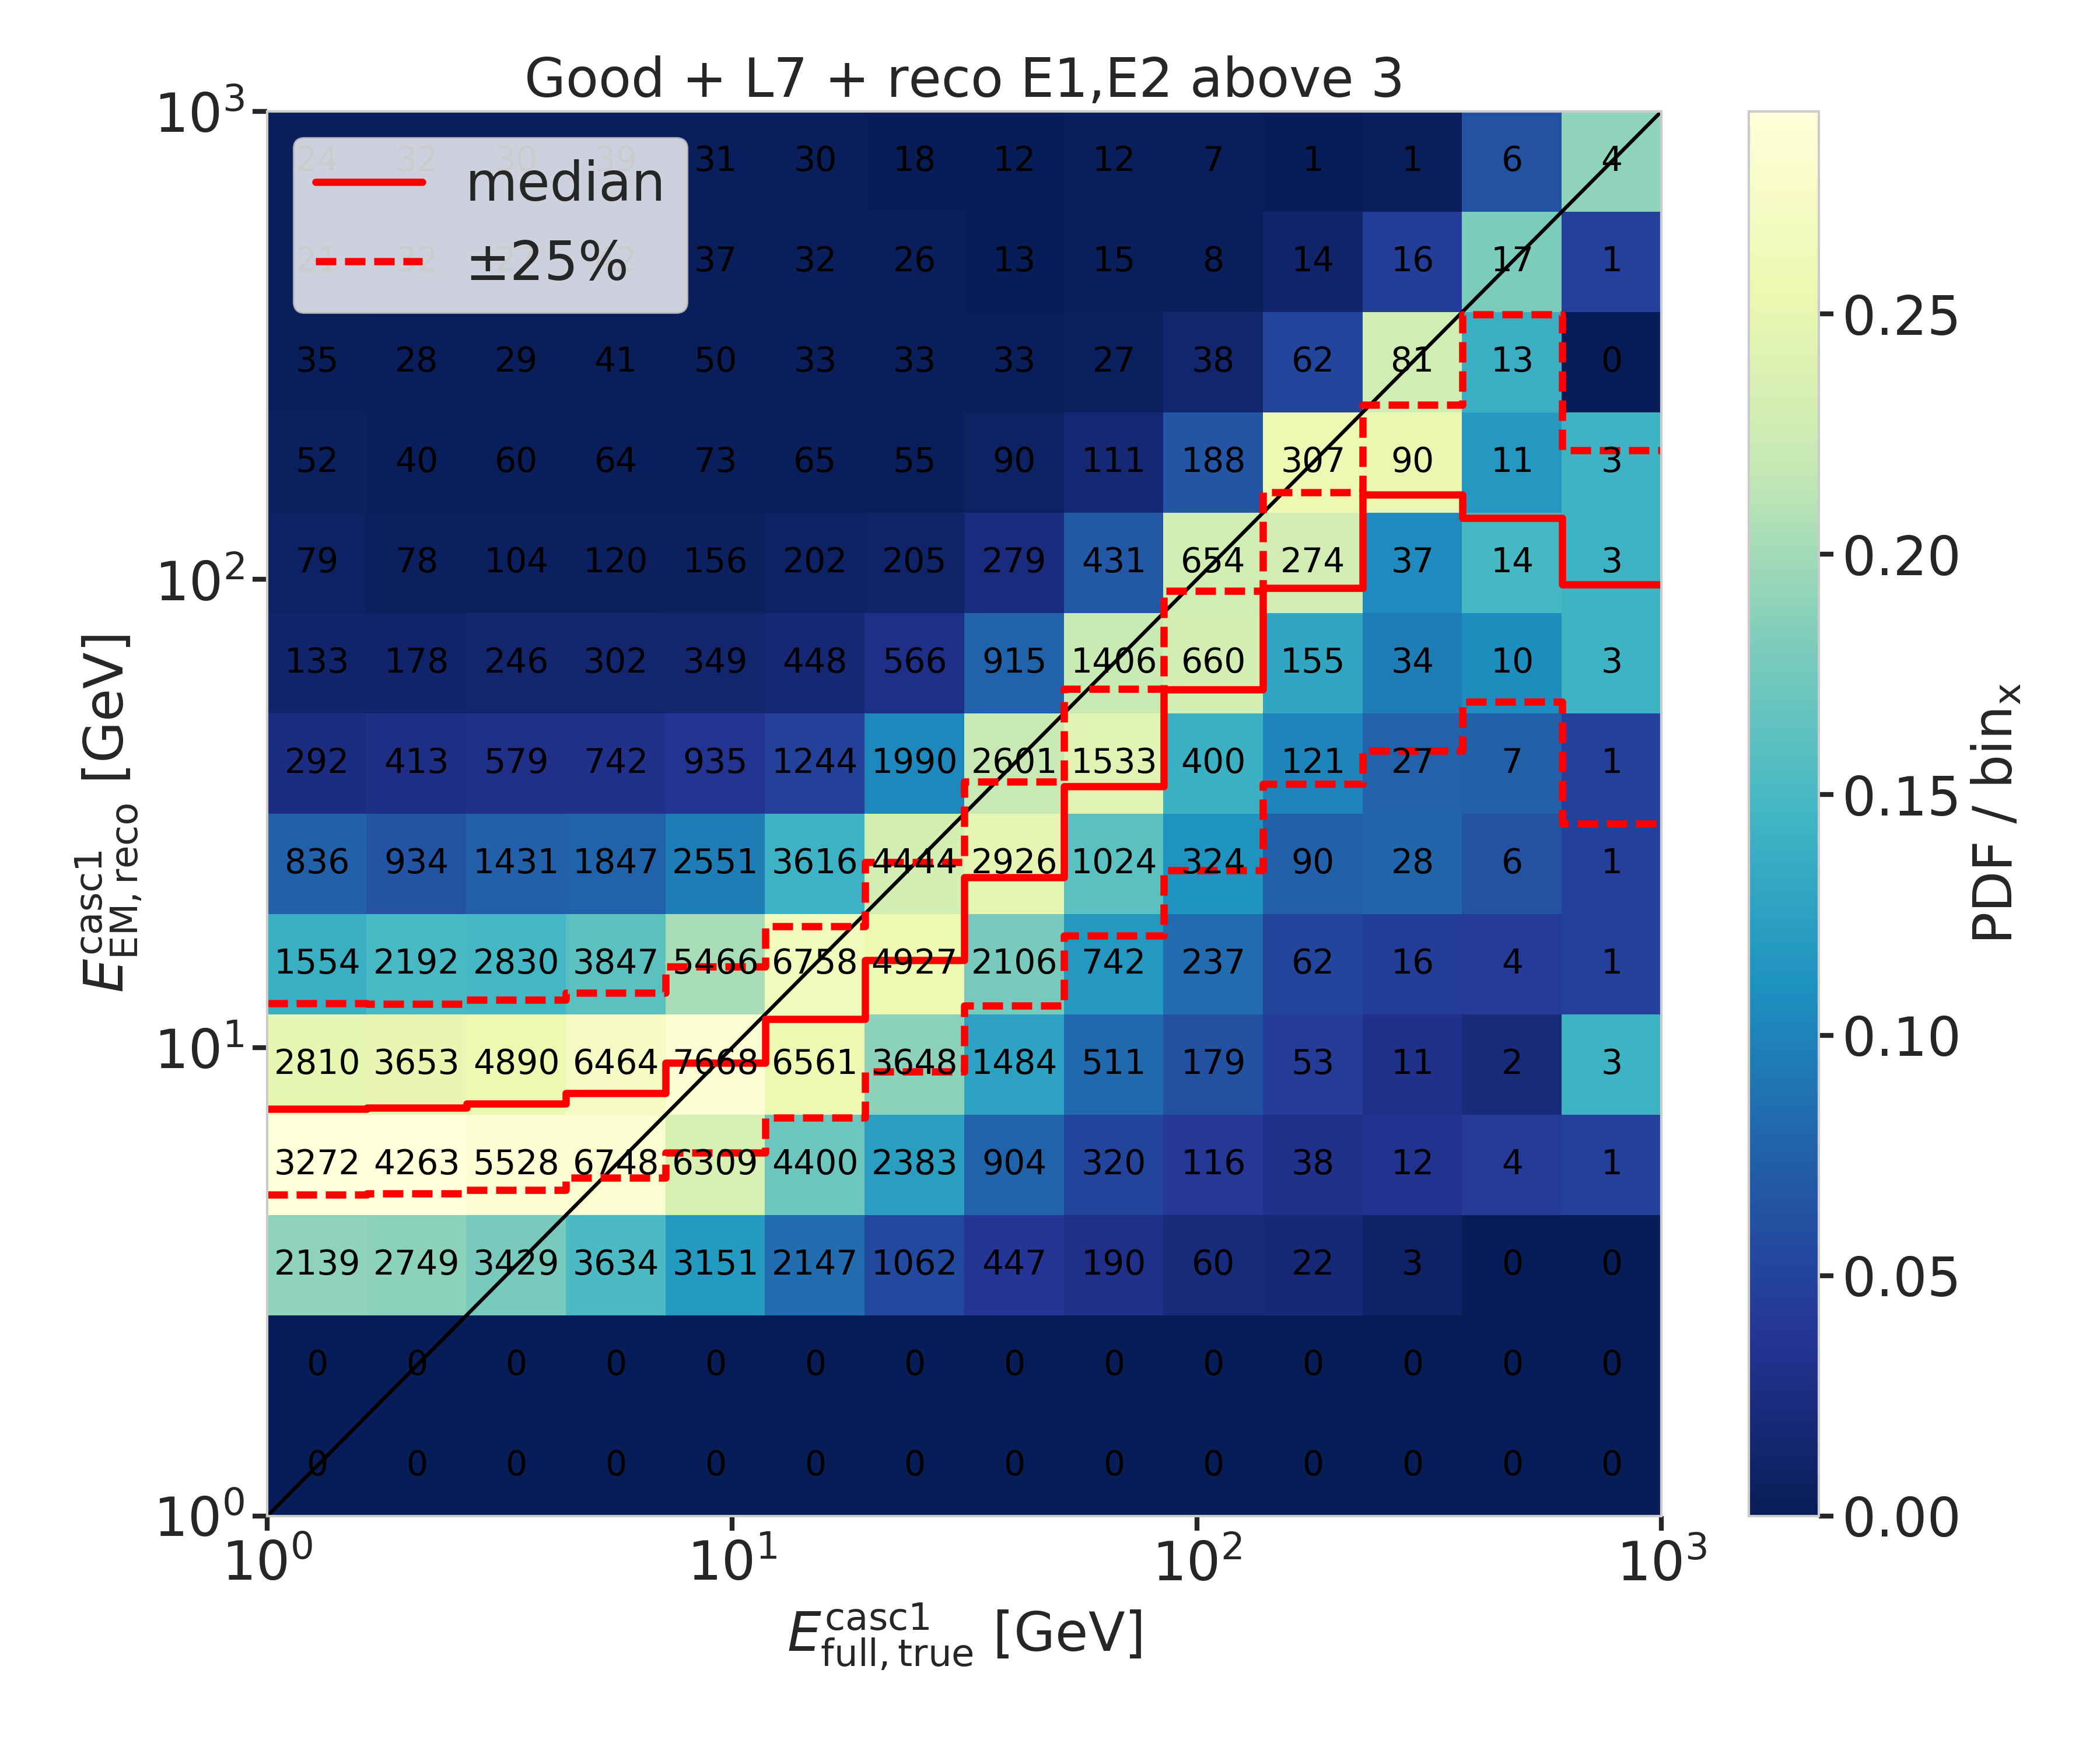
\includegraphics[width=0.49\linewidth]{figures/results/190607/resolutions/190607_millipede_level_no_NaNs_NEW_flipped_casc1_reco_energy_vs_casc1_true_energy_reco_above3_step_contours.png}
    \caption[Preliminary two-dimensional reconstructed versus true cascade energy resolutions]{Reconstructed (EM) energy versus true energy (full) energy for the first cascade (left) and second cascade (right). The color scale is according to the PDF in each vertical true energy slice, with the solid and dashed lines showing the median $\pm$\SI{25}{\percent} quantiles. The bin entries are shown as numbers.}
    \labfig{selected_routine_2d_energy_results}
\end{figure*}

The histogram for the first cascade energy is shown on the left and above an energy of $\sim$\SI{10}{\gev} the reconstruction performs well, with the median being parallel to the diagonal and the spread being small. Below this energy the reconstruction is over-estimating the true energy
% , which is a known effect in IceCube, where the reconstruction is biased towards higher energies around the energy detection threshold
, because events that enter the sample are events with an over fluctuation in their light deposition, which makes them pass into the selection and being reconstructible in the first place.

For the second cascade the overall behavior is similar, only that the energy where the reconstruction starts to perform well is higher around $\sim$\SI{20}{\gev}. The spread around the median is also larger and starts to expand a lot above \SI{200}{\gev}, where the statistics are lower as can be seen from the bin counts. It is also very apparent that the majority of events have a lower true energy in the second cascade, peaking between \SIrange[range-phrase=~and~]{1}{20}{\gev}. This can be seen by the indicated bin counts in the right part of \reffig{selected_routine_2d_energy_results}.

For both cascade resolutions the effect of the reconstruction being biased towards lower values can be seen. This is due to the comparison of the full true energy to the reconstructed EM energy as mentioned before.


\subsubsection{Length Resolutions} \labsec{190607_length_resolutions}

The decay length resolution is also investigated by looking at the two-dimensional histogram, where the reconstructed decay length is plotted versus the true decay length. The left part of \reffig{selected_routine_2d_length_results} shows the distributions after the same selection criteria from \refsec{190607_energy_resolutions} are applied. It can be observed that for short true lengths the reconstruction is over-estimating the length, while for long true lengths the reconstruction is strongly under-estimating the length. There is a region between true lengths of \SIrange[range-phrase=~and~]{20}{80}{\meter} where the median reconstruction is almost unbiased, but the \SI{50}{\percent} interquartile range is large and increasing from $\sim$\SI{50}{\meter} to $\sim$\SI{70}{\meter} with true decay lengths.

\begin{figure*}[h]
    \centering
    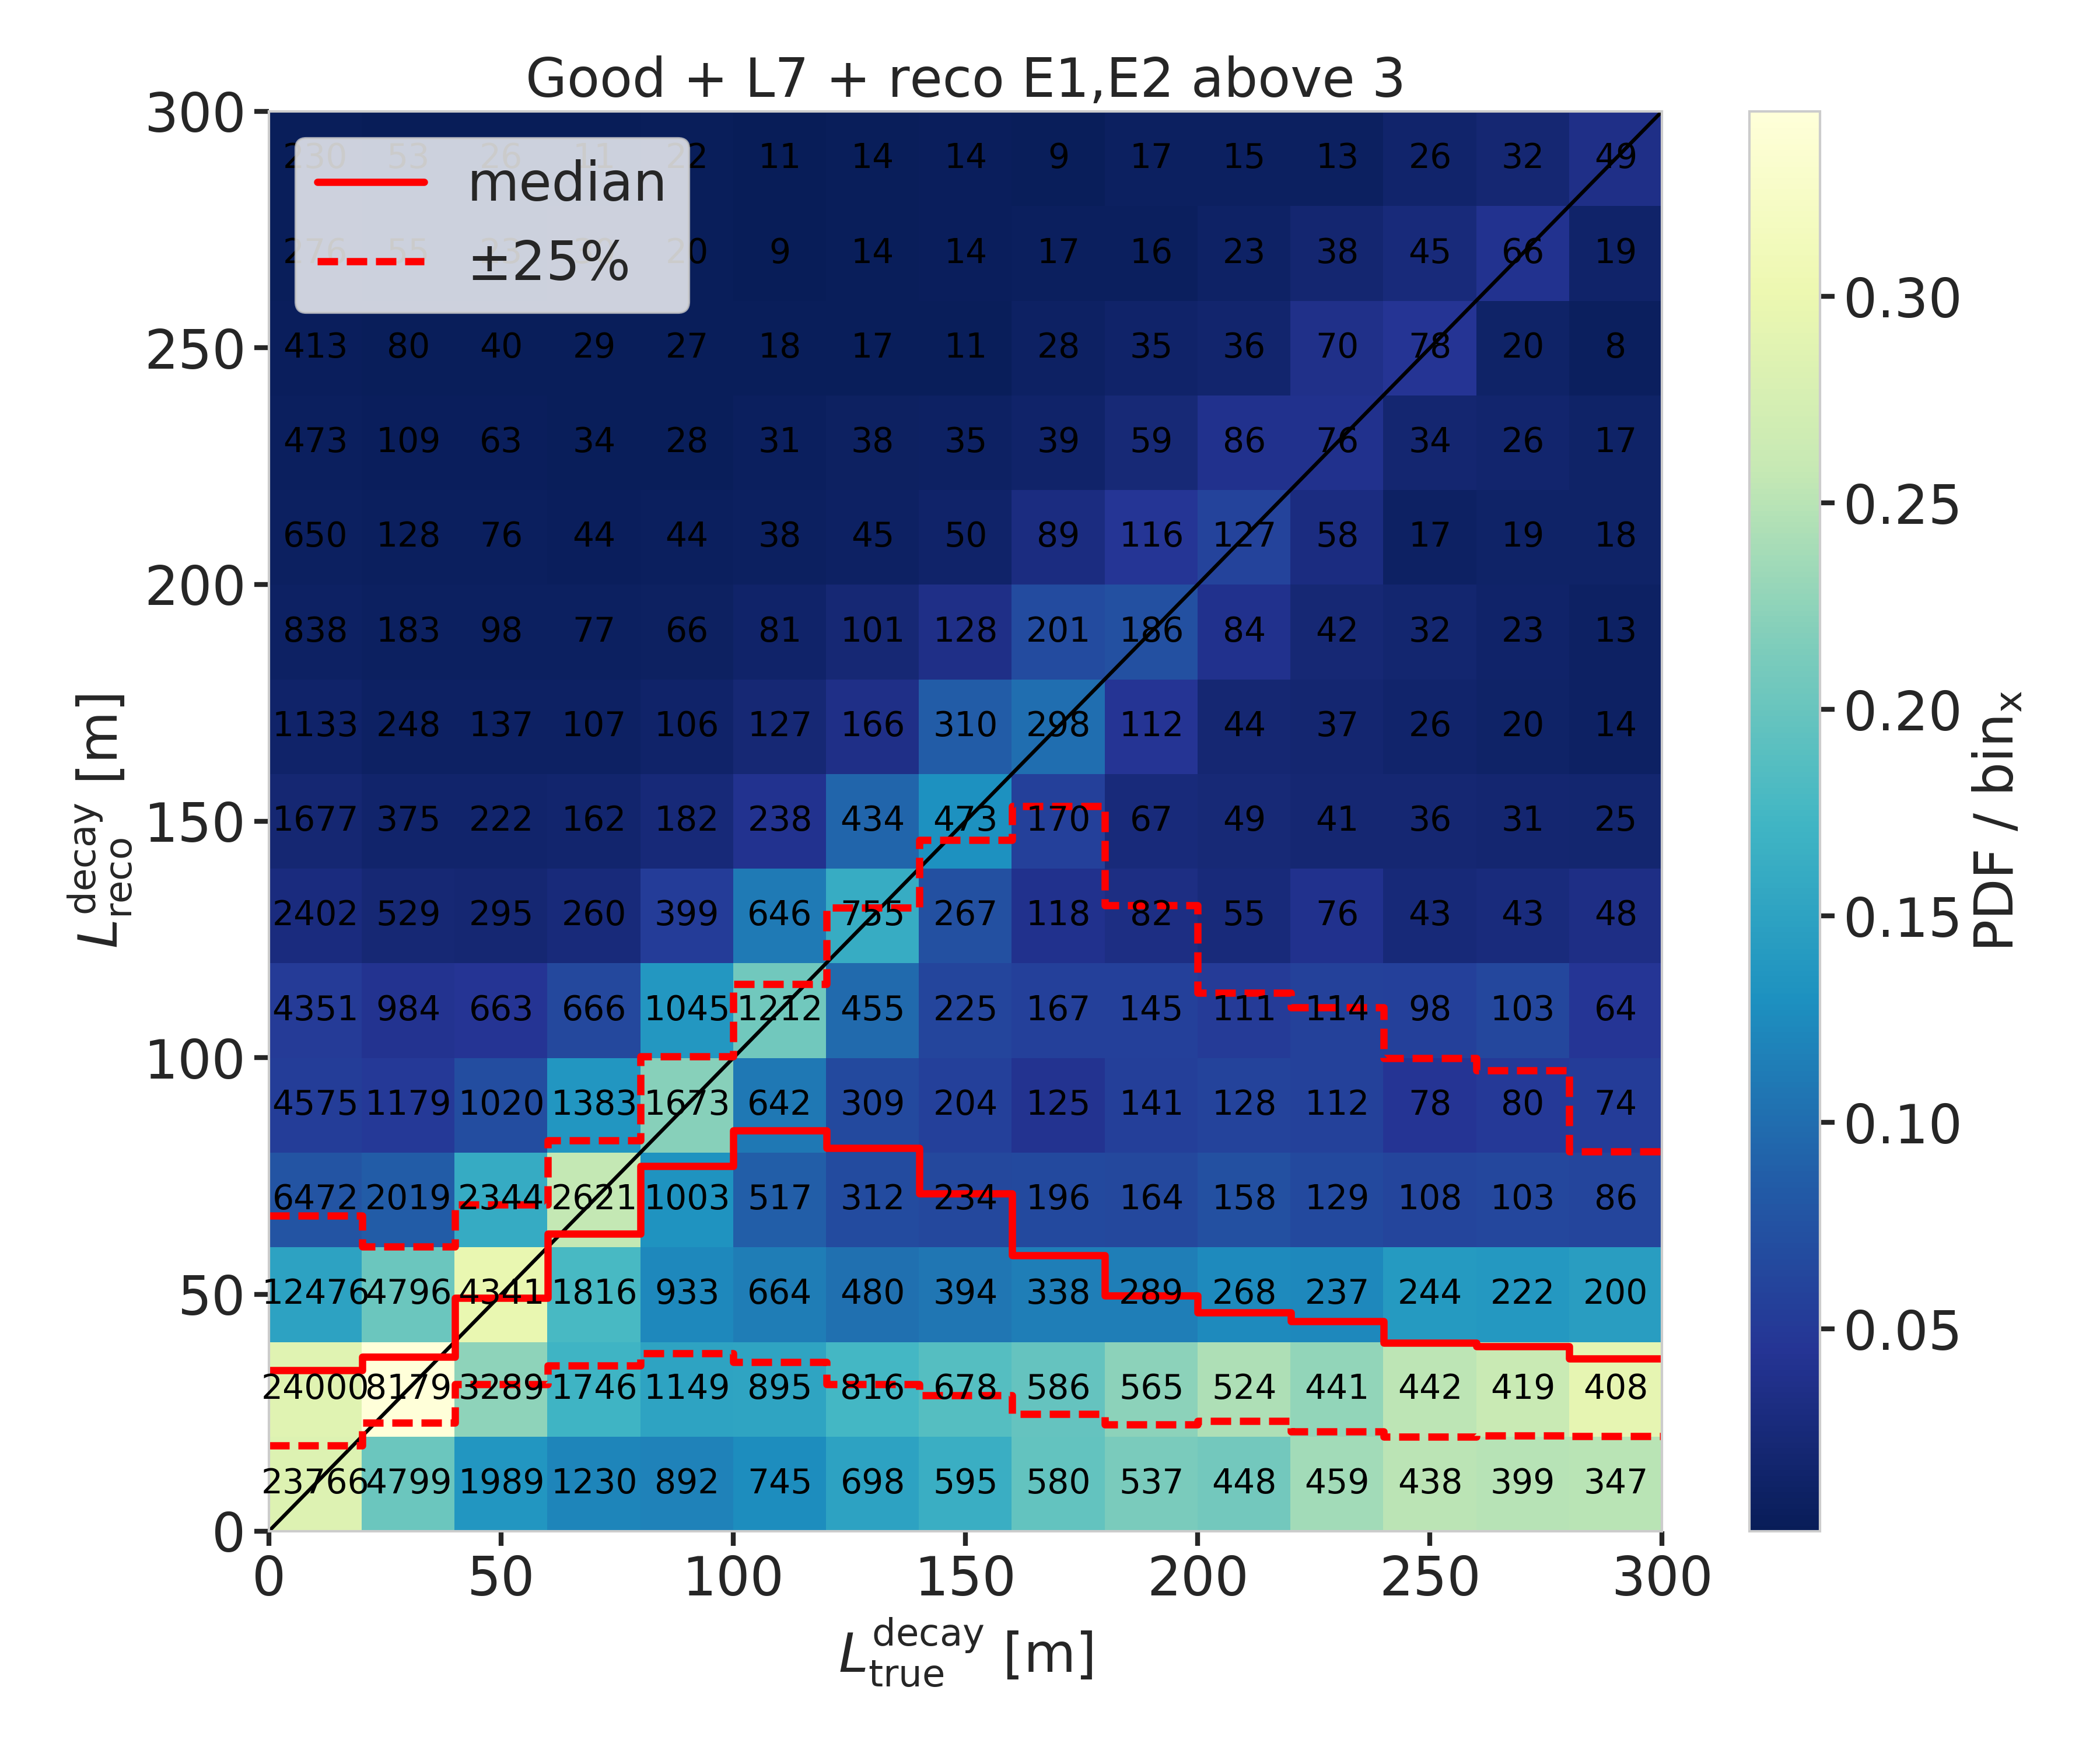
\includegraphics[width=0.49\linewidth]{figures/results/190607/resolutions/190607_millipede_level_no_NaNs_NEW_flipped_reco_decayL_vs_true_decayL_reco_above3_step_contours.png}
    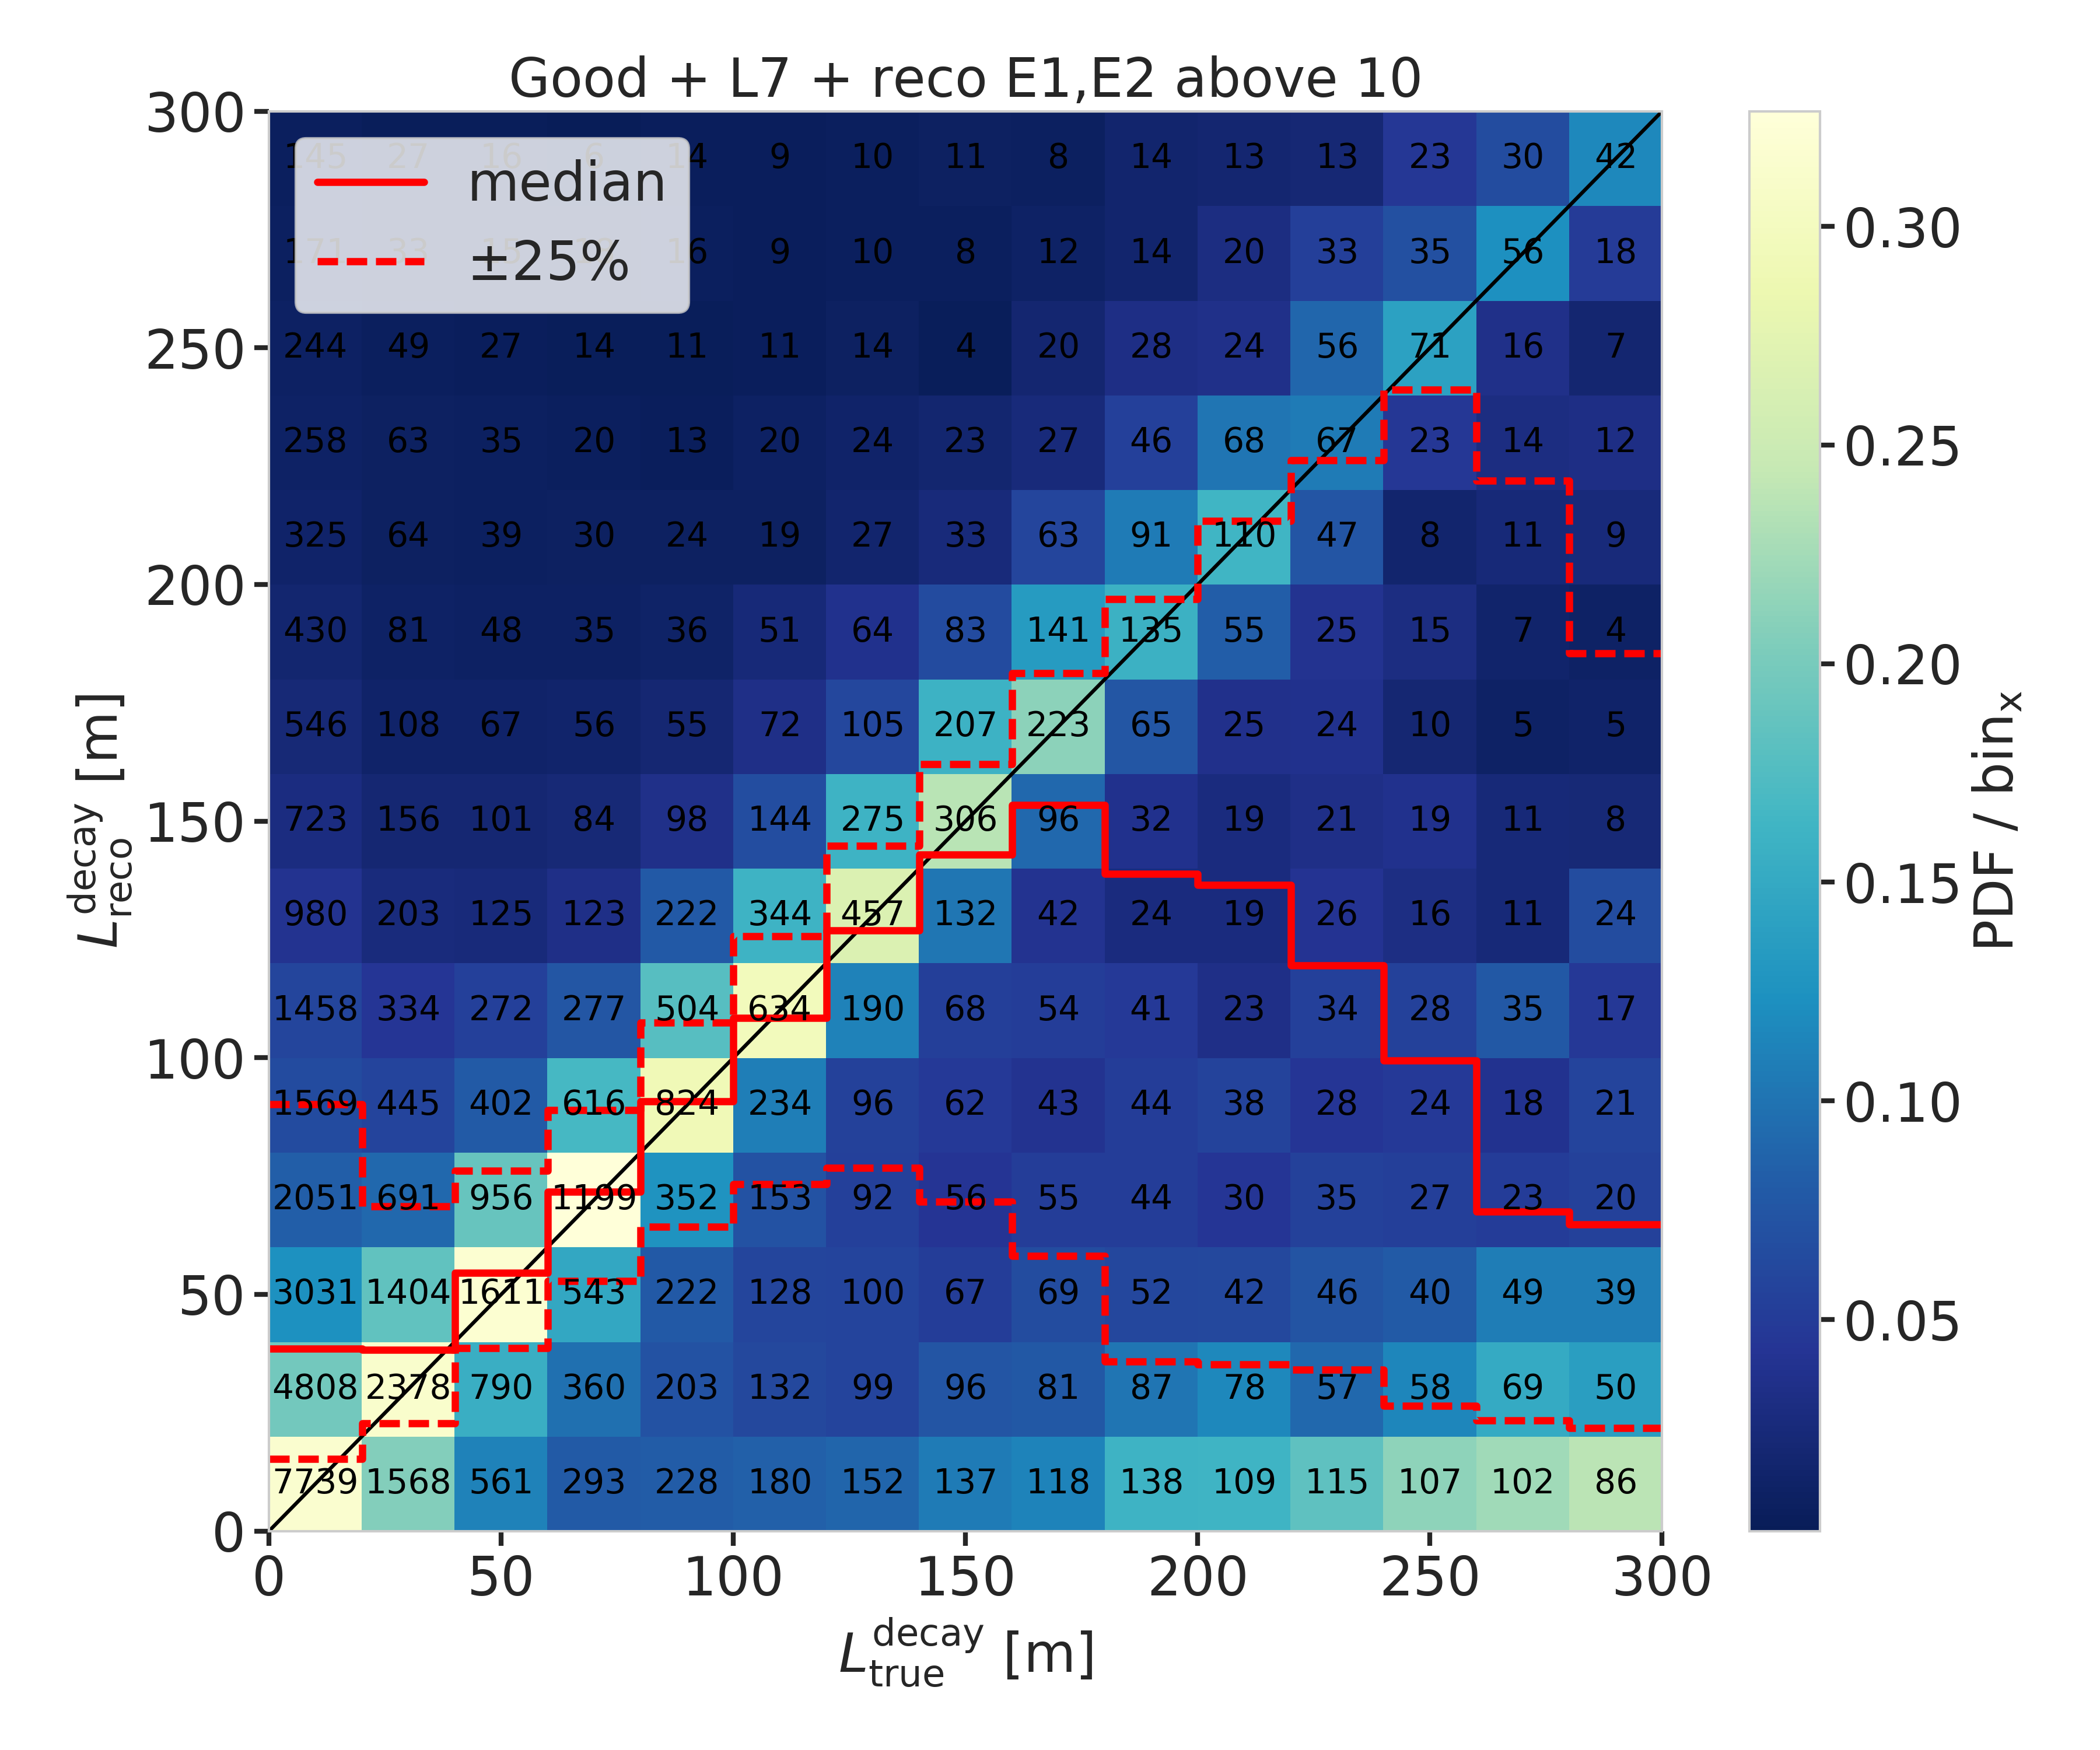
\includegraphics[width=0.49\linewidth]{figures/results/190607/resolutions/190607_millipede_level_no_NaNs_NEW_flipped_reco_decayL_vs_true_decayL_reco_above10_step_contours.png}
    \caption[Preliminary two-dimensional reconstructed versus true decay length resolutions]{Reconstructed decay length versus true decay length for $\sim$\SI{3}{\gev} (left) and $\sim$\SI{10}{\gev} (right) minimum reconstructed cascade energies. The color scale is according to the PDF in each vertical true length slice, with the solid and dashed lines showing the median $\pm$\SI{25}{\percent} quantiles. The bin entries are shown as numbers.}
    \labfig{selected_routine_2d_length_results}
\end{figure*}
\todo{blow up figures to make better visible? (ORANGE)}

The over-estimation at small true lengths can be explained by multiple factors, one being that the shortest DOM spacing is $\sim$\SI{7}{\meter}, vertically for DeepCore strings, but mostly larger than that, so resolving lengths below this is very complicated, and the reconstruction tends to be biased towards estimating the length around where the light was observed.
% Another reason is a similar argument to why the energies are over-estimated at small true values, namely that events that passed the selection and were reconstructed in those cases, probably have an over fluctuation in light deposition, extending further out from the vertices, so the reconstructed length is larger.
Additionally, approaching a length of 0.0, the reconstructed length will of course always be a one-sided distribution, because the lengths have to be positive.

The under-estimation at large true lengths is more puzzling, and it seems like the distribution becomes bimodal in the reconstructed lengths, with one population around the diagonal, meaning that they are properly reconstructed, and another population at very short reconstructed lengths, which are badly reconstructed. Above \SI{150}{\meter} the badly reconstructed population starts to dominate, and the median resolution drops off strongly. The assumption is that for these events, only one cascade was observed with enough light to be reconstructed, and the reconstruction describes the one observed cascade in two parts, separated by a short distance, driven by similar factors as mentioned before. A quick check to confirm whether this is the case, was to increase the selection criteria to minimum reconstructed cascade energies of \SI{10}{\gev}, which is shown in the right part of \reffig{selected_routine_2d_length_results}. It can be seen that the median resolution is already much better, aligning with the expectation between \SIrange[range-phrase=~and~]{40}{160}{\meter}. Judging from the median resolution and the spread in this range, there are very few events with an over-expectation in the energy, since both of them are aligning with the diagonal. Towards lower reconstructed lengths on the other hand, the spread is still very large, and above \SI{200}{\meter} the badly reconstructed population starts to dominate again.


\subsubsection{Badly Reconstructed Cascade Population}

\begin{figure}[h]
    % \centering
    % 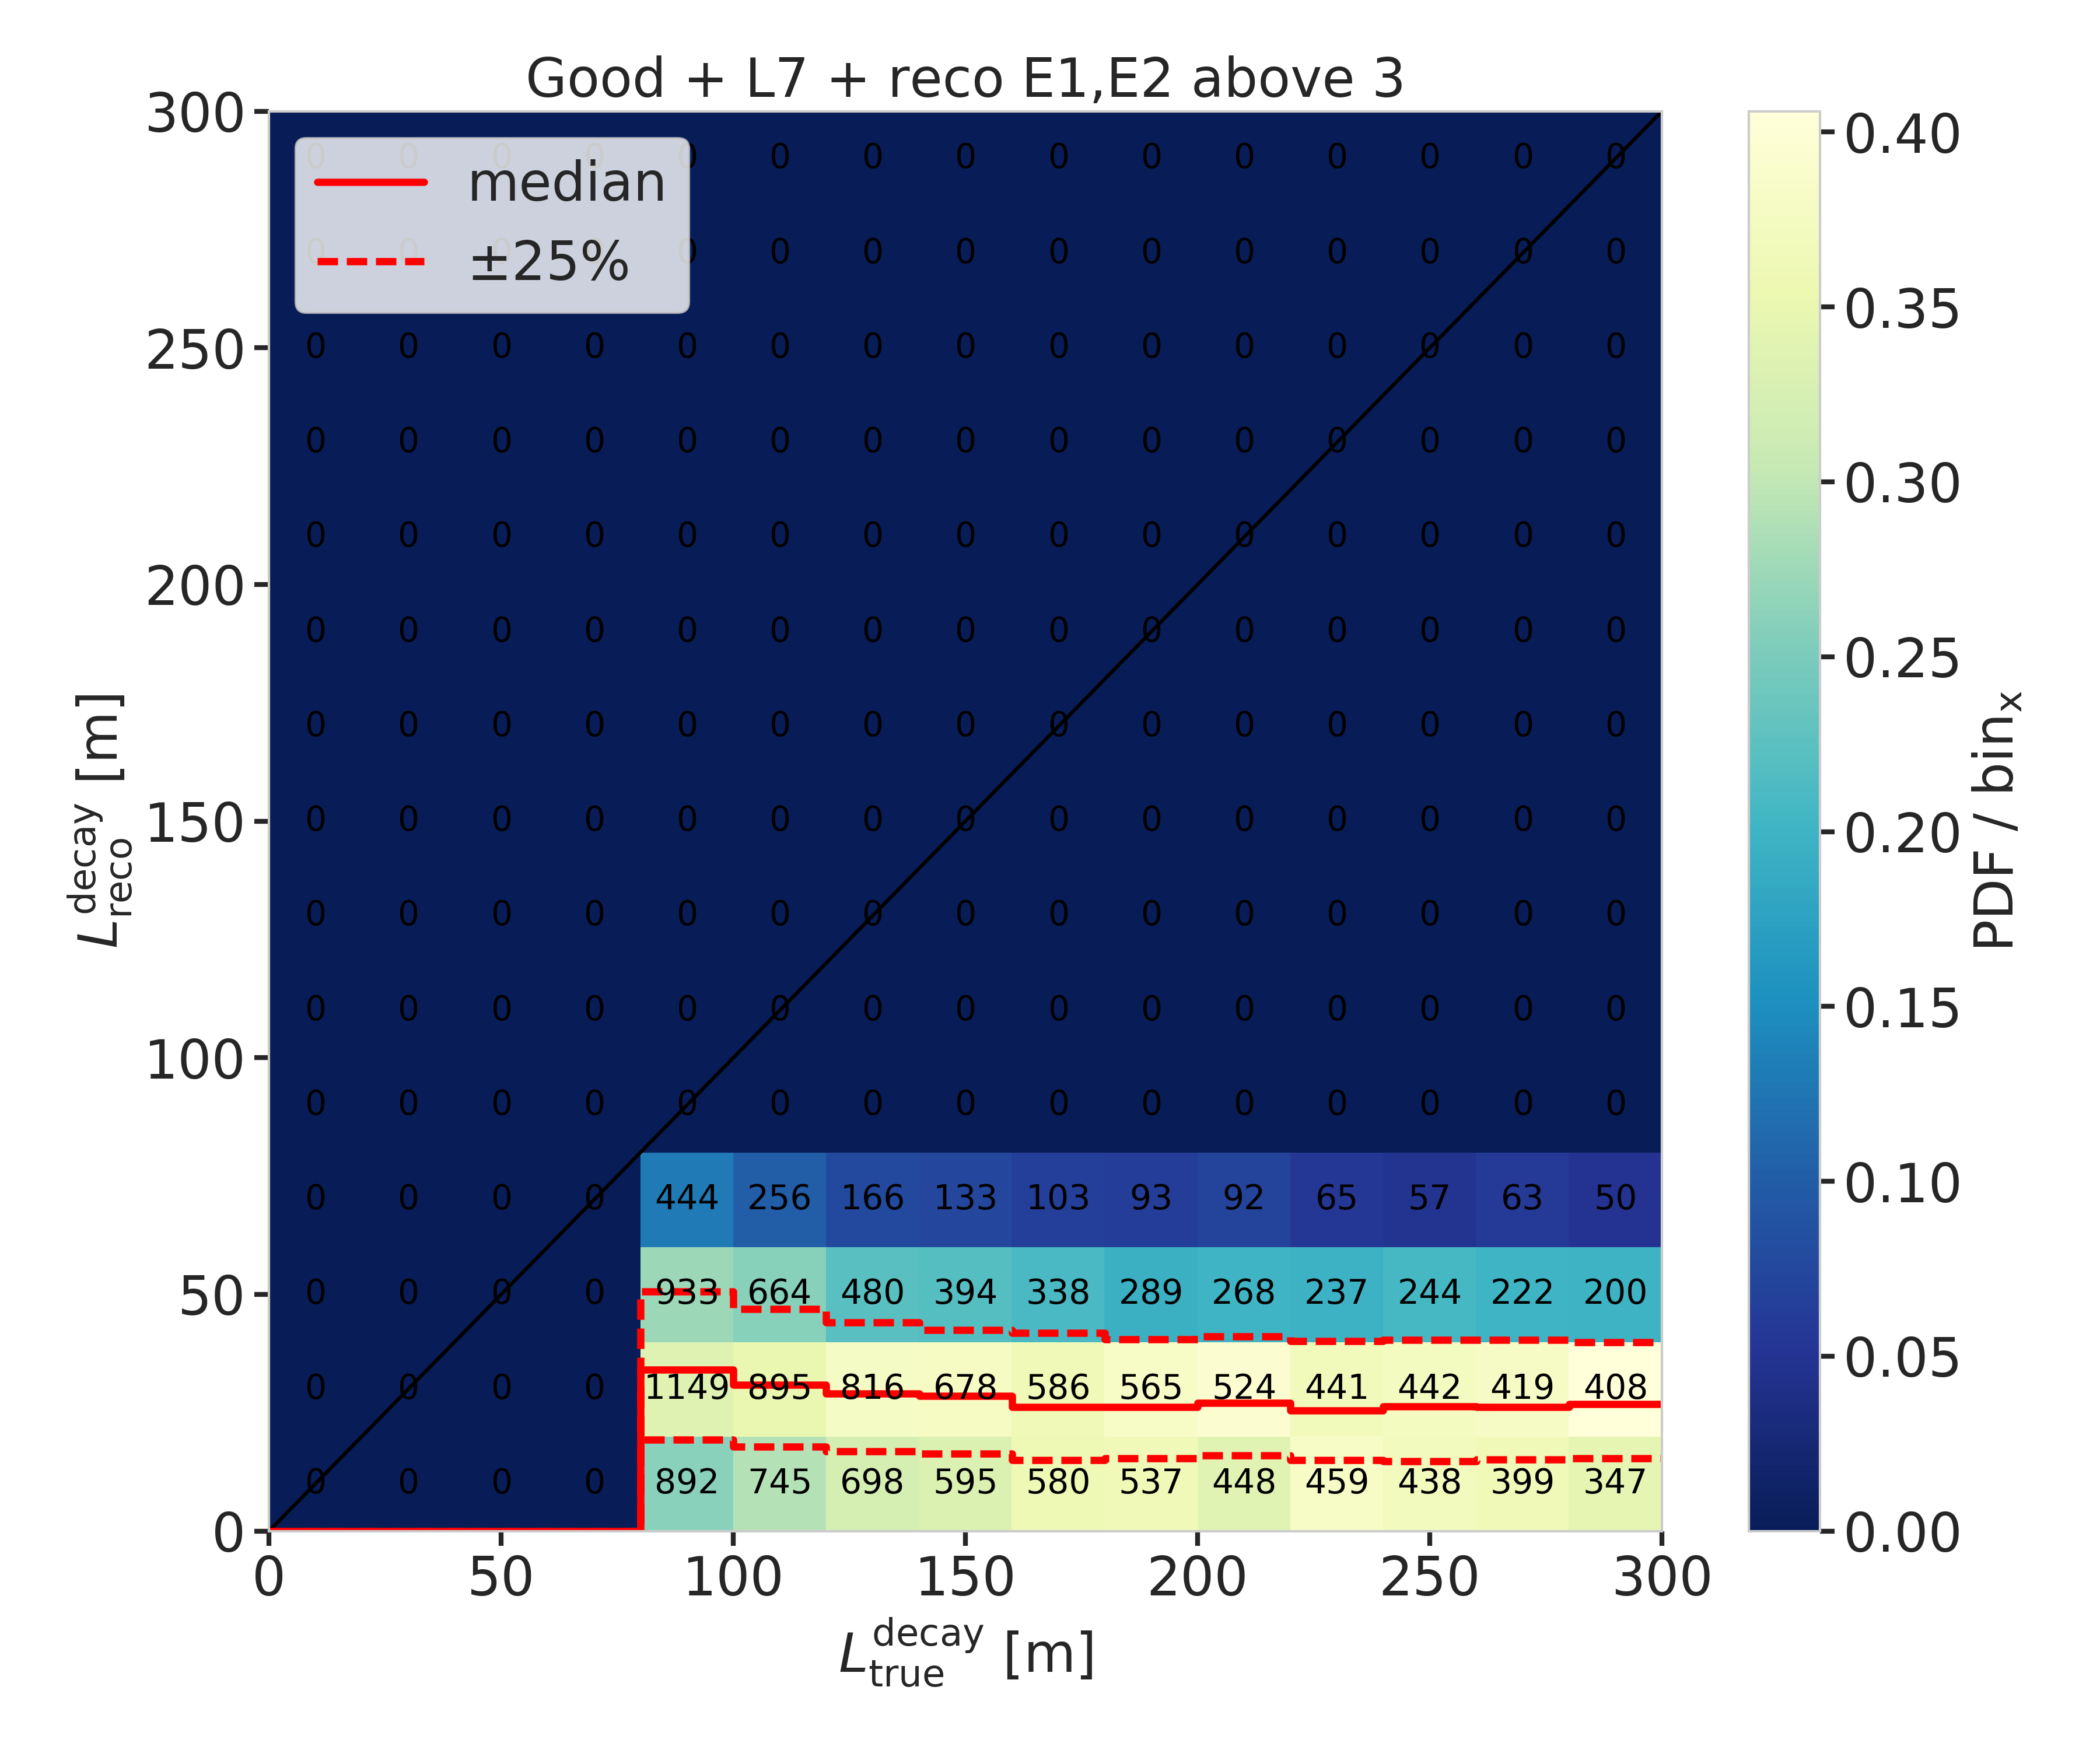
\includegraphics[width=0.49\linewidth]{figures/results/190607/second_population/190607_millipede_level_no_NaNs_NEW_flipped_reco_decayL_vs_true_decayL_reco_above3_population_in_step_contours.png}
    % 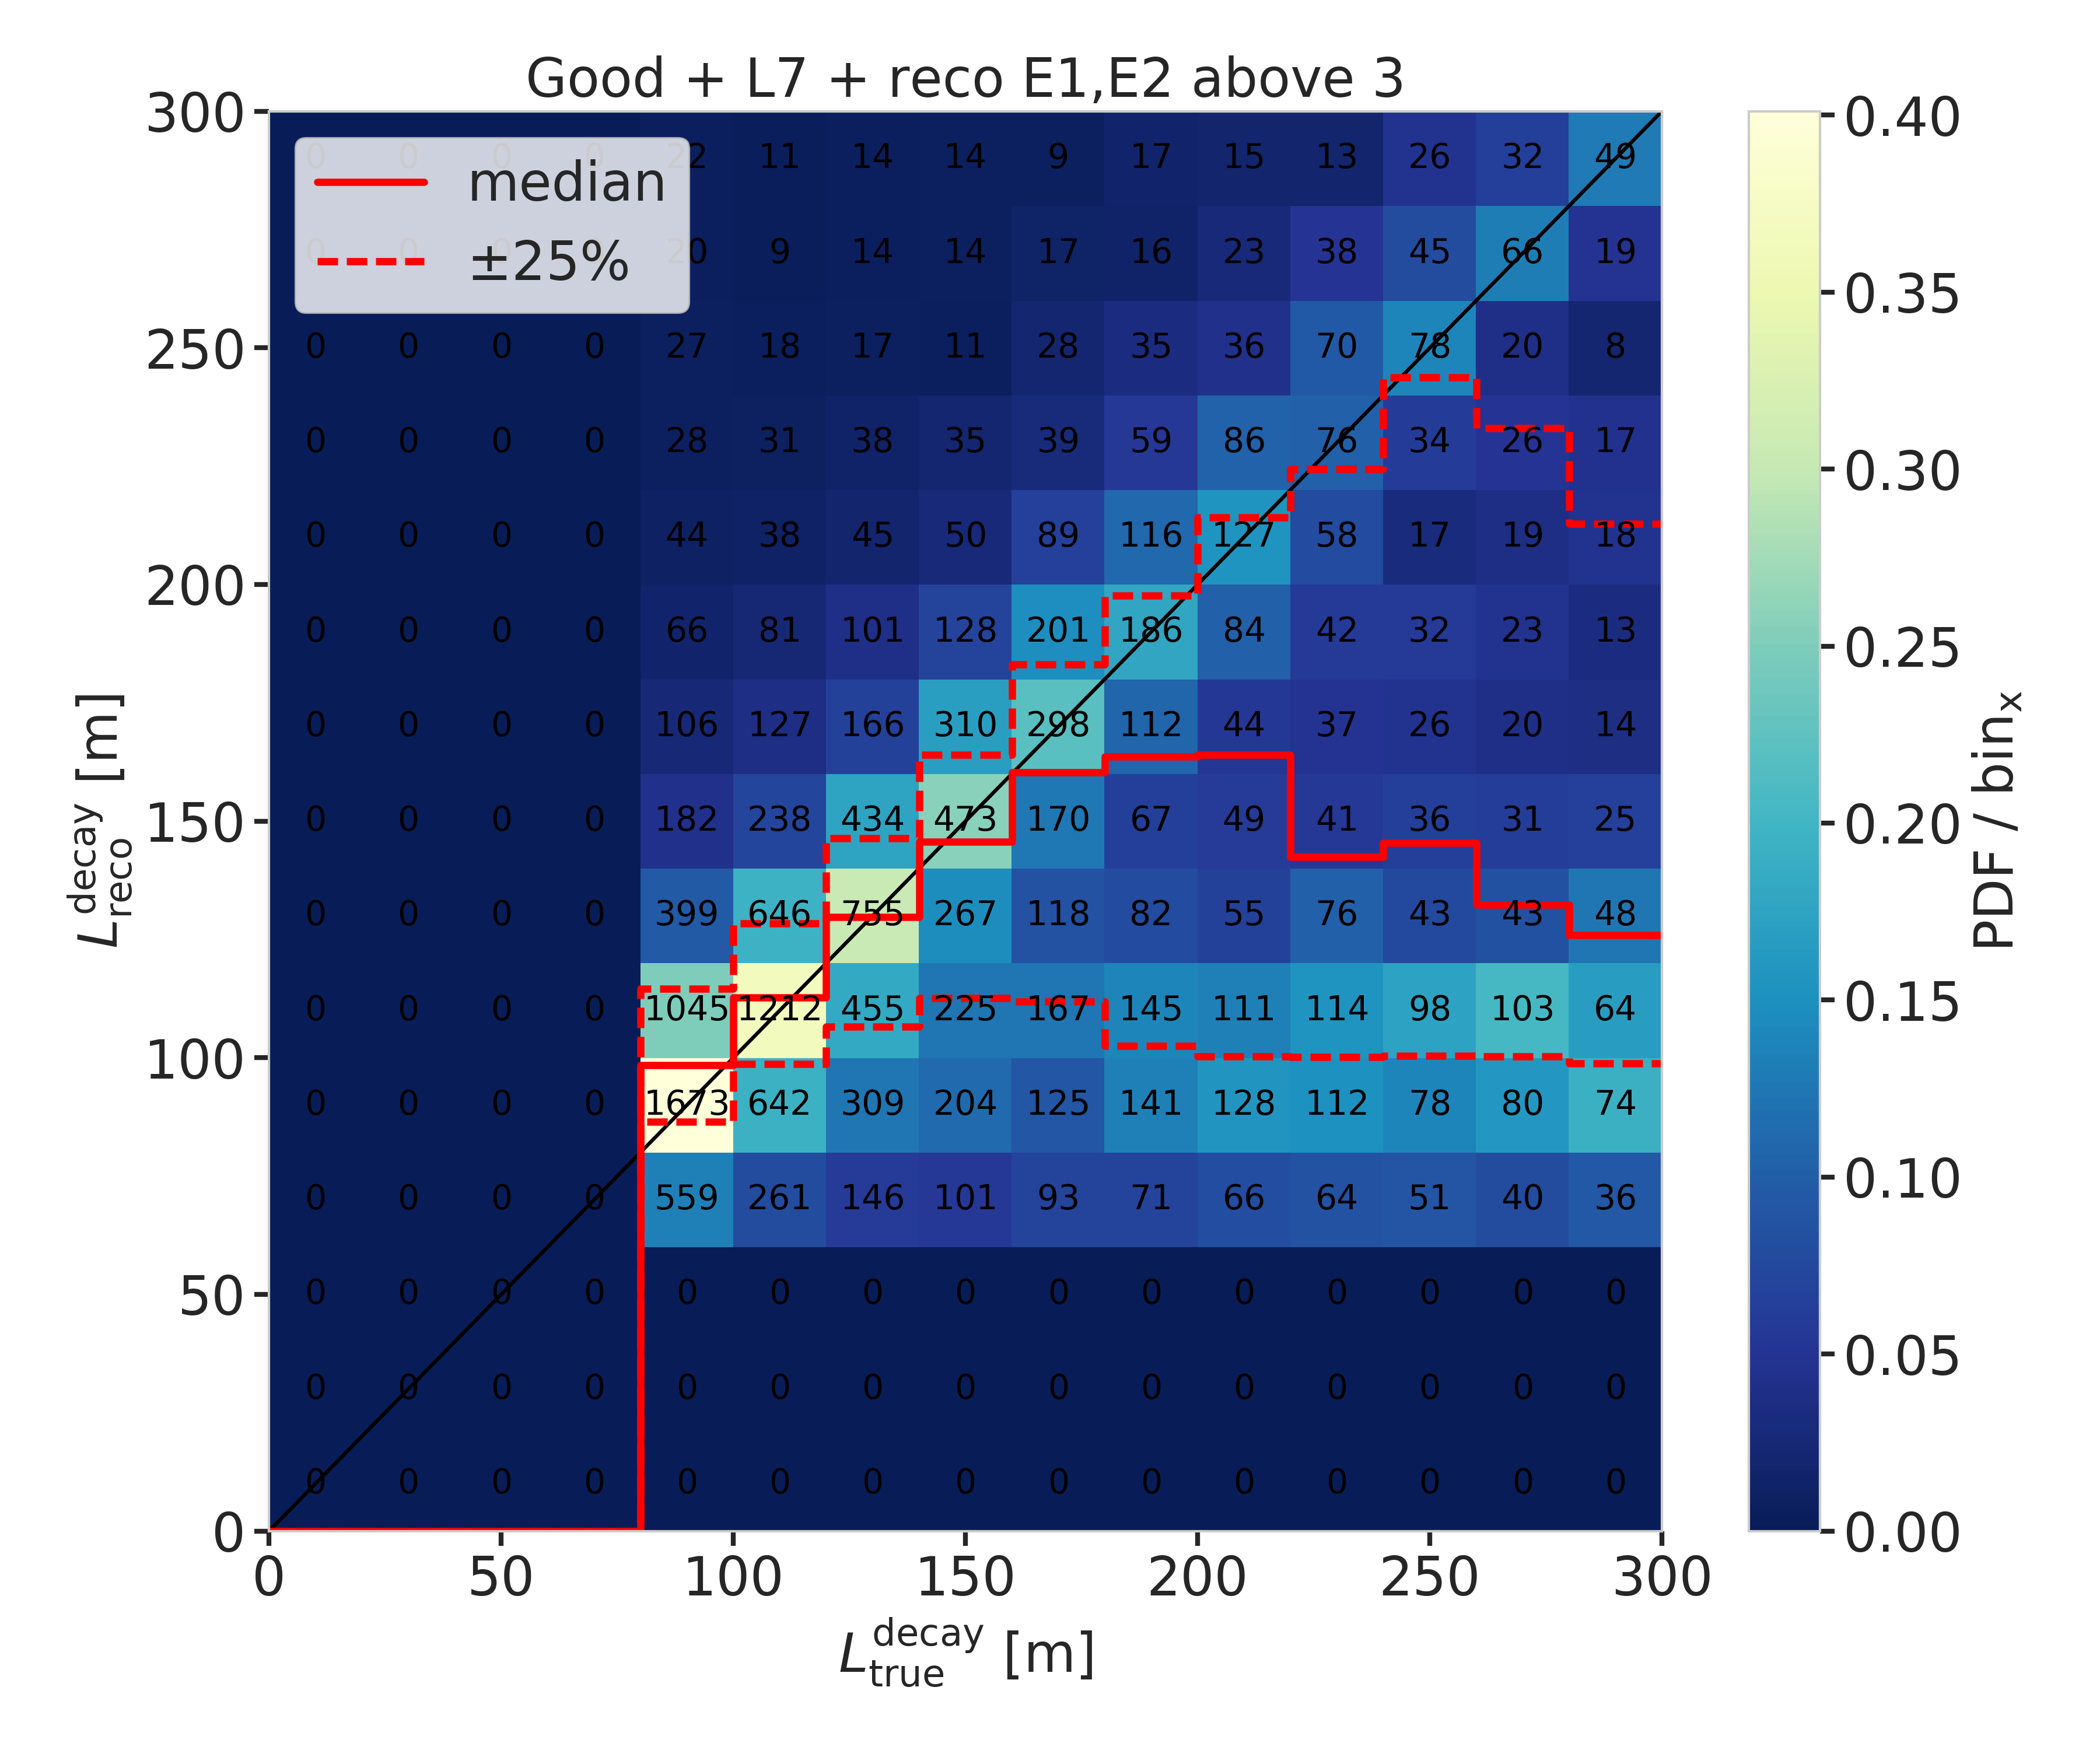
\includegraphics[width=0.49\linewidth]{figures/results/190607/second_population/190607_millipede_level_no_NaNs_NEW_flipped_reco_decayL_vs_true_decayL_reco_above3_population_out_step_contours.png}
    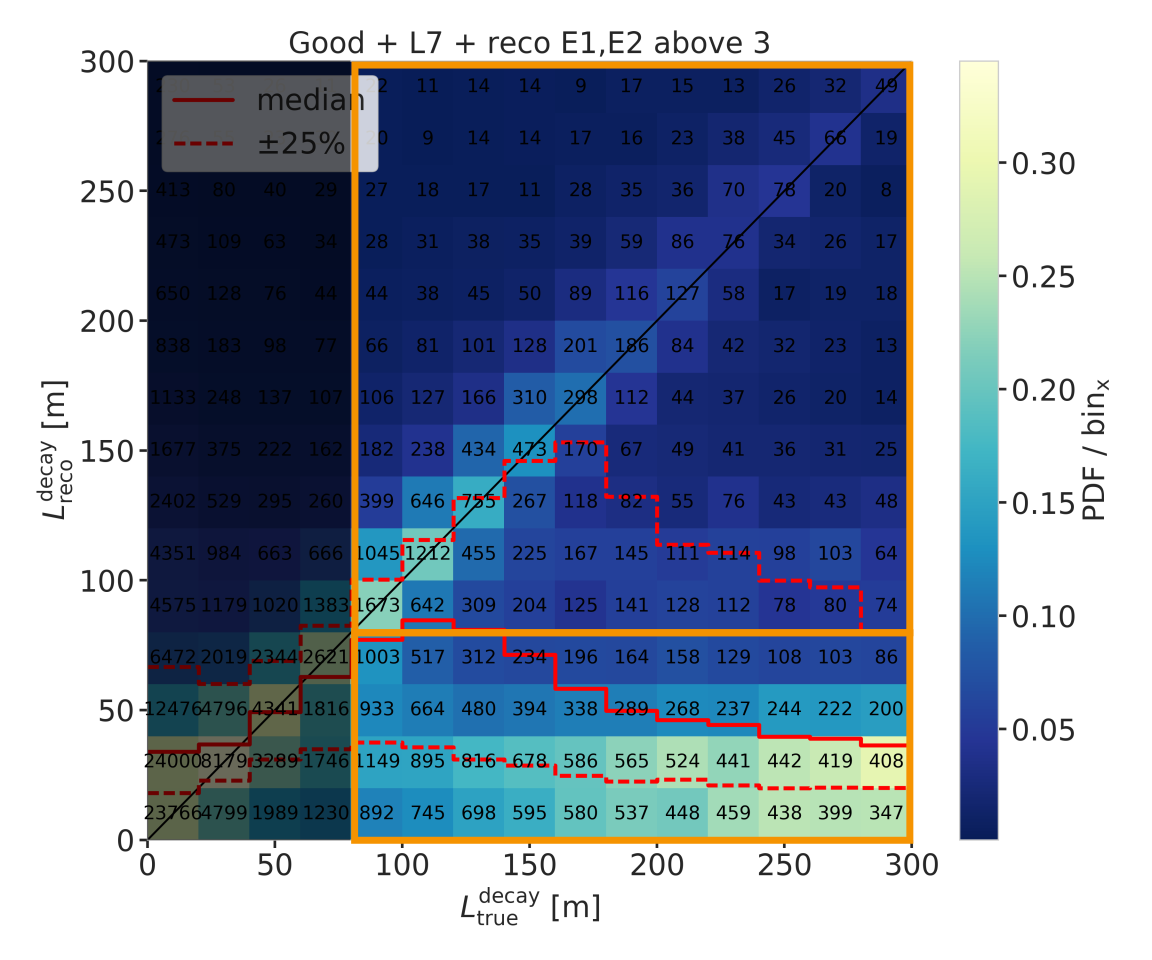
\includegraphics{figures/results/190607/second_population/190607_millipede_level_no_NaNs_NEW_flipped_reco_decayL_vs_true_decayL_reco_above3_step_contours_populations.png}
    \caption[]{}
    \labfig{true_energies_vs_true_length_populations_in_out}
\end{figure}
\todo{remake plot: no bin counts, blow up labels etc. margin possible? (RED)}
\todo{fix caption (RED)}

To investigate the badly reconstructed population further, a rough separation was made to find out what the cause of the difference is. It was already established that a larger reconstructed energy in both cascades, which is related to a larger true energy in form of more deposited light, leads to a better reconstruction in more events. To select the two populations, only events with true decay length larger than \SI{80}{\meter} are used as shown in \reffig{true_energies_vs_true_length_populations_in_out}, and the populations are split by the reconstructed decay length being larger or smaller than \SI{80}{\meter}. To investigate the difference between the two populations, several variables were compared to find the reason(s) for the bad reconstruction. 

The left part of \reffig{population_position_direction} shows the true horizontal distance of the second cascade from string 36. The distance is denoted as $\rho_{36}$ and is a very good proxy for the distance to the center of the detector, because string 36 is almost at the center. While the distributions looks very similar for the first cascade (not shown), for the second cascade the badly reconstructed population extends to larger values. Considering that the DeepCore strings are roughly inside a \SI{70}{\meter} radius from the center, and the next layer of IceCube strings is at a radius of \SI{125}{\meter}, this is a plausible explanation for a worse reconstruction, because for the badly reconstructed population the second cascades are more often in regions without DOMs, so less or no light is observed from them.

\begin{figure*}[h]
    \centering
    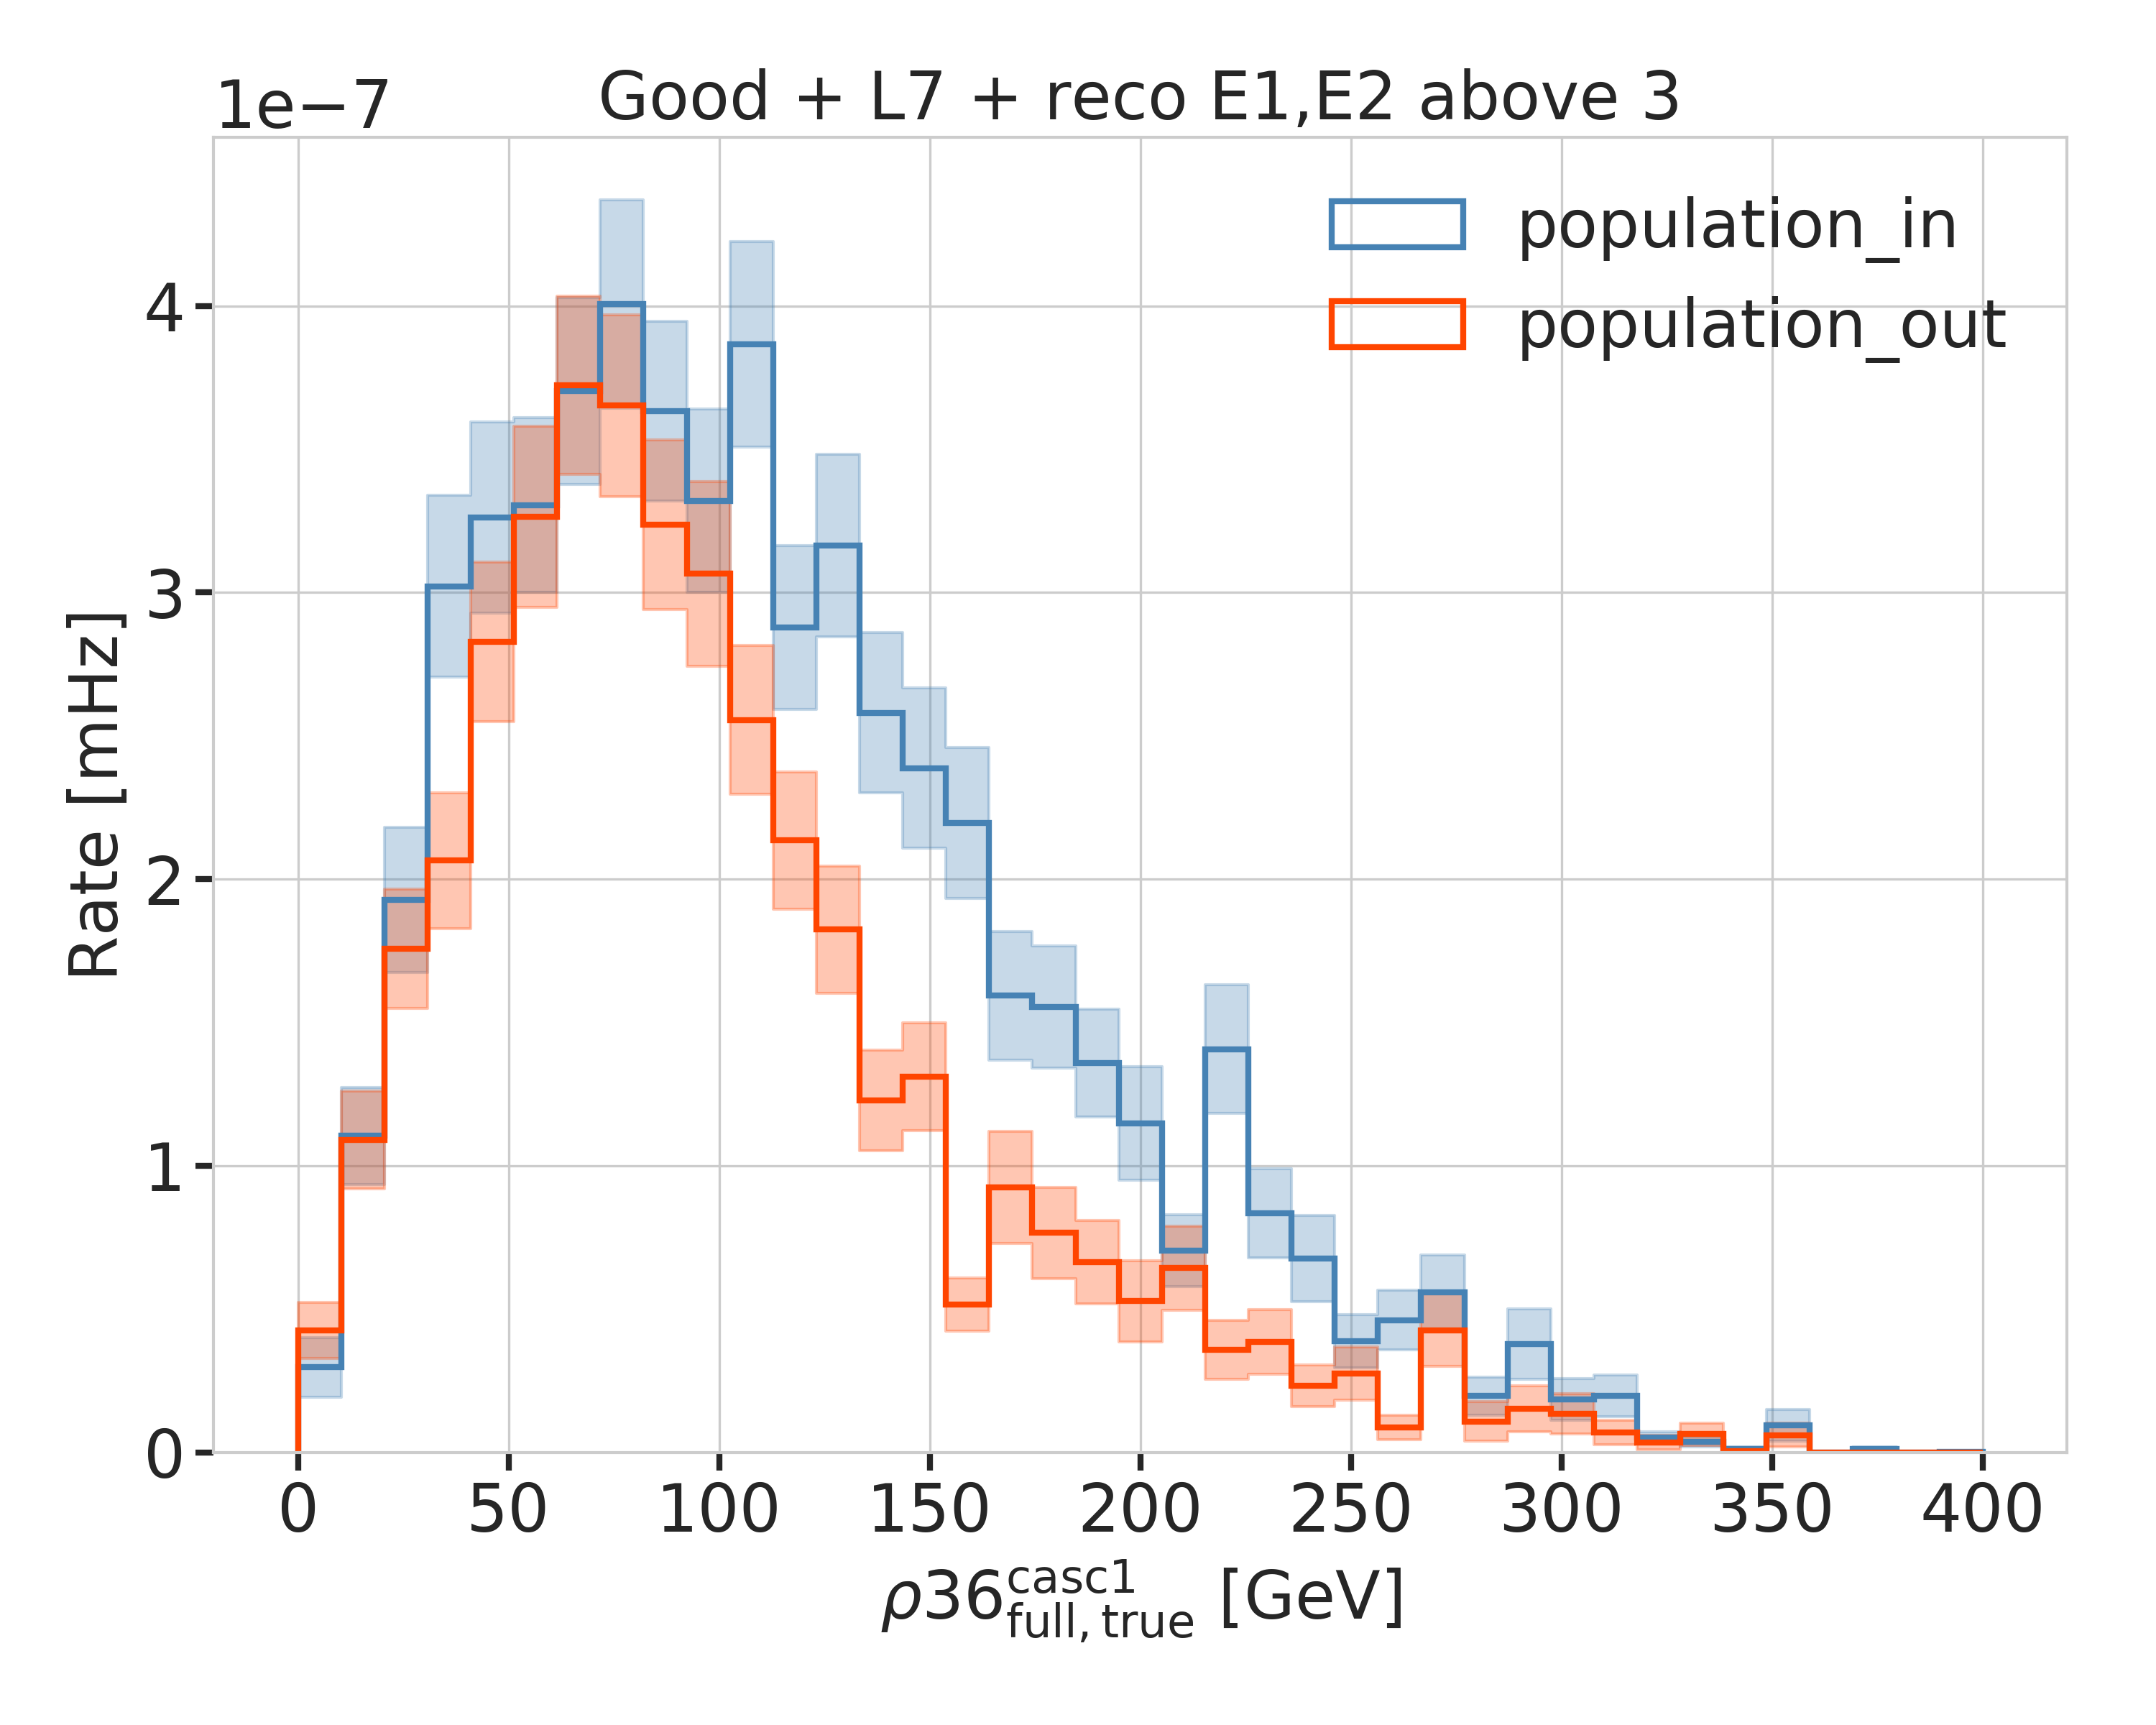
\includegraphics[width=0.49\linewidth]{figures/results/190607/second_population/casc1_rho36.png}
    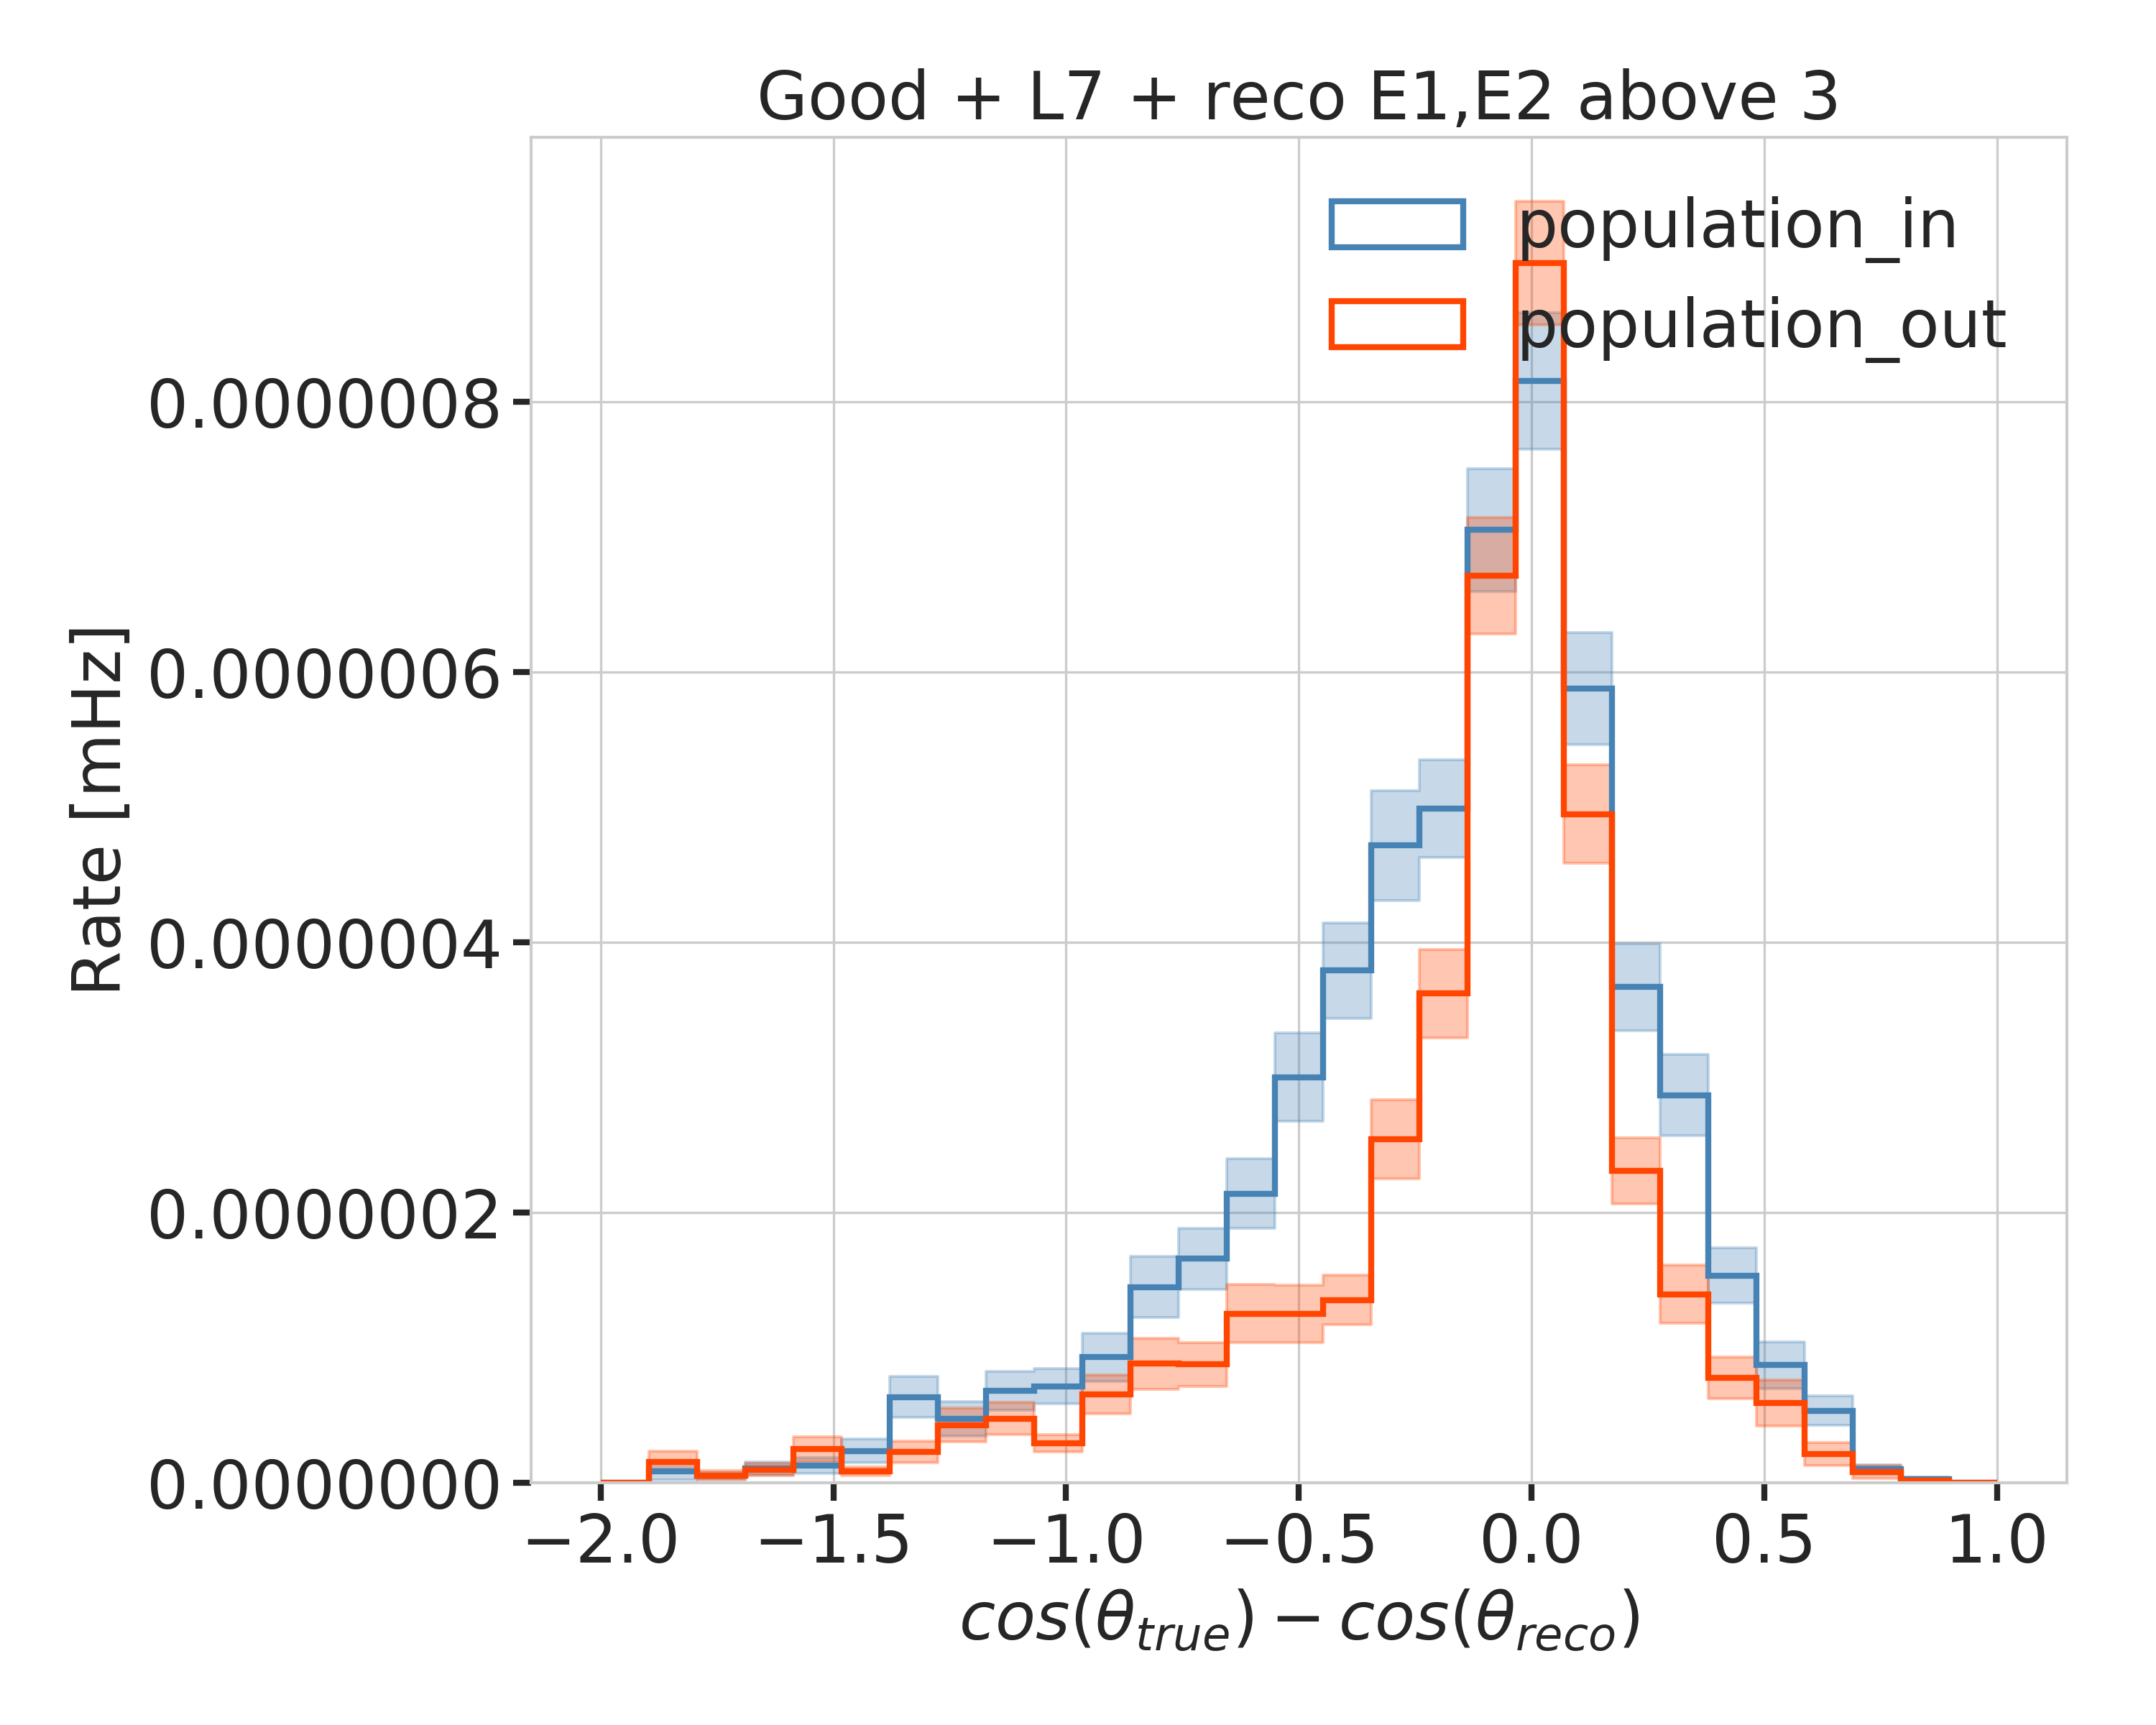
\includegraphics[width=0.49\linewidth]{figures/results/190607/second_population/reco_true_cos_zenith_error_populations.png}
    \caption[]{}
    \labfig{population_position_direction}
\end{figure*}
\todo{re-make normalized? (ORANGE)}
\todo{fix caption (RED)}

Another possible reason why the reconstruction underperforms could be that the initial seed direction itself was off and therefore one of the cascades cannot be found properly. Looking at the error of the cosine of the reconstructed zenith angle shown in the right of \reffig{population_position_direction}, we see that the badly reconstructed population has a larger error, and is less peaked around 0.0. This could be a hint that the direction is worse for the badly reconstructed population, which could be due to a bad seed direction, or just the result of one cascade not depositing enough light to be observed.

\begin{figure*}[h]
    \centering
    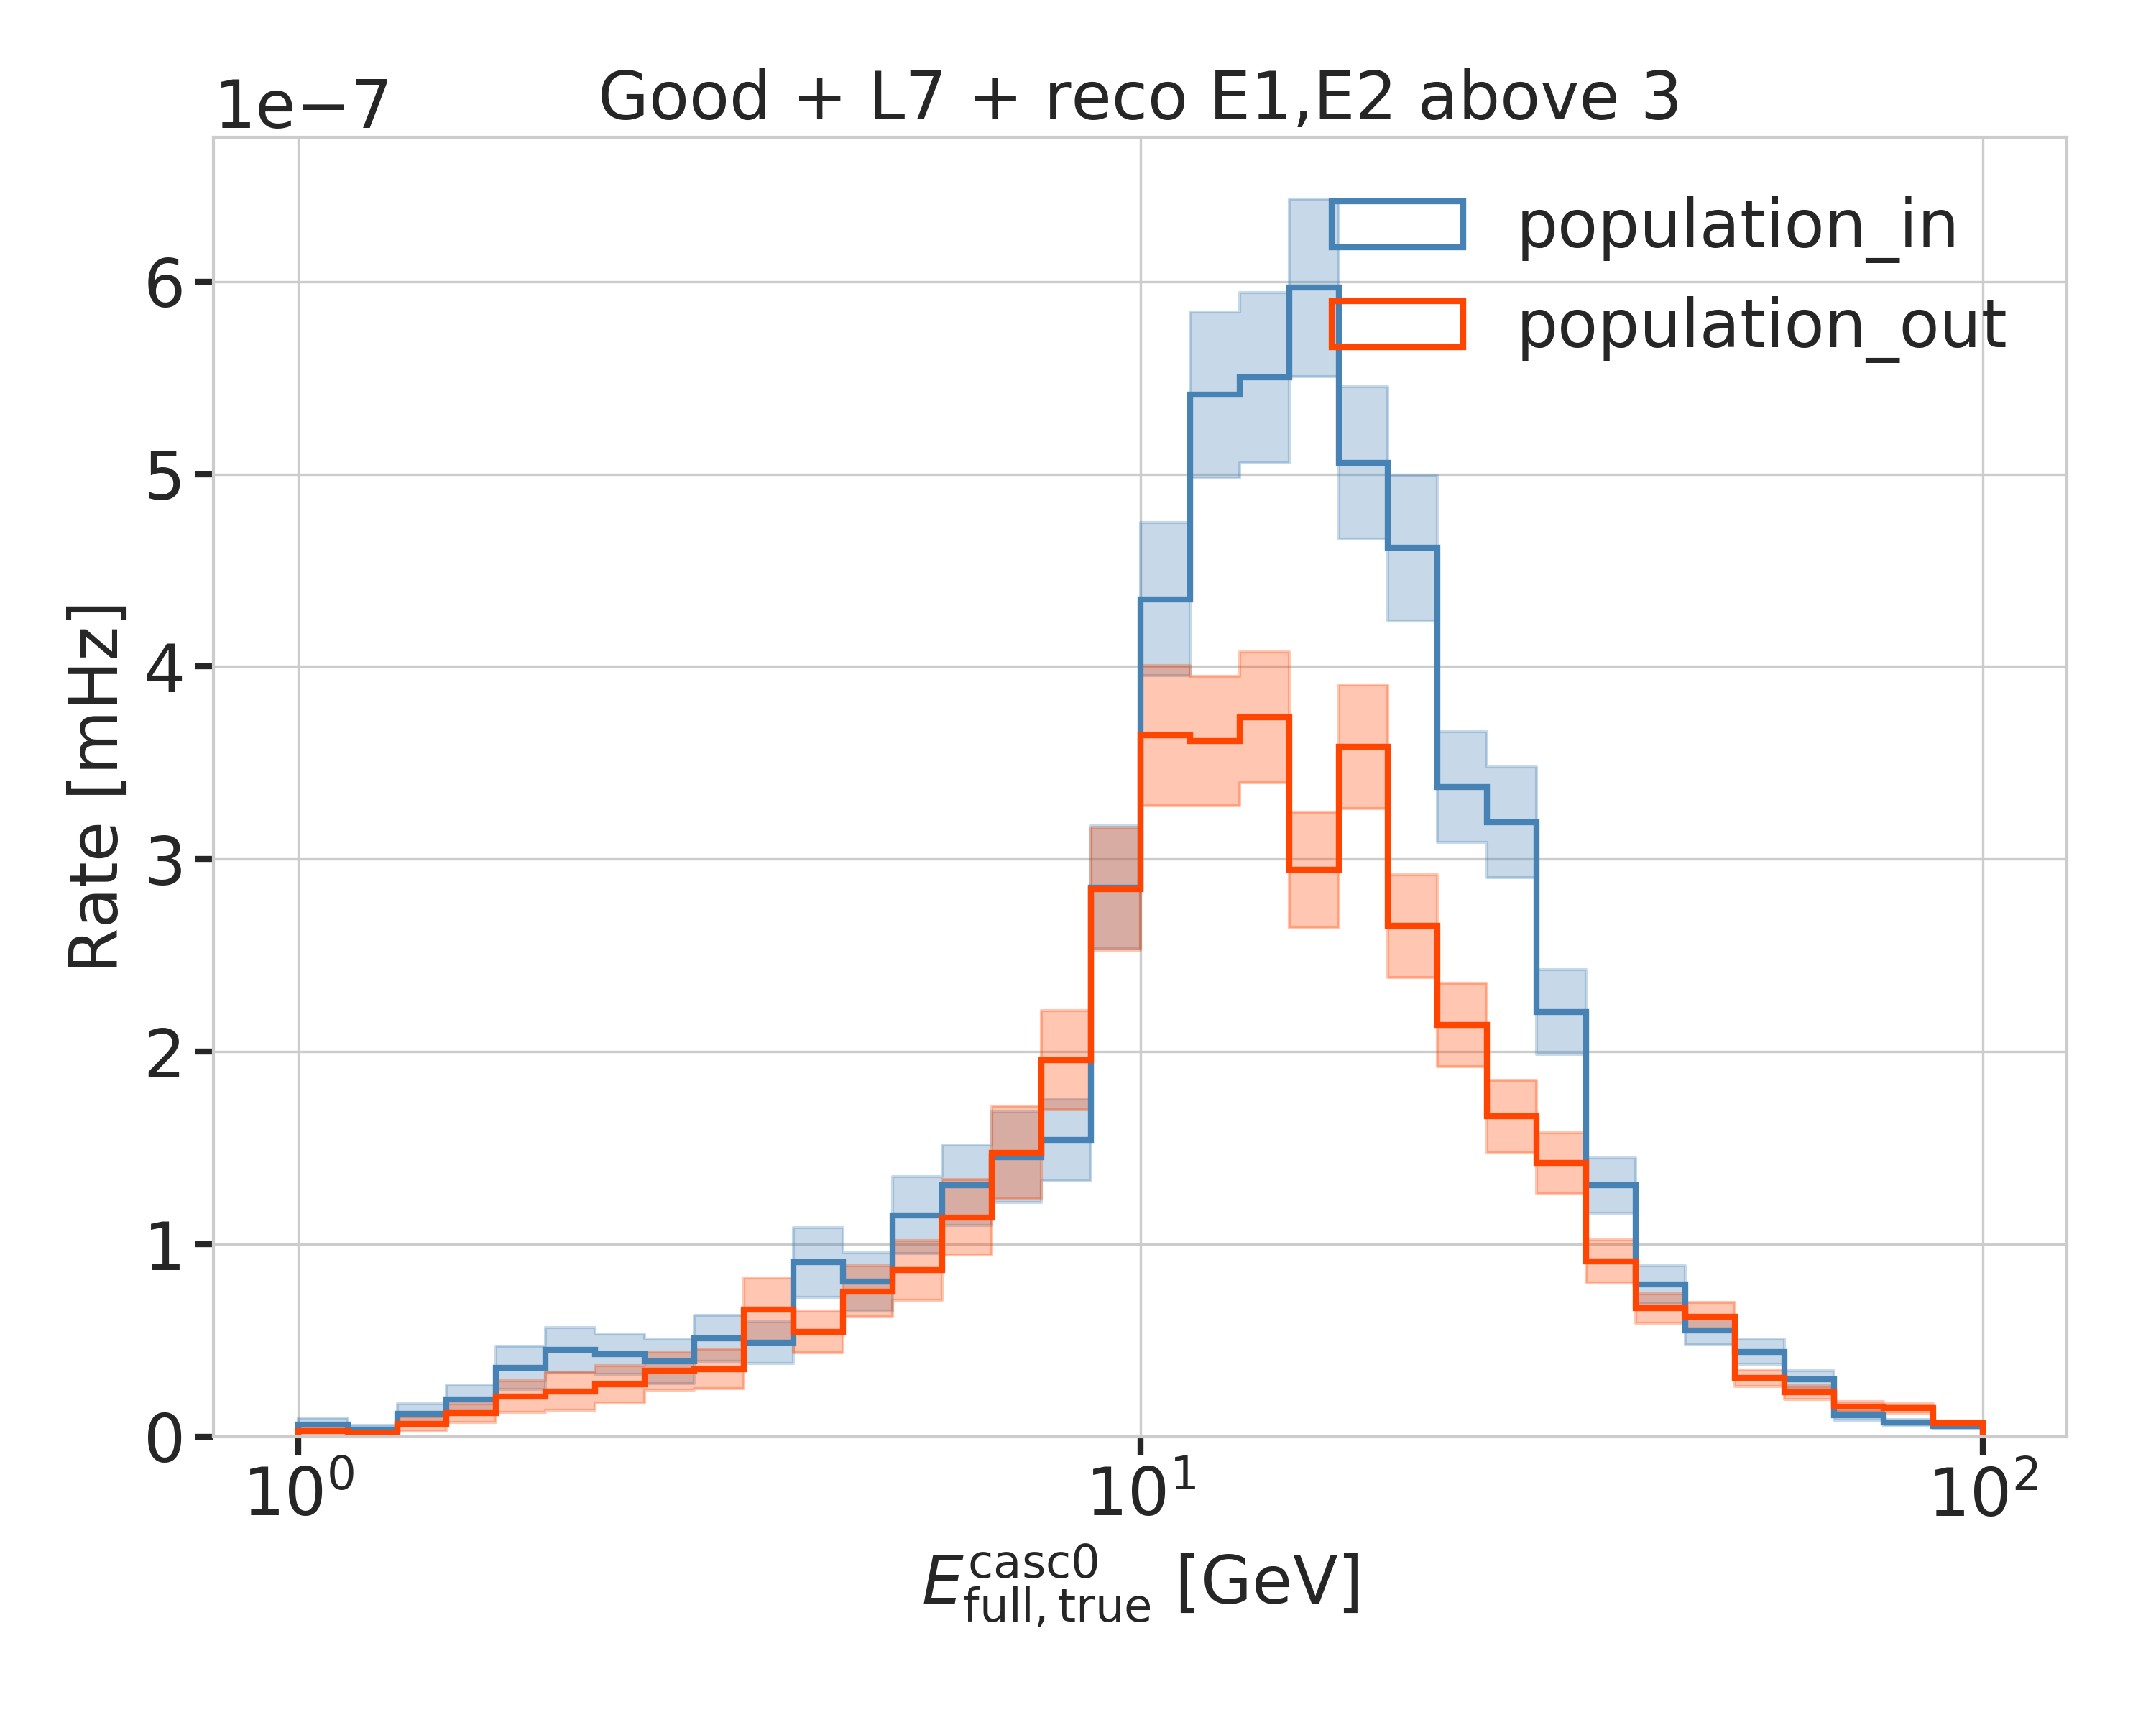
\includegraphics[width=0.49\linewidth]{figures/results/190607/second_population/casc0_energy.png}
    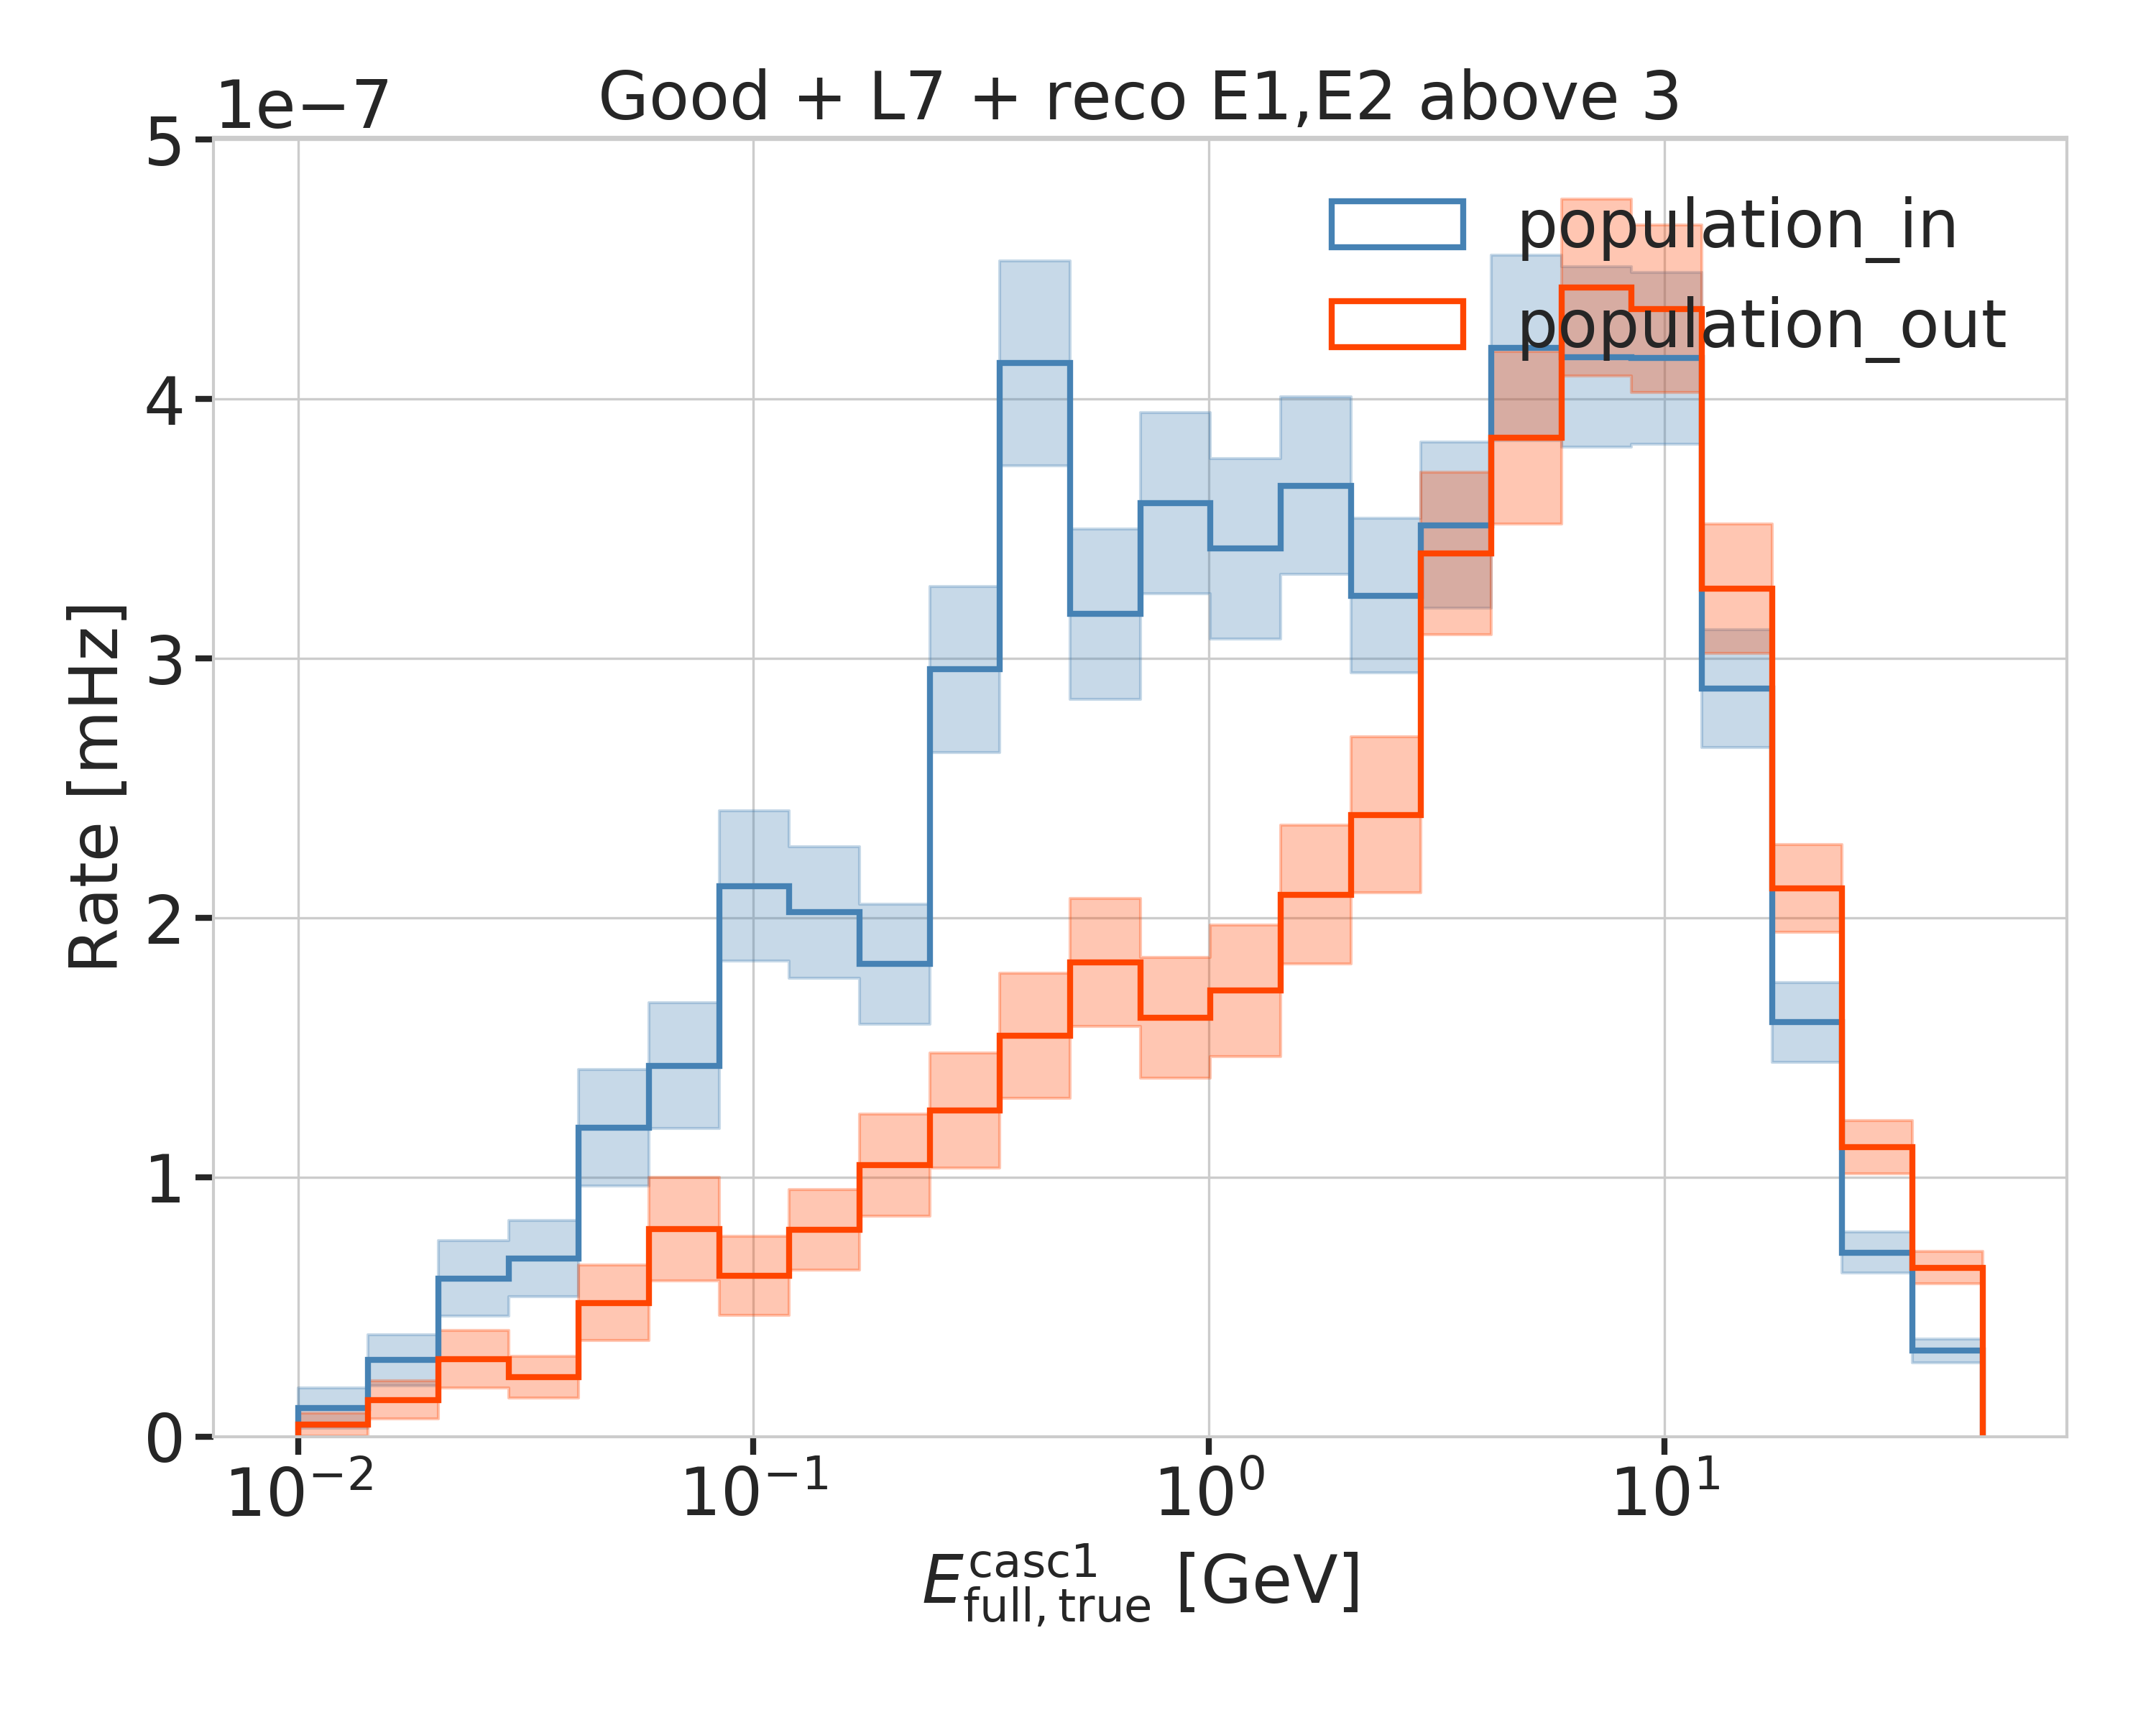
\includegraphics[width=0.49\linewidth]{figures/results/190607/second_population/casc1_energy.png}
    \caption[]{}
    \labfig{population_energy_distributions}
\end{figure*}
\todo{re-make normalized? (ORANGE)}
\todo{fix caption (RED)}

The true energies of both cascades are shown in \reffig{population_energy_distributions}, where it can be observed that the first cascade energy is generally much larger than the second, peaking between \SIrange[range-phrase={~and~}]{10}{20}{\gev}, while the second cascade peaks below \SI{10}{\gev}. For the first cascade there is no significant difference between the two populations, but for the second cascade the badly reconstructed population has a larger fraction of events with lower energies and the distribution is almost uniform in the range of \SIrange{2}{10}{\gev}, while the well reconstructed population has a peak around \SI{10}{\gev} and falls off faster towards lower energies. This is a strong indication that the main reason for the bad reconstruction is the low energy of the second cascade.

% Despite the fact that the split into the two populations was very rudimentary, it is clear that the main reason for the bad reconstruction is the low energy of the second cascade, while other factors, like the position of the second cascade, or the potentially bad input seed direction are also contributing. For a thorough investigation, a more sophisticated separation would be needed, but this is sufficient to conclude that the main reason for the bad reconstruction is the low energy of the second cascade.

% \todo{circle back to the energy distributions I showed somewhere else, and state how the cascade energies are distributed in general (ORANGE)}


\section{Double Cascade Classification}

Even though the performance results show that it is very complicated to reconstruct these low energy double cascade events, the attempt to identify them in the background of SM neutrino events was made. For this purpose a classifier was trained to distinguish between HNL \textit{signal} events and SM neutrino \textit{background} events, using the same preliminary sample of HNL events as was used to assess the reconstruction performance. To mitigate the effect of the bad reconstruction, a set of cuts was applied to make sure the classifier is trained on well reconstructed events. The cuts are a minimum reconstructed energy of both cascades of \SI{5}{\gev} and a minimum reconstructed decay length of \SI{40}{\meter}. and they are applied to both signal and background events.

\begin{figure}[h]
    \centering
    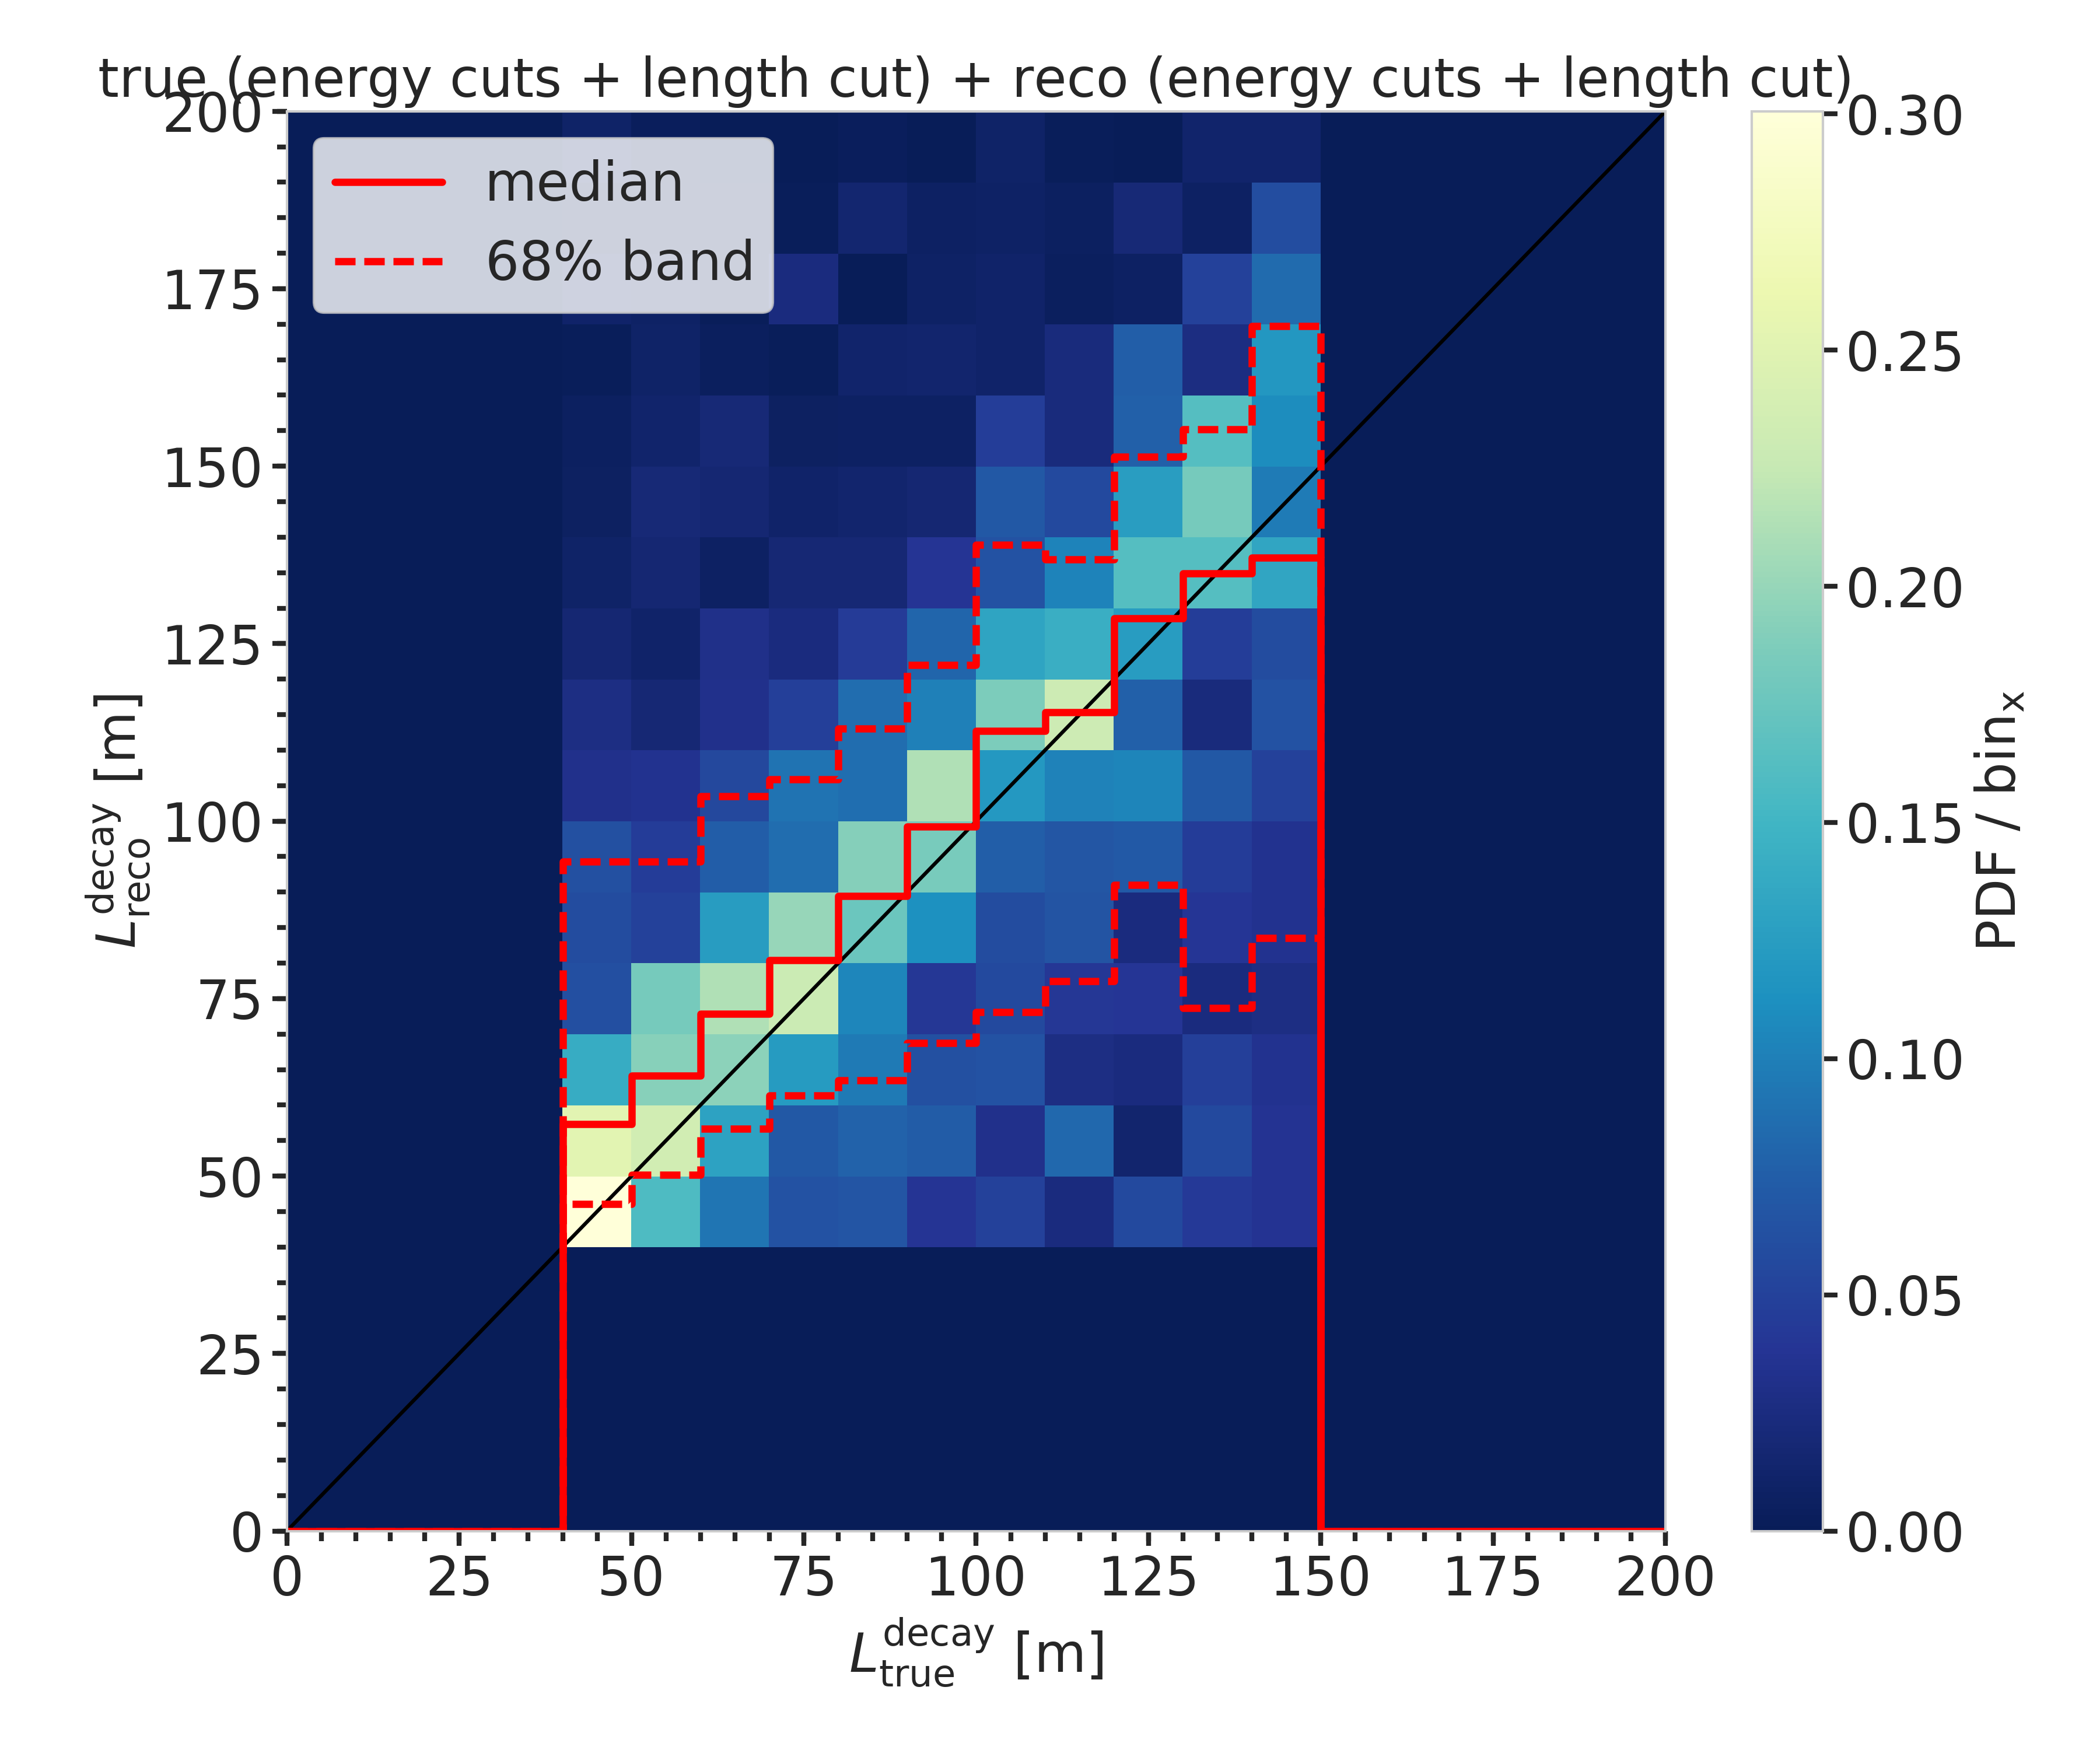
\includegraphics{figures/results/190607/classification/reco_decayL_vs_true_decayL_reco_energy_cut_and_reco_length_cut_and_true_energy_cut_and_true_length_cut_step_contours_weighted.png}
    \caption[]{}
    \labfig{classifier_cuts_length_2d_hist}
\end{figure}
\todo{fix caption (RED)}

Additionally, some cuts on the true energies and decay length were applied for the signal, which are a minimum true energy of both cascades of \SI{5}{\gev}, and a true decay length between \SIrange[range-phrase={~and~}]{40}{150}{\meter}. These were chosen to make sure the HNL events were theoretically double cascade like and at a sensible length scale inside DeepCore. \reffig{classifier_cuts_length_2d_hist} shows the decay length two-dimensional histogram after the cuts were applied.

The classifier used was a \textit{Boosted Decision Tree (BDT)} from the \textit{\textsc{scikit-learn} (sklearn)} package \sidecite{sklearn} and the input features are taken from the double cascade reconstruction explained in \refsec{dc_reconstruction} as well as some additional variables from earlier levels of the processing explained in \refsec{processing_chain}. \reffig{example_BDT_features} shows the distributions of two example input features, where the left plot shows the output probability of the classifier trained to distinguish track from cascade like events, which is used in the oscillation analysis, and the right plot shows the reconstructed decay length from the double cascade reconstruction. Shown are the distributions for the the HNL signal, the individual background components, and the total background. 

\begin{figure*}[h]
	\centering
    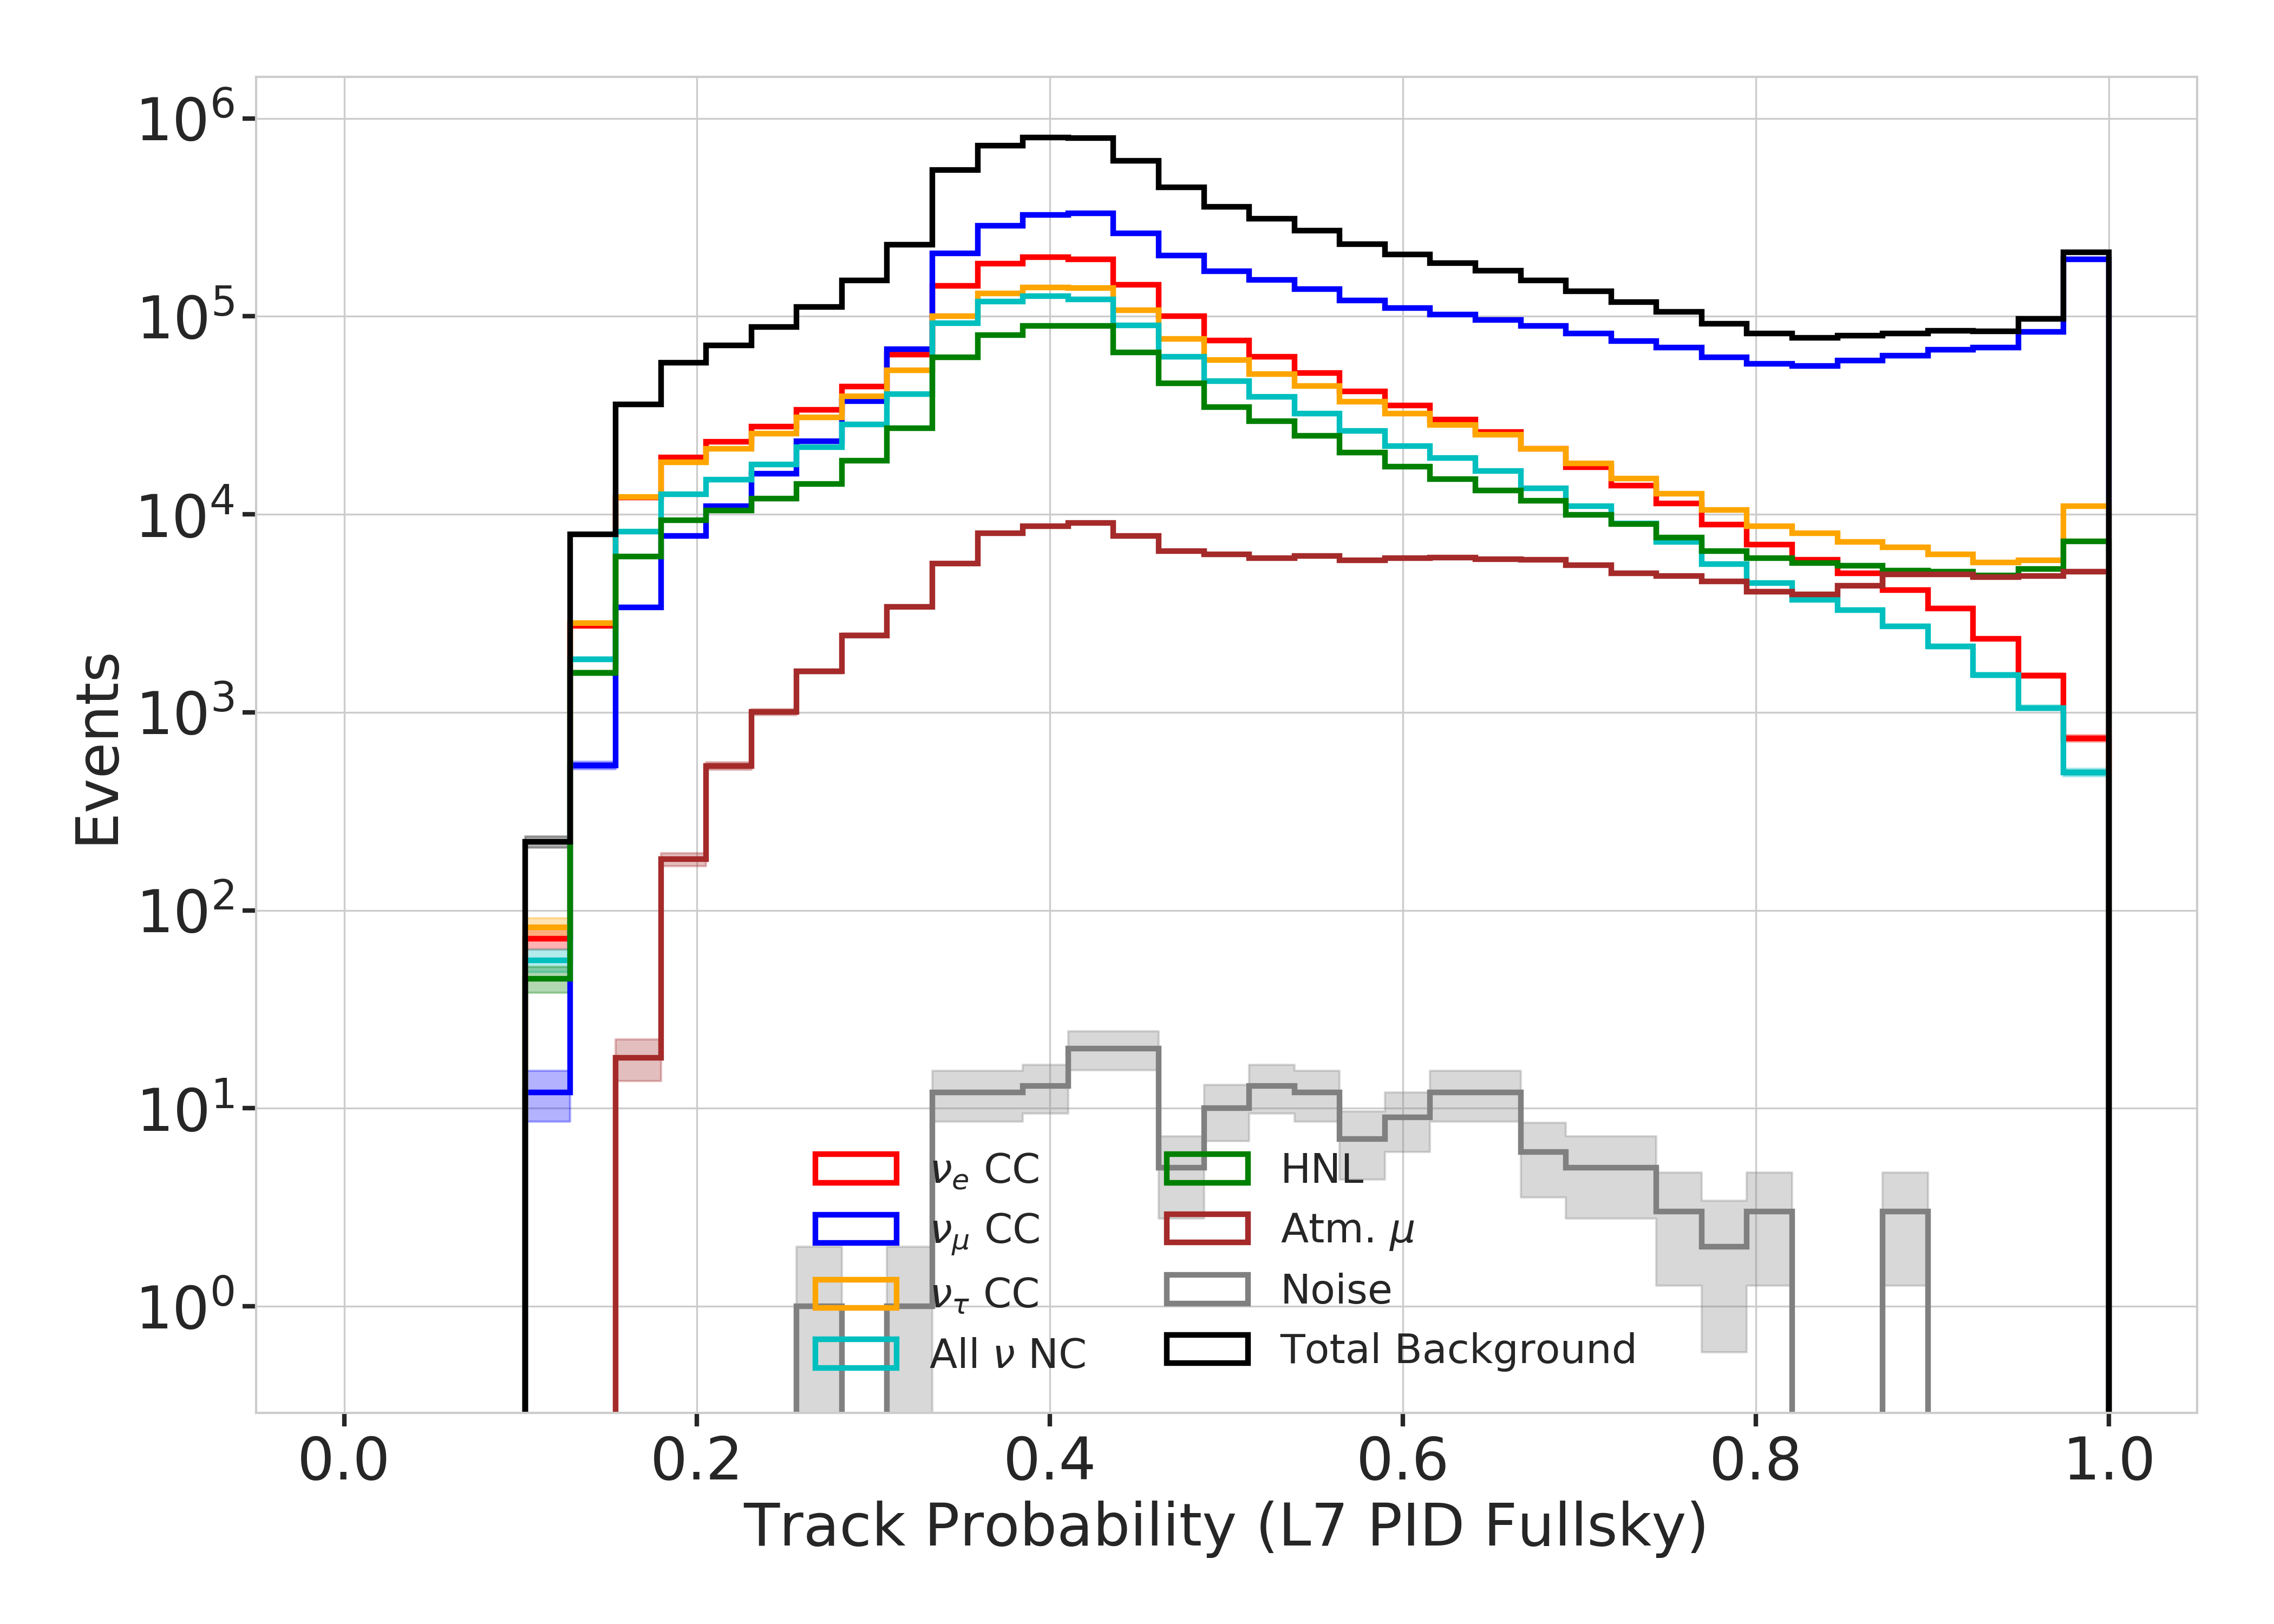
\includegraphics[width=0.49\linewidth]{figures/results/190607/classification/1_d_distr_L7_PIDClassifier_FullSky_ProbTrack_with_ratio_unweighted.png}
    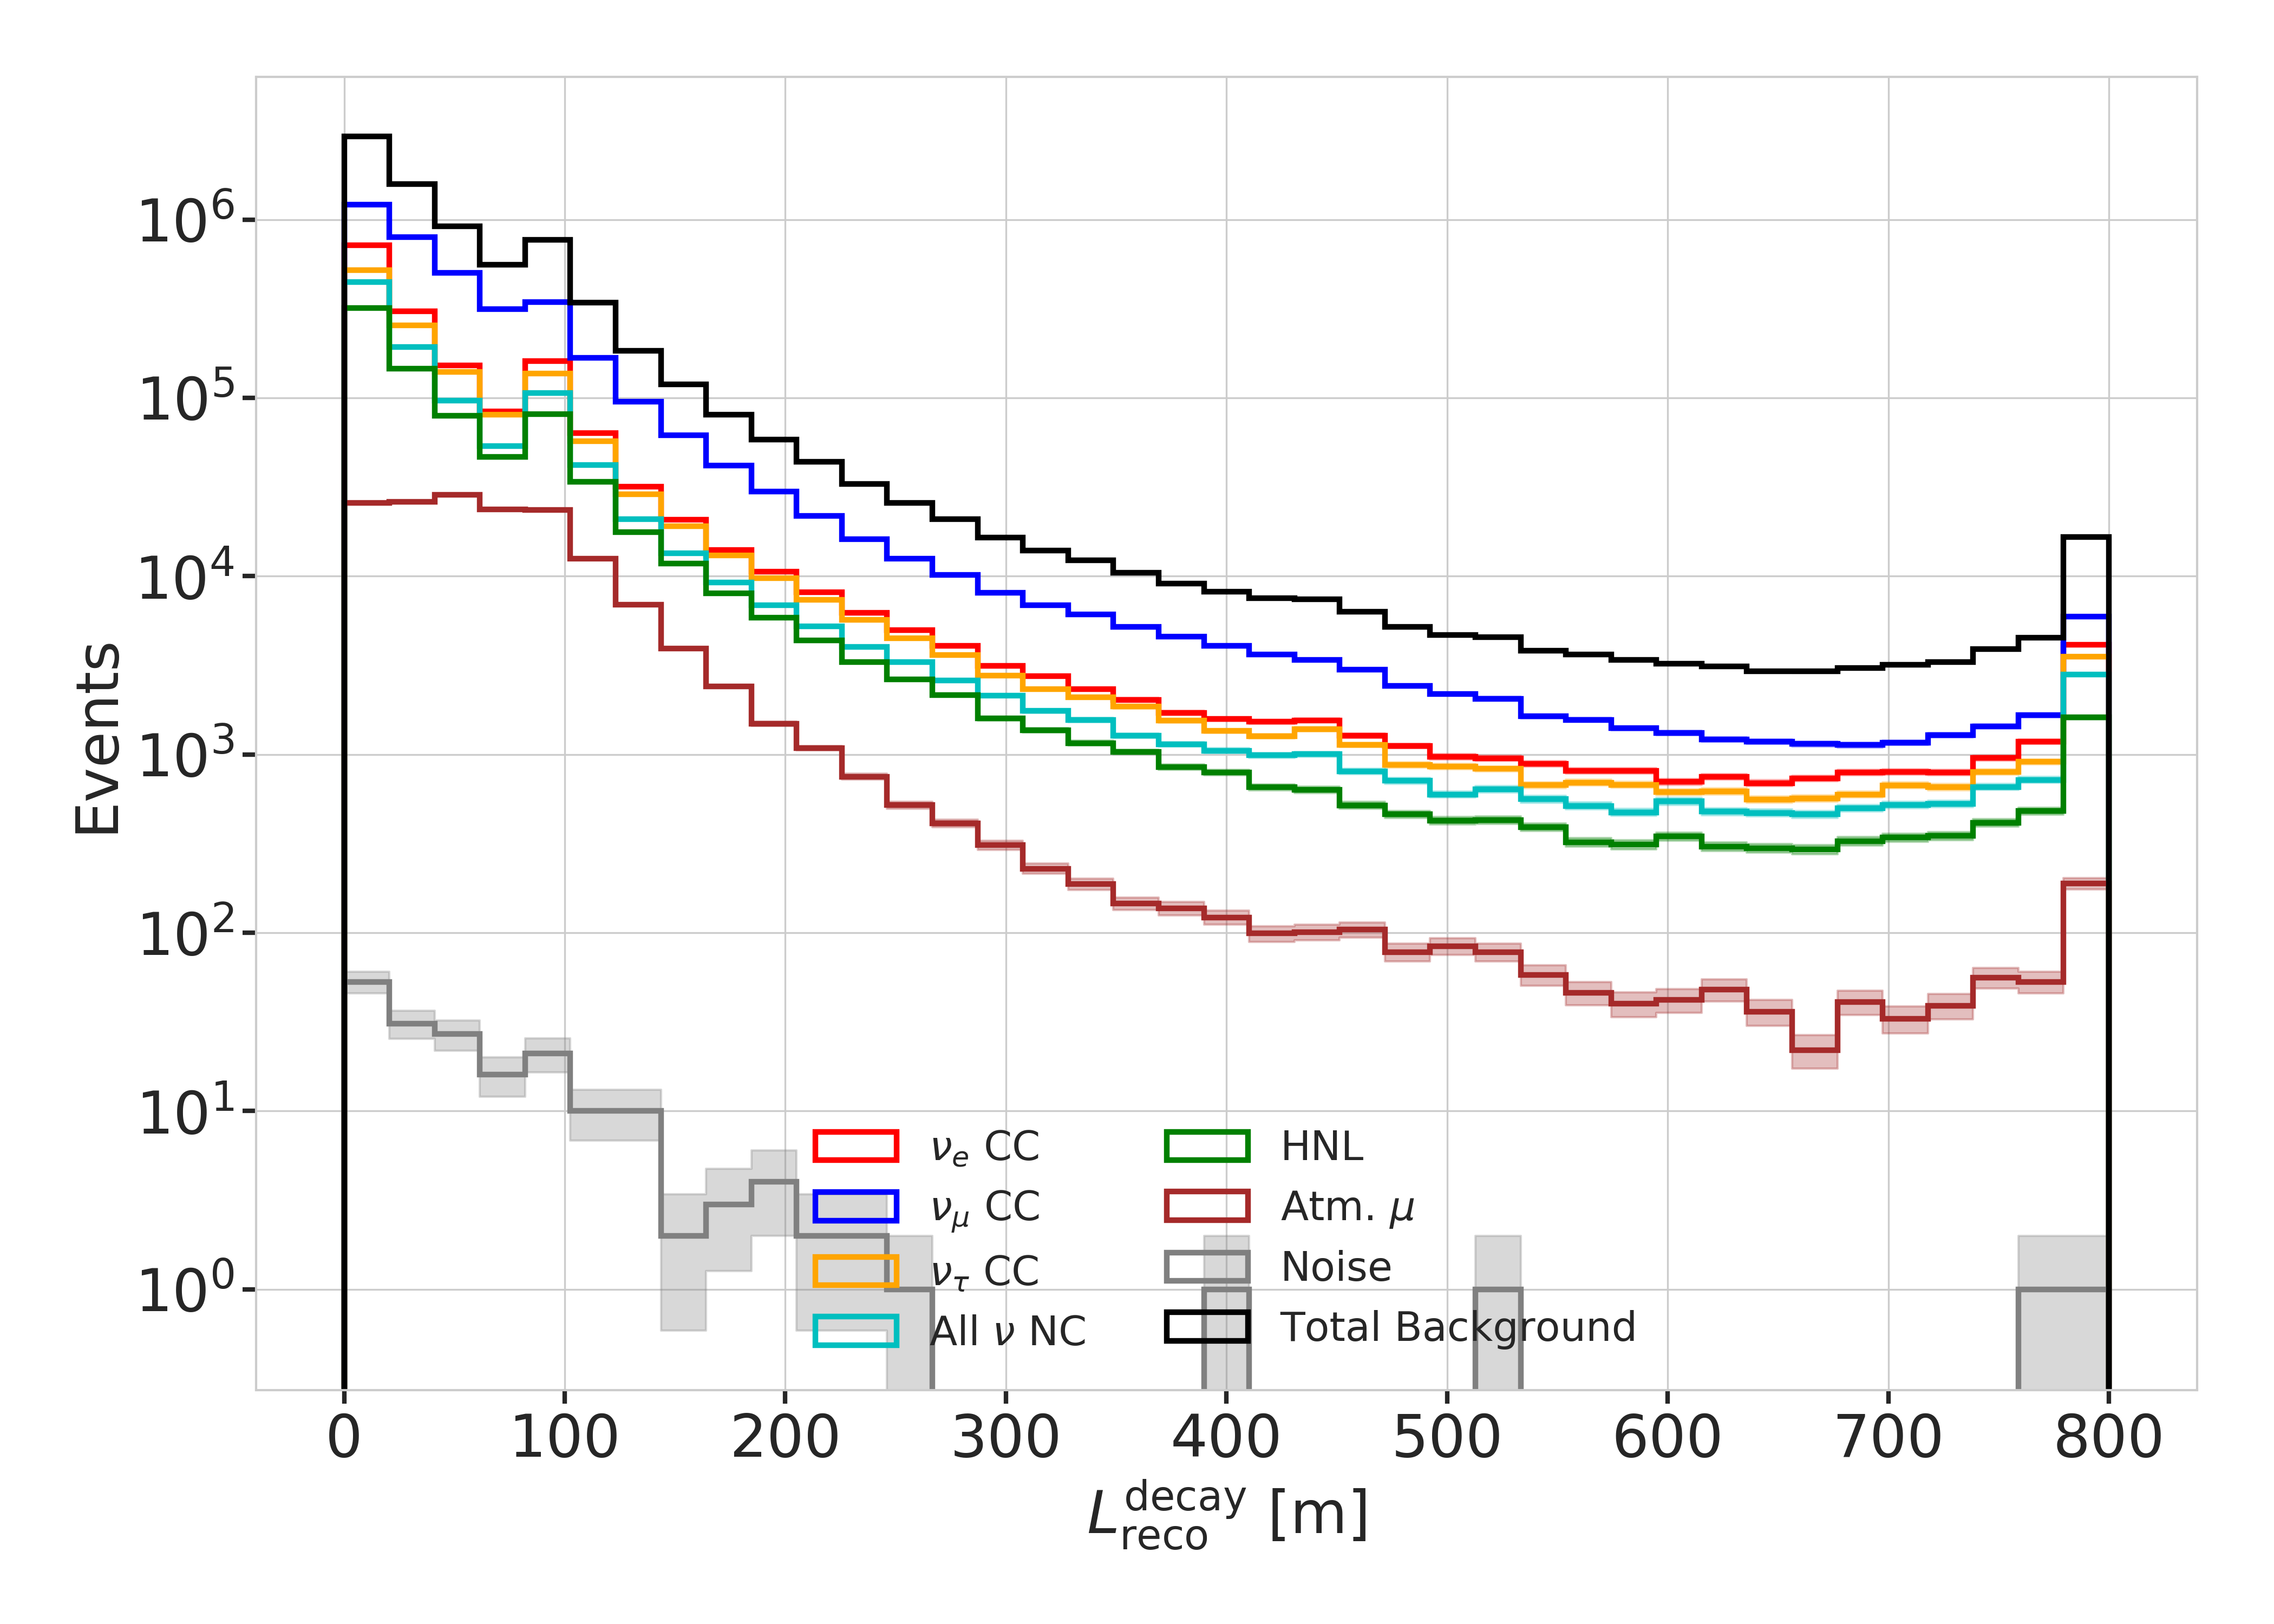
\includegraphics[width=0.49\linewidth]{figures/results/190607/classification/1_d_distr_reco_decayL_with_ratio_unweighted.png}
    \caption[]{}
    \labfig{example_BDT_features}
\end{figure*}
\todo{fix caption of this figure (RED)}

A single classifier and a combination of two classifiers were tested. The single classifier was trained to distinguish between HNL signal events and all SM background events at once. The two classifiers were trained separately, one to distinguish signal from track like background, and the other to distinguish signal from cascade like background. Since the SM neutrino events at these energies are either track like or cascade like, the latter approach was expected to perform better. Despite the fact that several combinations of features and classifier hyperparameters were tested, it was not possible to identify a pure double cascade region with a single classifier.

% \reffig{example_classifier_probability} shows the output probability of the classifier trained to distinguish double cascades from tracks, applied to the full data sample containing all signal and background events. A probability of 1 means very signal like, where only the region close to 1 is shown to highlight that there is always signal and background events in every bin.

% \begin{figure}[h]
%     \centering
%     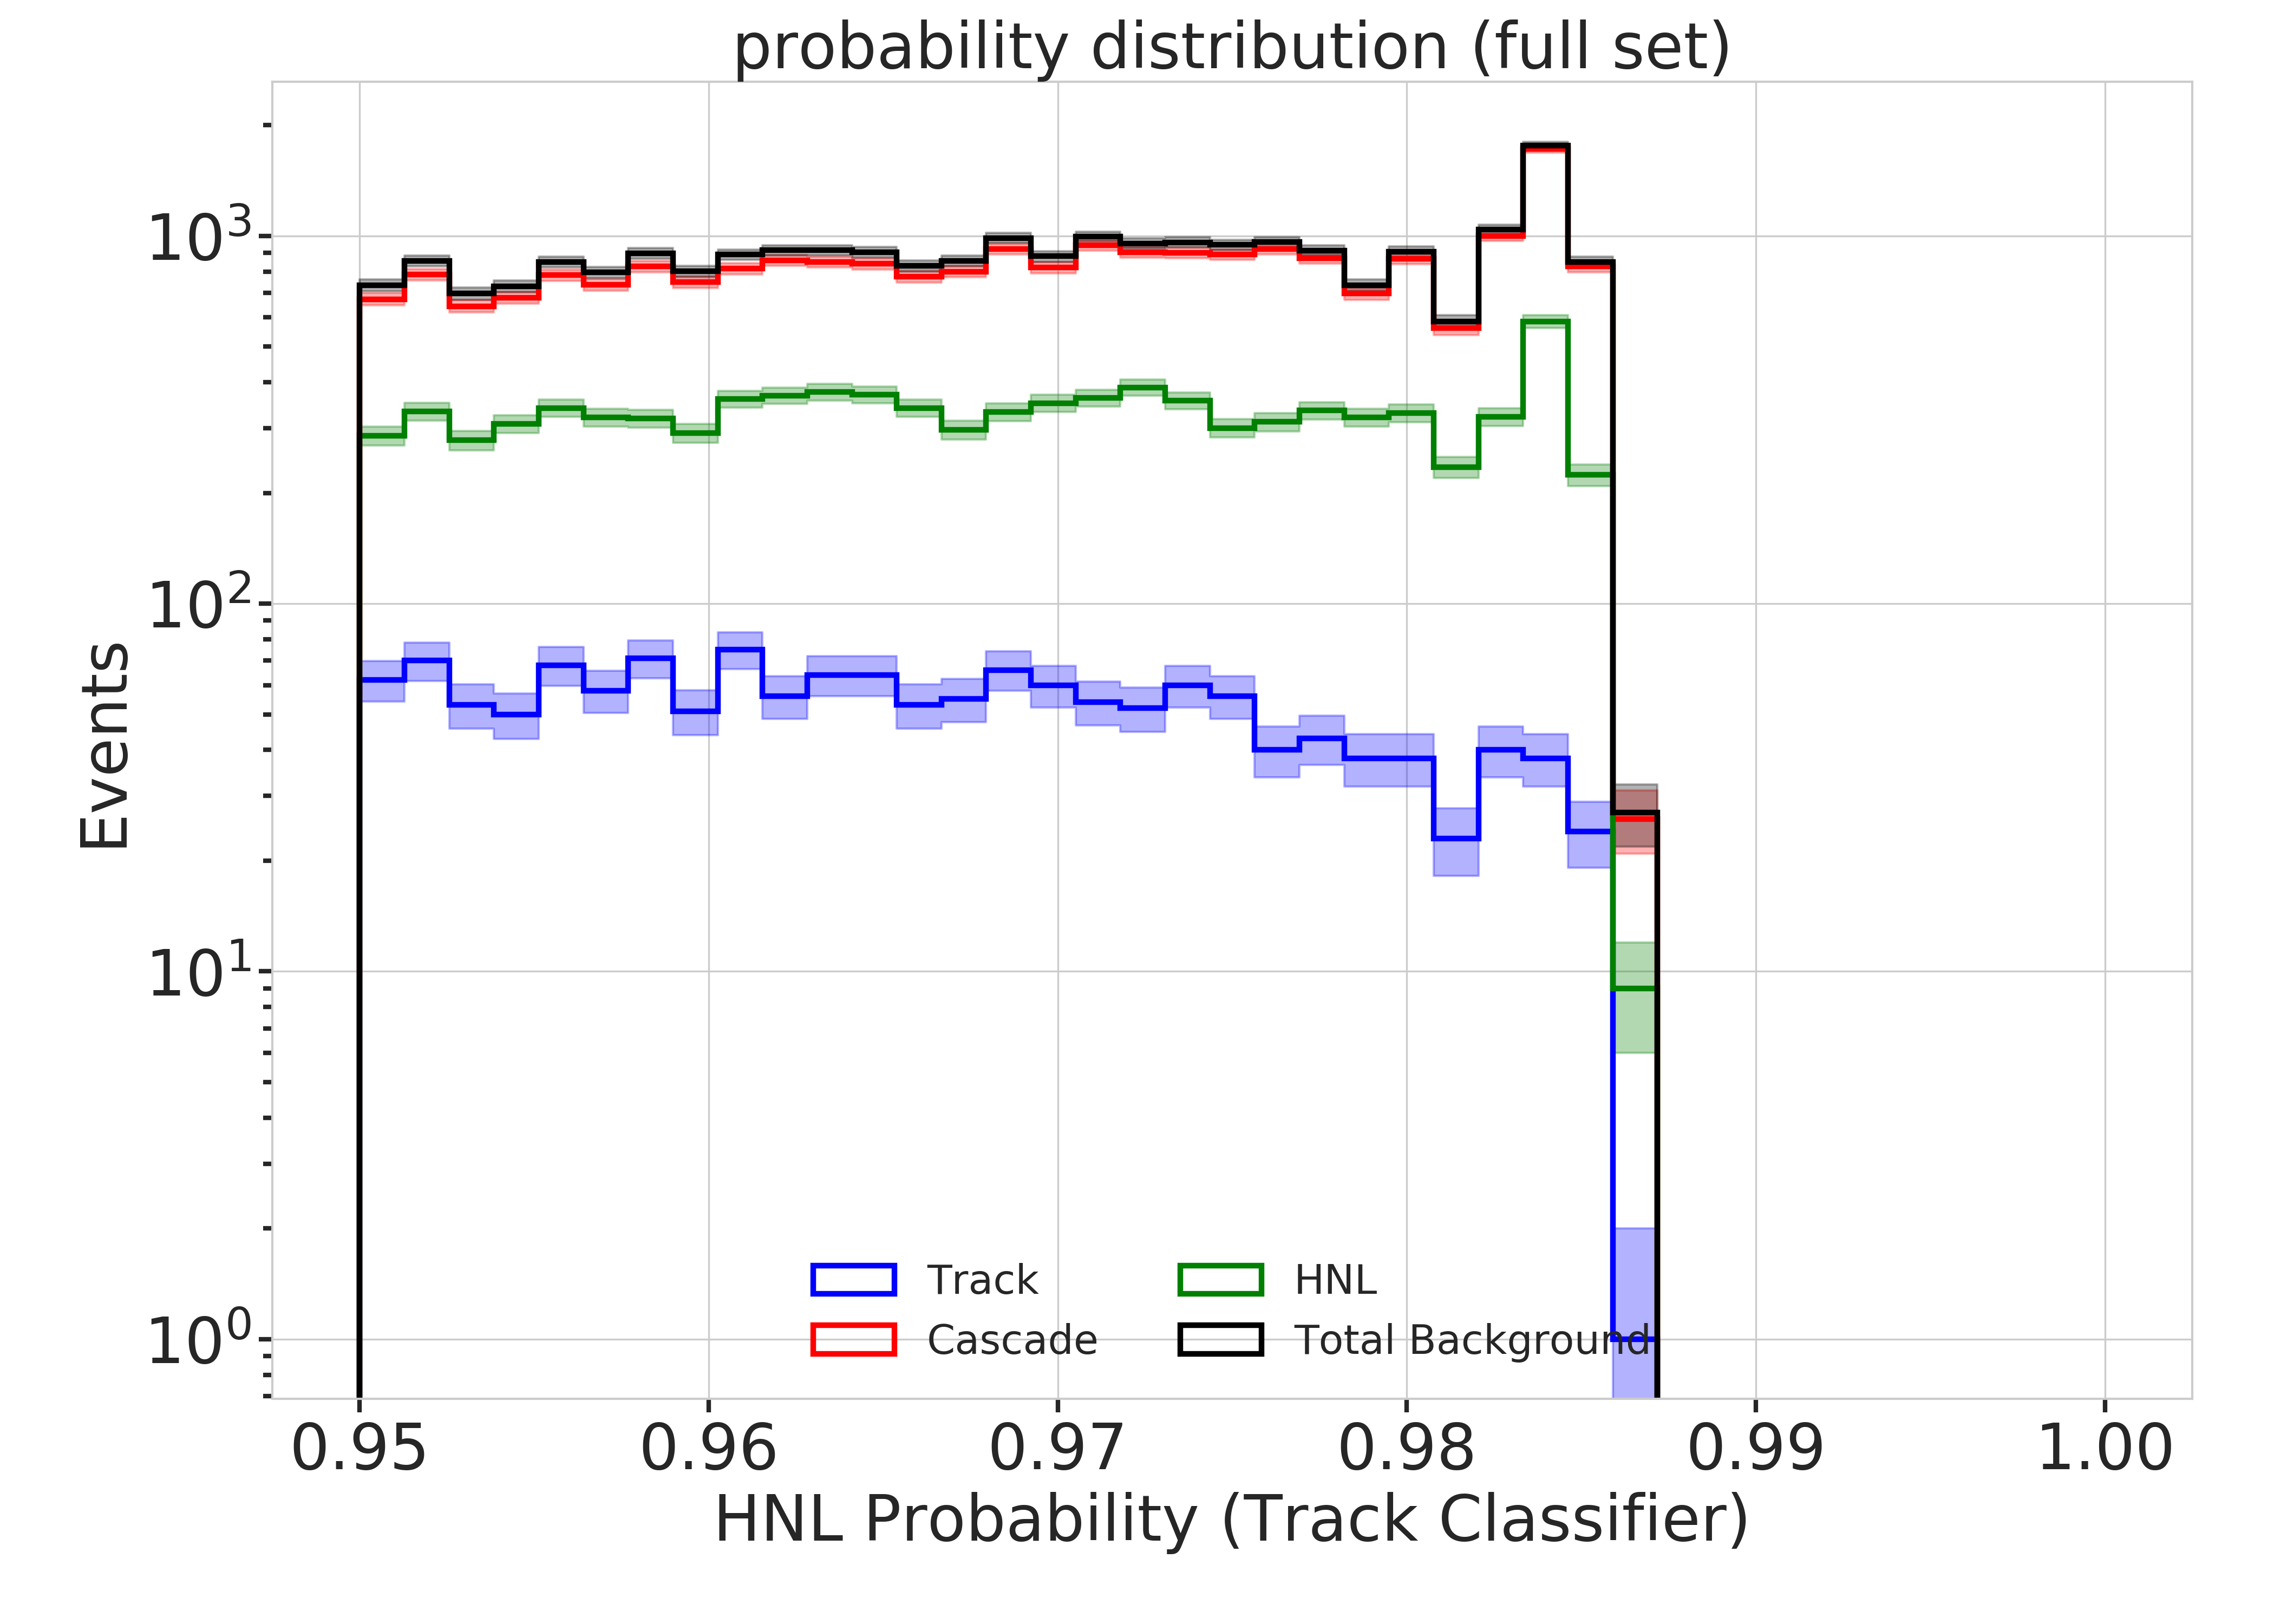
\includegraphics{figures/results/190607/classification/1_d_distr_hnl_prob_track_classifier_full_stats_unweighted.png}
%     \caption[]{}
%     \labfig{example_classifier_probability}
% \end{figure}
% \todo{fix caption (RED)}

By applying the two classifiers trained to distinguish signal from track and signal from cascade, it is possible to select a region with only signal events. This is visualized in \reffig{two_classifier_selection}\todo{Make a single plot, showing S/B or so? (RED)}, where the probabilities of 1 implies very signal like, and only the regions close to 1 are shown for both outputs, to highlight the interesting region, where a pure HNL sub-sample can be selected. When physical weights are applied to those signal events however, the expected event rate is very low, and even by assuming a highly optimistic mixing of 1, it would take more than \SI{20}{years} of data taking to observe a single event. Additionally, with this low simulation statistics the prediction is not very reliable, either. Making a weaker cut to select a signal like region will contain a large amount of background events, which dominate over the signal at $\sim2$ orders of magnitude for a mixing of $0.1$. The conclusion from this is, that with the current selection and reconstruction chain and a classical BDT, it is not possible to distinguish signal events at a level feasible to perform an analysis.

\begin{figure*}[h]
	\centering
    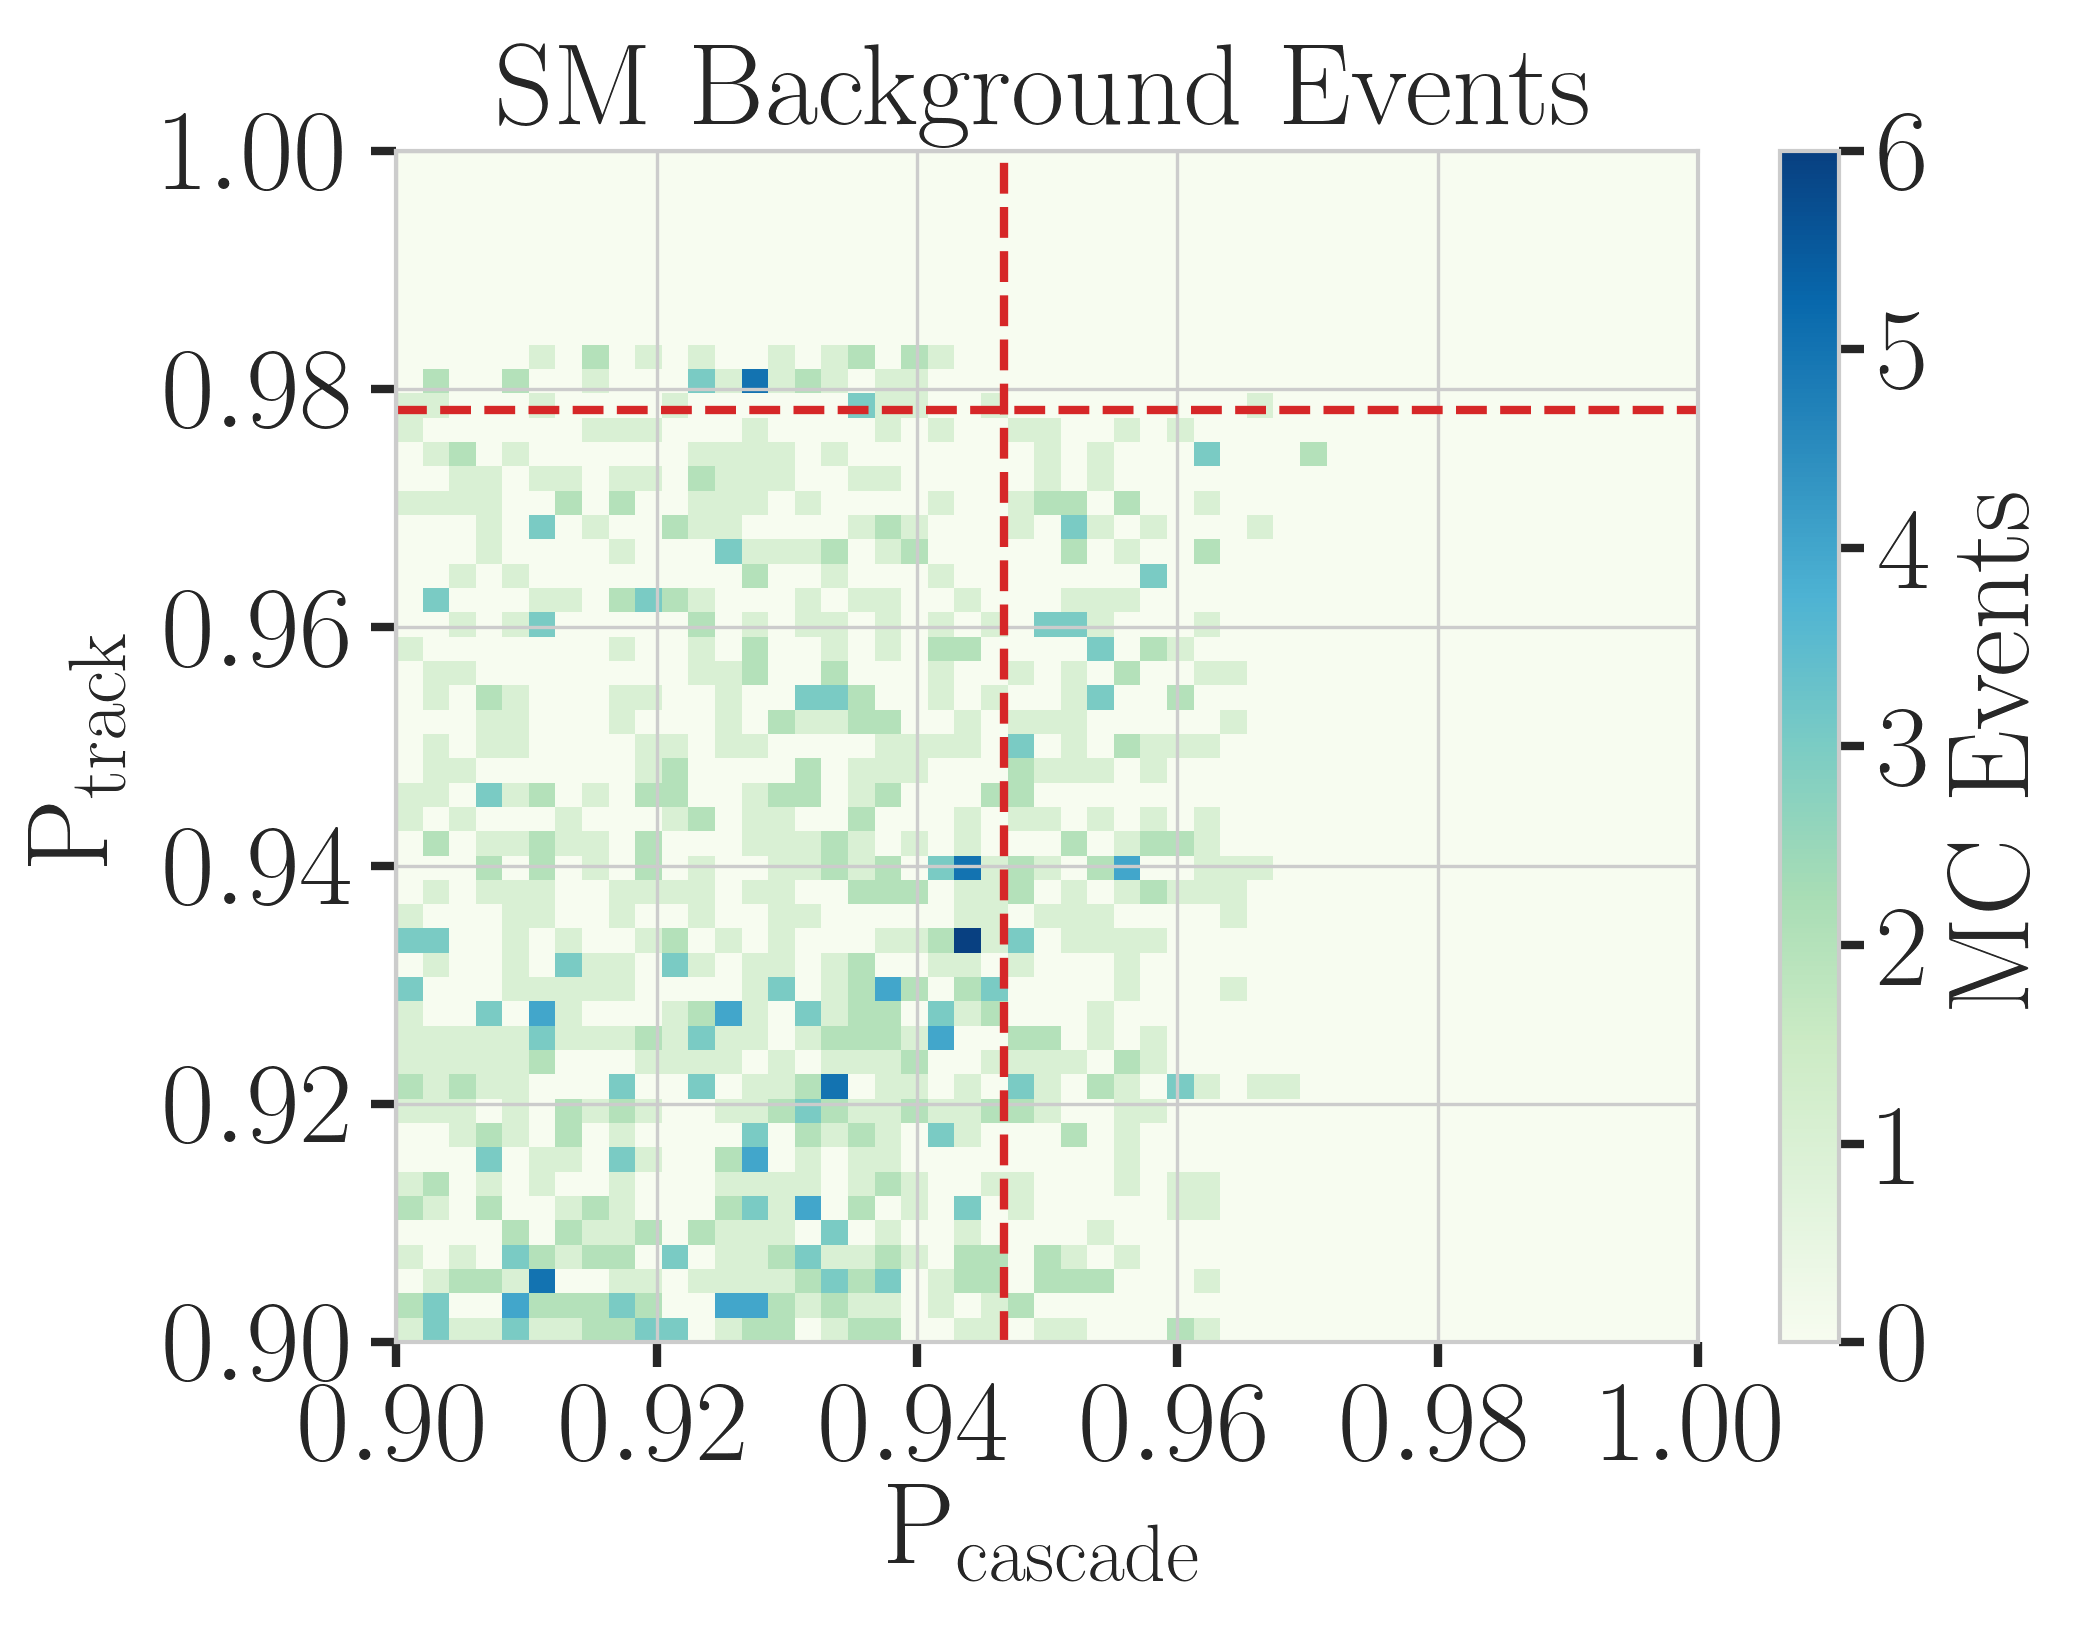
\includegraphics[width=0.49\linewidth]{figures/results/190607/classification/cascade_vs_track_class_prob_background_full_stats.png}
    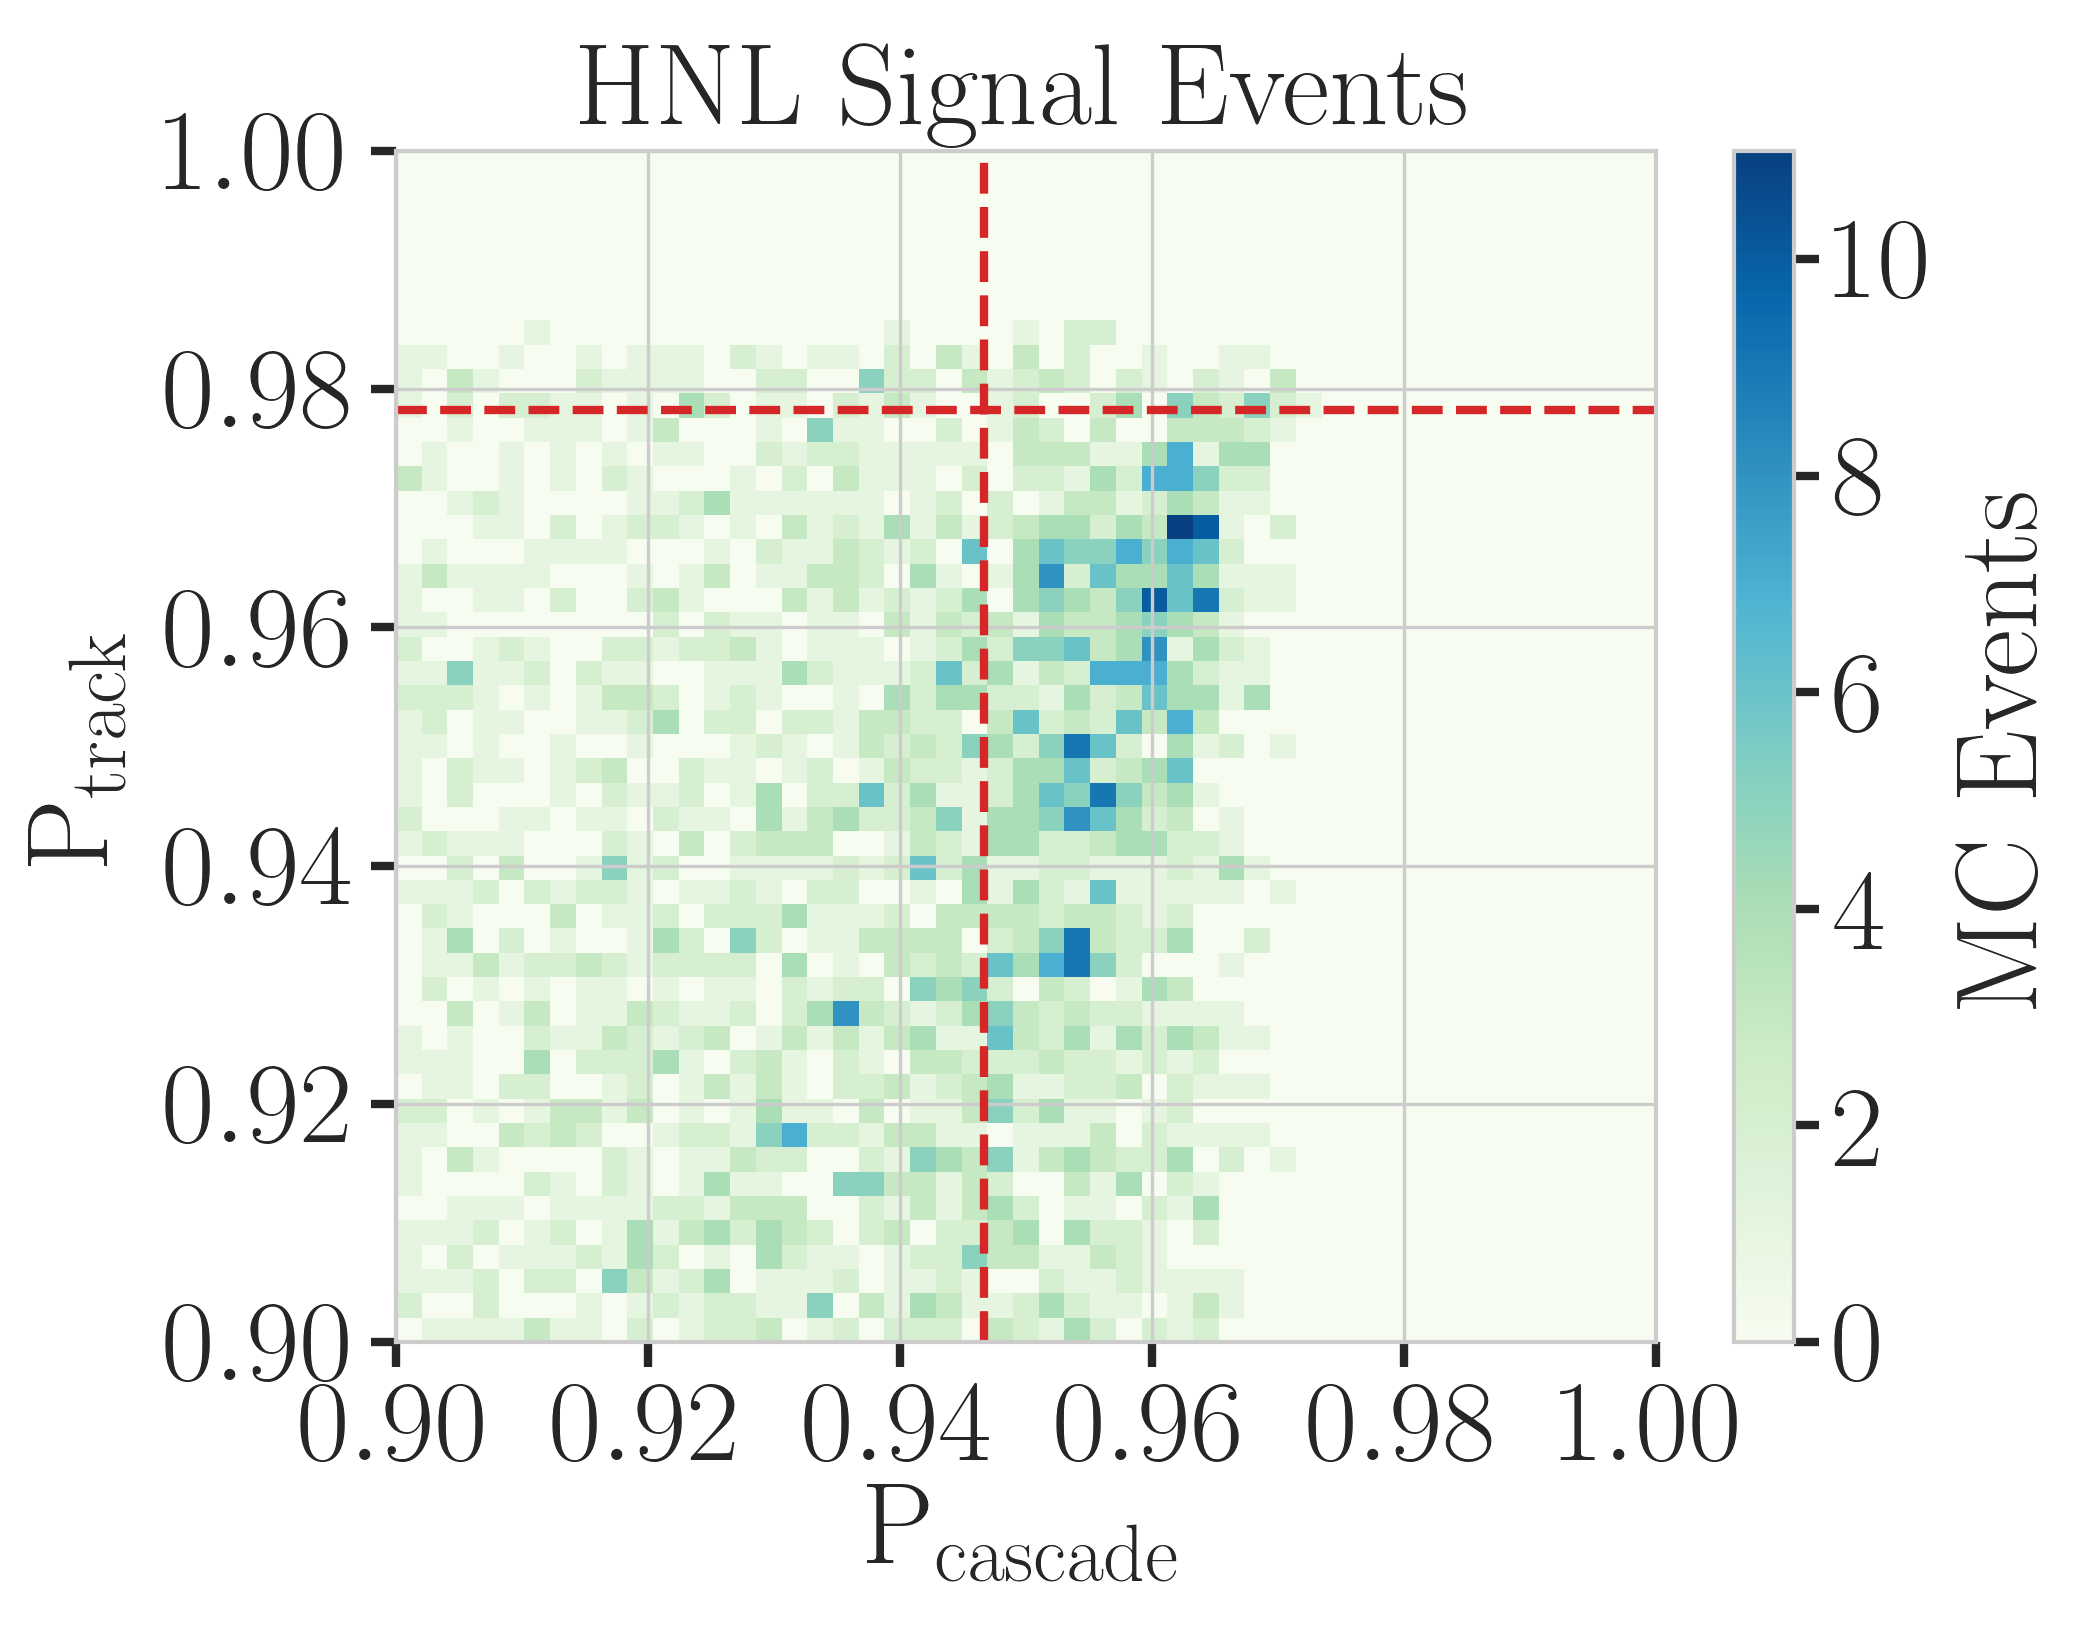
\includegraphics[width=0.49\linewidth]{figures/results/190607/classification/cascade_vs_track_class_prob_hnl_full_stats.png}
    \caption[]{}
    \labfig{two_classifier_selection}
\end{figure*}
\todo{fix caption of this figure (RED)}


\section{Generalized Double Cascade Performance}

All the above results were obtained using preliminary development versions of the model dependent HNL simulation. To investigate the effect of the low energy event selection and the double cascade reconstruction performance in a more generic way, the model independent simulation introduced in \refsec{model_independent_simulation} is used to repeat the performance checks and to run a series of additional checks. The important advantage of the model independent samples is the controllable parameter space, especially in cascade energies and decay length, because the event kinematics are not coupled to the underlying HNL model, but can be chosen freely. This means that some benchmark edge cases can be investigated, and the performance can also be assessed for a realistic scenario in addition to mapping out the effects of the event selection and where the reconstruction breaks down.


\subsection{Idealistic Events}

\begin{marginfigure}
    \centering
    % [trim=left bottom right top, clip]
    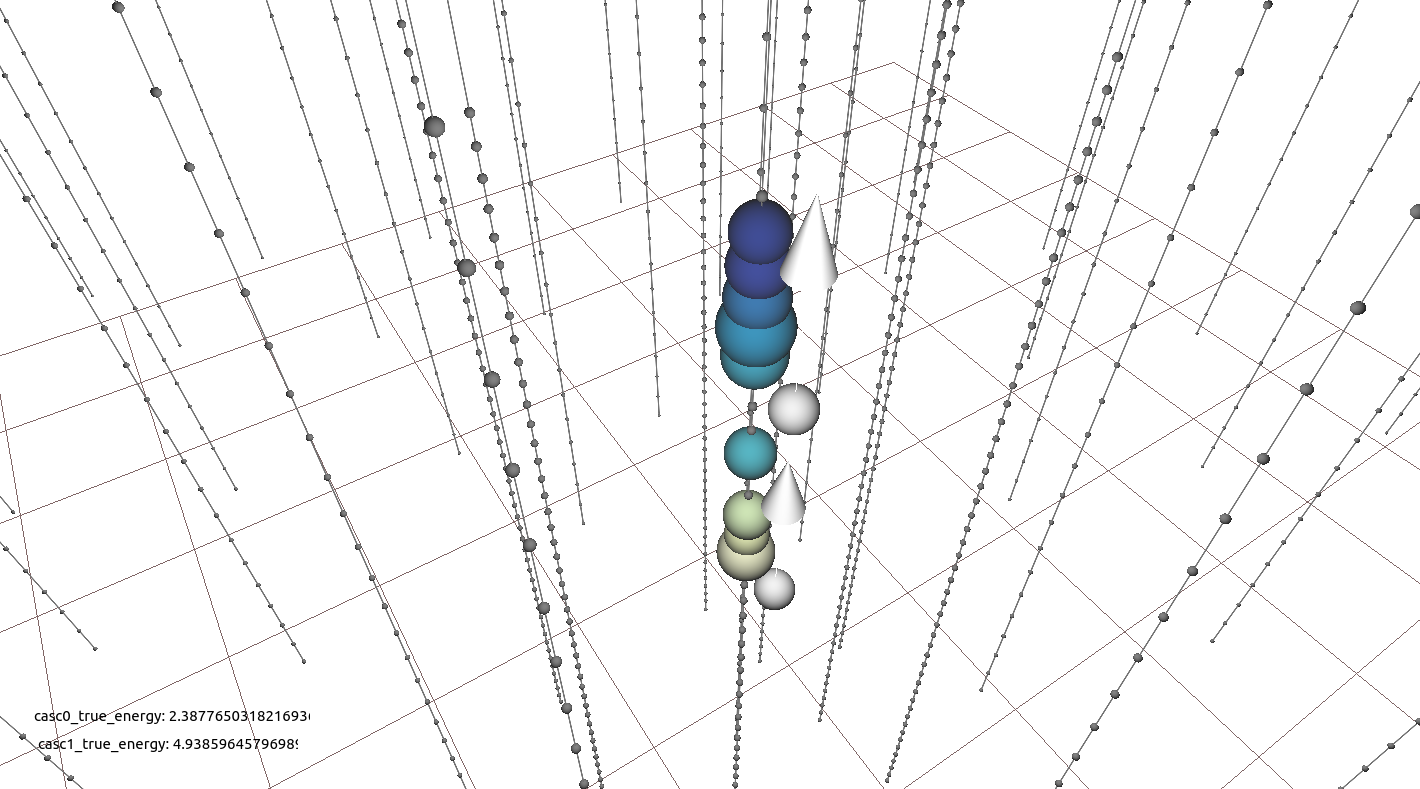
\includegraphics[trim=270 40 225 35, clip]{figures/model_independent_simulation/upgoing_e0_2.4_e1_4.9_v2.png}
    \caption[Event view of an idealistic double cascade event]{Event view of an idealistic double cascade event, with cascade energies of \SI{2.4}{\gev} and \SI{4.9}{\gev}, and a decay length of \SI{65.8}{\meter}. The colored spheres show the DOMs that have observed light, where the size is proportional to the number of observed photons and the color indicates the time (yellow is early, blue is late). The strings are shown as black lines, with small spheres indicating the DOM positions, and the true cascade vertices and directions are shown as white spheres with white arrows.}
    \labfig{up-going_example_event}
\end{marginfigure}

The \textit{best case} scenario to observe an event is to be directly on top of a string with a straight up-going direction. Using the simulation sample introduced in \refsec{simplistic_samples} and running the double cascade reconstruction from \refsec{dc_reconstruction} on these events, it is possible to estimate the performance limit of the reconstruction. \reffig{up-going_example_event} shows one example event view from that sample, where the cascade energies are \SI{2.4}{\gev} and \SI{4.9}{\gev}, and the decay length is \SI{144.5}{\meter}. It can be seen that despite the low energies, both cascades deposit light in the DOMs and the reconstruction is expected to work.

The performance of the length reconstruction is shown in \reffig{idealistic_length_resolutions}, where the median of the absolute, fractional decay length resolution is shown on the left and the two-dimensional histogram of the reconstructed versus the true decay length is shown on the right. For these results and the following, all events that were reconstructed with non-zero cascade energies and non-zero decay length are used, and the events are unweighted. The length is very well reconstructed, with the median resolution being below \SI{30}{\percent} above a true decay length of $\sim$\SI{10}{\meter}, and falling off with increasing true length, down to $\sim$\SI{10}{\percent} at \SI{100}{\meter}.

\begin{figure*}[h]
	\centering
    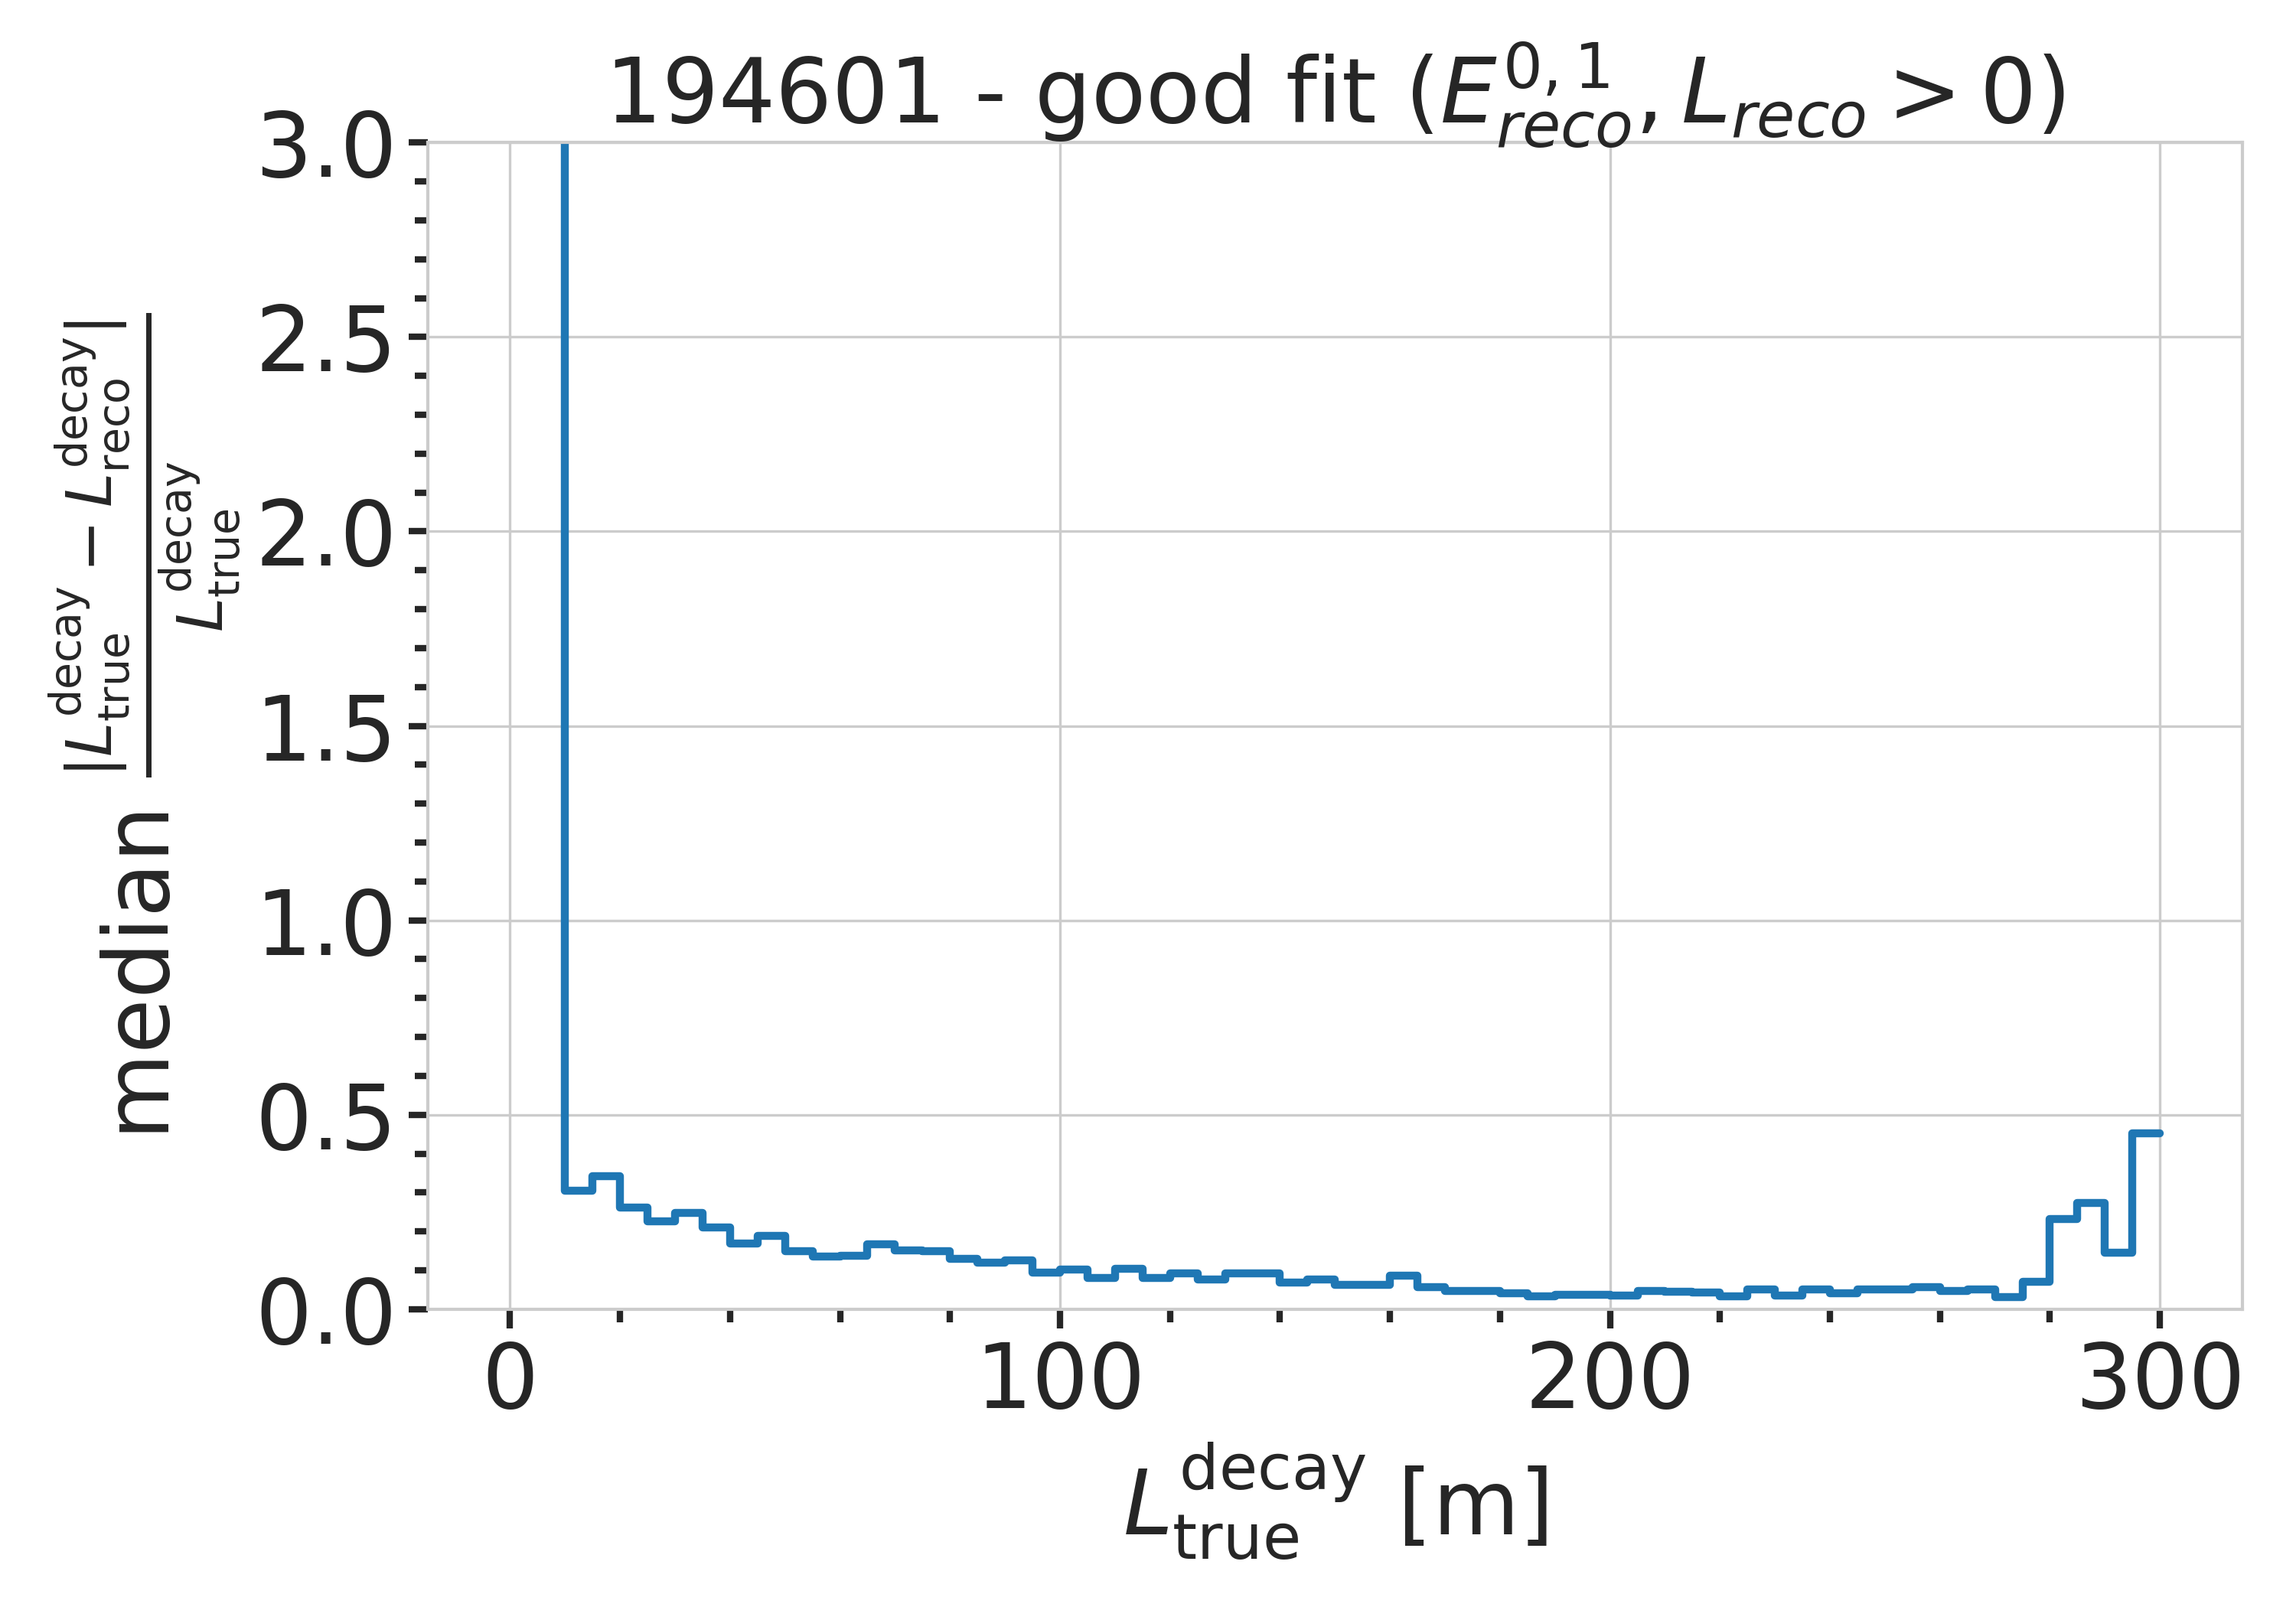
\includegraphics[width=0.49\linewidth]{figures/model_independent_simulation/results/idealistic/194601_median_decay_length_resolution_goodfit_log_unweighted.png}
    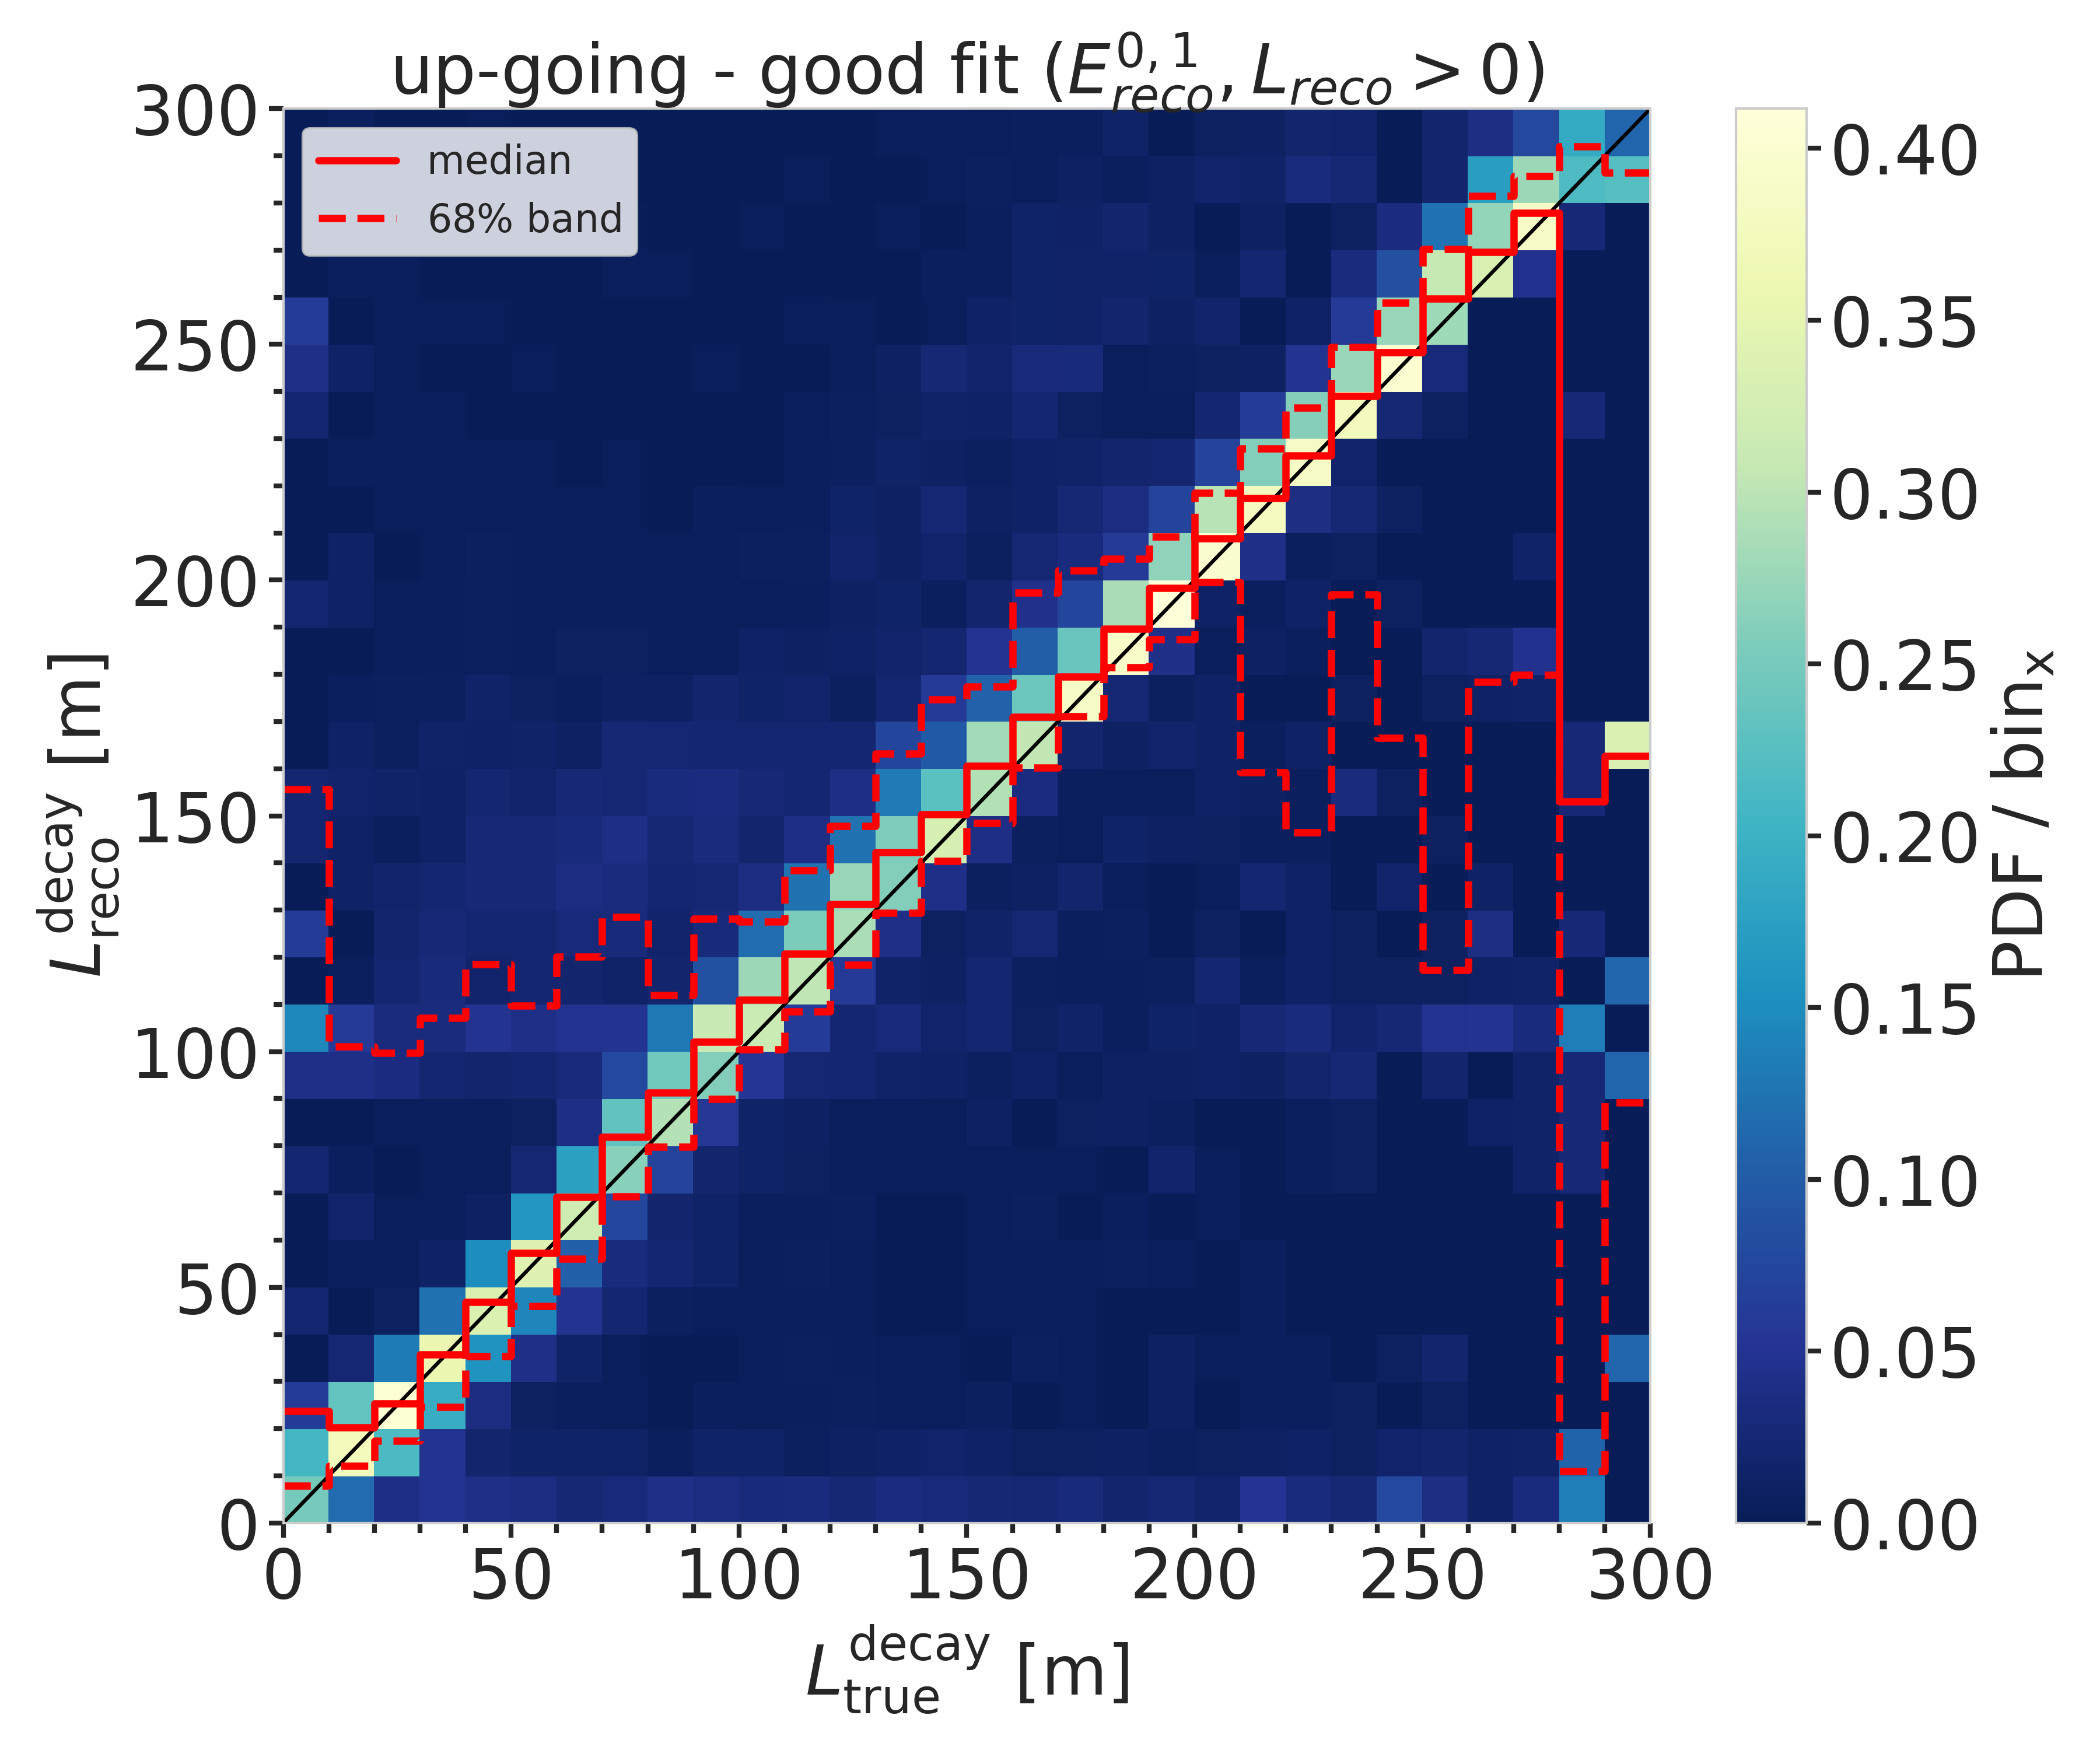
\includegraphics[width=0.49\linewidth]{figures/model_independent_simulation/results/idealistic/194601_reco_decay_length_vs_true_decay_length_goodfit_step_contours.png}
    \caption[]{}
    \labfig{idealistic_length_resolutions}
\end{figure*}
\todo{fix caption of this figure (RED)}

The two-dimensional histogram shows that there is no under-estimation of the length up to a true decay length of $\sim$\SI{210}{\meter}, which shows that if there are DOMs in the region between the two cascades that have not observed any light, the reconstruction is very stable. Considering the underlying Poisson likelihood in \refeq{millipede_likelihood} used for the reconstruction, this makes sense, since DOMs being present, but not observing any light is affecting the light expectation that goes into the likelihood and therefore makes these hypotheses unlikely and therefore incompatible with the data.


\subsection{Realistic Events}

The sample of HNL events introduced in \refsec{realistic_sample}, which is a more realistic representation of the expected HNL events, but still offers more controlled energy and length distributions, is used to investigate the selection efficiency, to cross check the reconstruction performance, and to benchmark the limits where the reconstruction breaks down. An example event view is shown in \reffig{realistic_example_event}, for cascade energies of \SI{30.8}{\gev} and \SI{25.3}{\gev}, and a decay length of \SI{144.5}{\meter}. Since the size of the colored spheres is proportional to the number of photons observed in the DOMs, it can be seen from the event view that even for these higher energies, only individual or few photons are observed. This makes detecting and reconstructing them significantly more challenging and is purely due to the larger distance of the cascades from the DOMs.

\begin{marginfigure}
    \centering
    % [trim=left bottom right top, clip]
    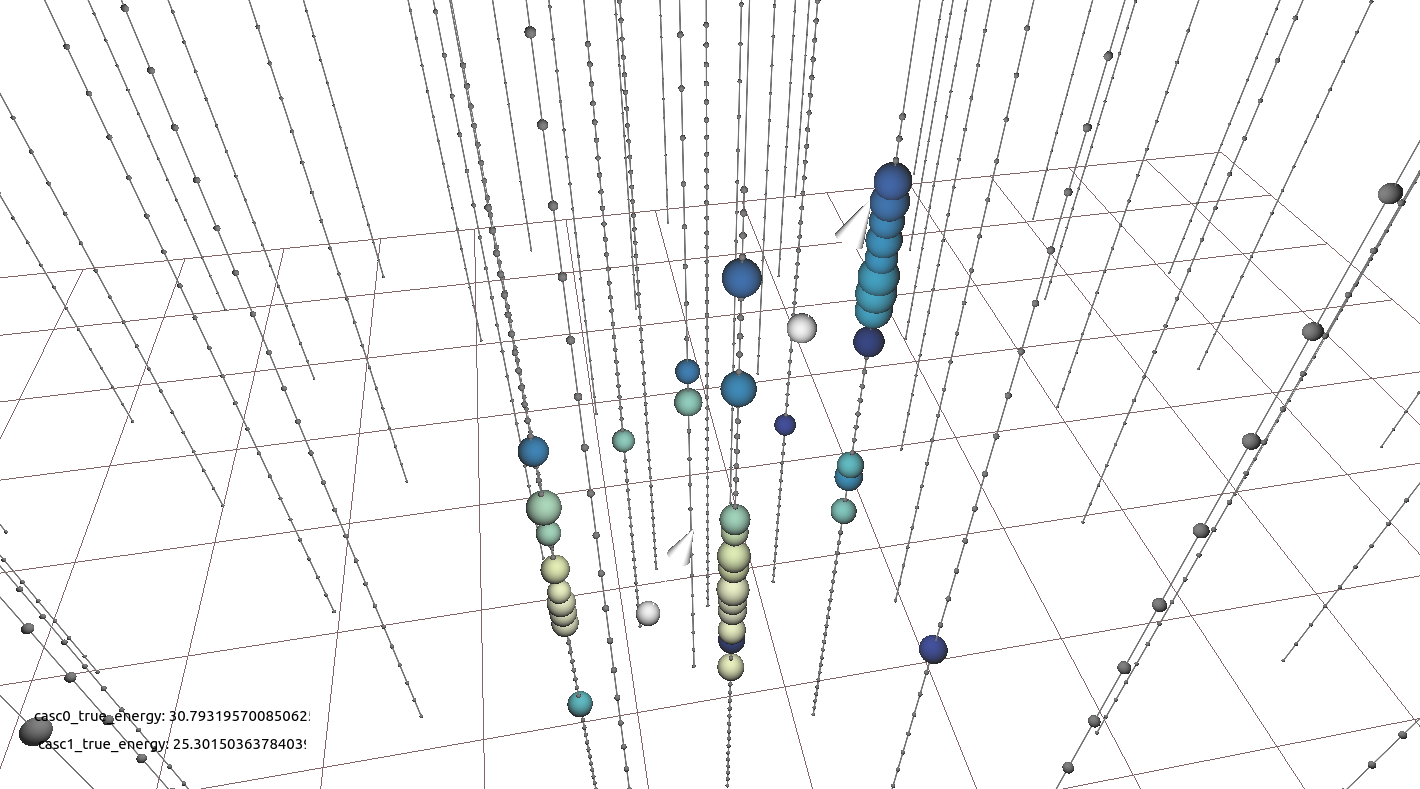
\includegraphics[trim=230 45 230 65, clip]{figures/model_independent_simulation/diagonal_e0_30.8_e1_25.3_v0.png}
    \caption[Event view of a realistic double cascade event]{Event view of a realistic double cascade event, with cascade energies of \SI{30.8}{\gev} and \SI{25.3}{\gev}, and a decay length of \SI{144.5}{\meter}. The colored spheres show the DOMs that have observed light, where the size is proportional to the number of observed photons and the color indicates the time (yellow is early, blue is late). The strings are shown as black lines, with small spheres indicating the DOM positions, and the true cascade vertices and directions are shown as white spheres with white arrows.}
    \labfig{realistic_example_event}
\end{marginfigure}

To assess the efficiency of the low energy event selection introduced in \refsec{processing_chain}, the energy and length distributions are shown across the different selection levels in \reffig{realistic_selection}\todo{Make/add relevant plots here (RED)}. \reftab{realistic_selection_efficiency} shows the total efficiency of the selection, where it can be seen that at level xx it is reduced the most and only xx\% of the events pass the selection to level 5.

\todo{Plot energy (true total) and true decay length across the different levels (RED)}
\todo{Make table with the rates across the different levels for benchmark mass/mixing (RED)}

The energy distributions in \reffig{cascade_energy_2dhists} show a similar behavior to the results discussed in \refsec{190607_energy_resolutions}. The difference is that now, there is no bias in the reconstructed energy, because the events are simulated as EM cascades, which means all energy is deposited in light and can be reconstructed. Above around \SIrange{5}{6}{\gev} the median is very stable, and the 1-sigma resolution band is \SI{50}{\percent} narrow and decreasing with energy down to \SI{20}{\percent} at \SI{100}{\gev}. Interestingly, the second cascade energy reconstruction performs slightly worse, although they have the same energy ranges for this sample. This could hint at an asymmetry in the reconstruction process, which might relate to how the two cascades are parameterized, or be due to the different positions and the dominantly up-going direction used in the sampling combined with the DOMs looking down. The total energy resolution shown in the left part of \reffig{total_energy_decay_length_2dhists} is very good, above \SI{10}{\gev} it is unbiased and the 1-sigma resolution band is below \SI{20}{\percent}.

\begin{figure*}[h]
    \centering
    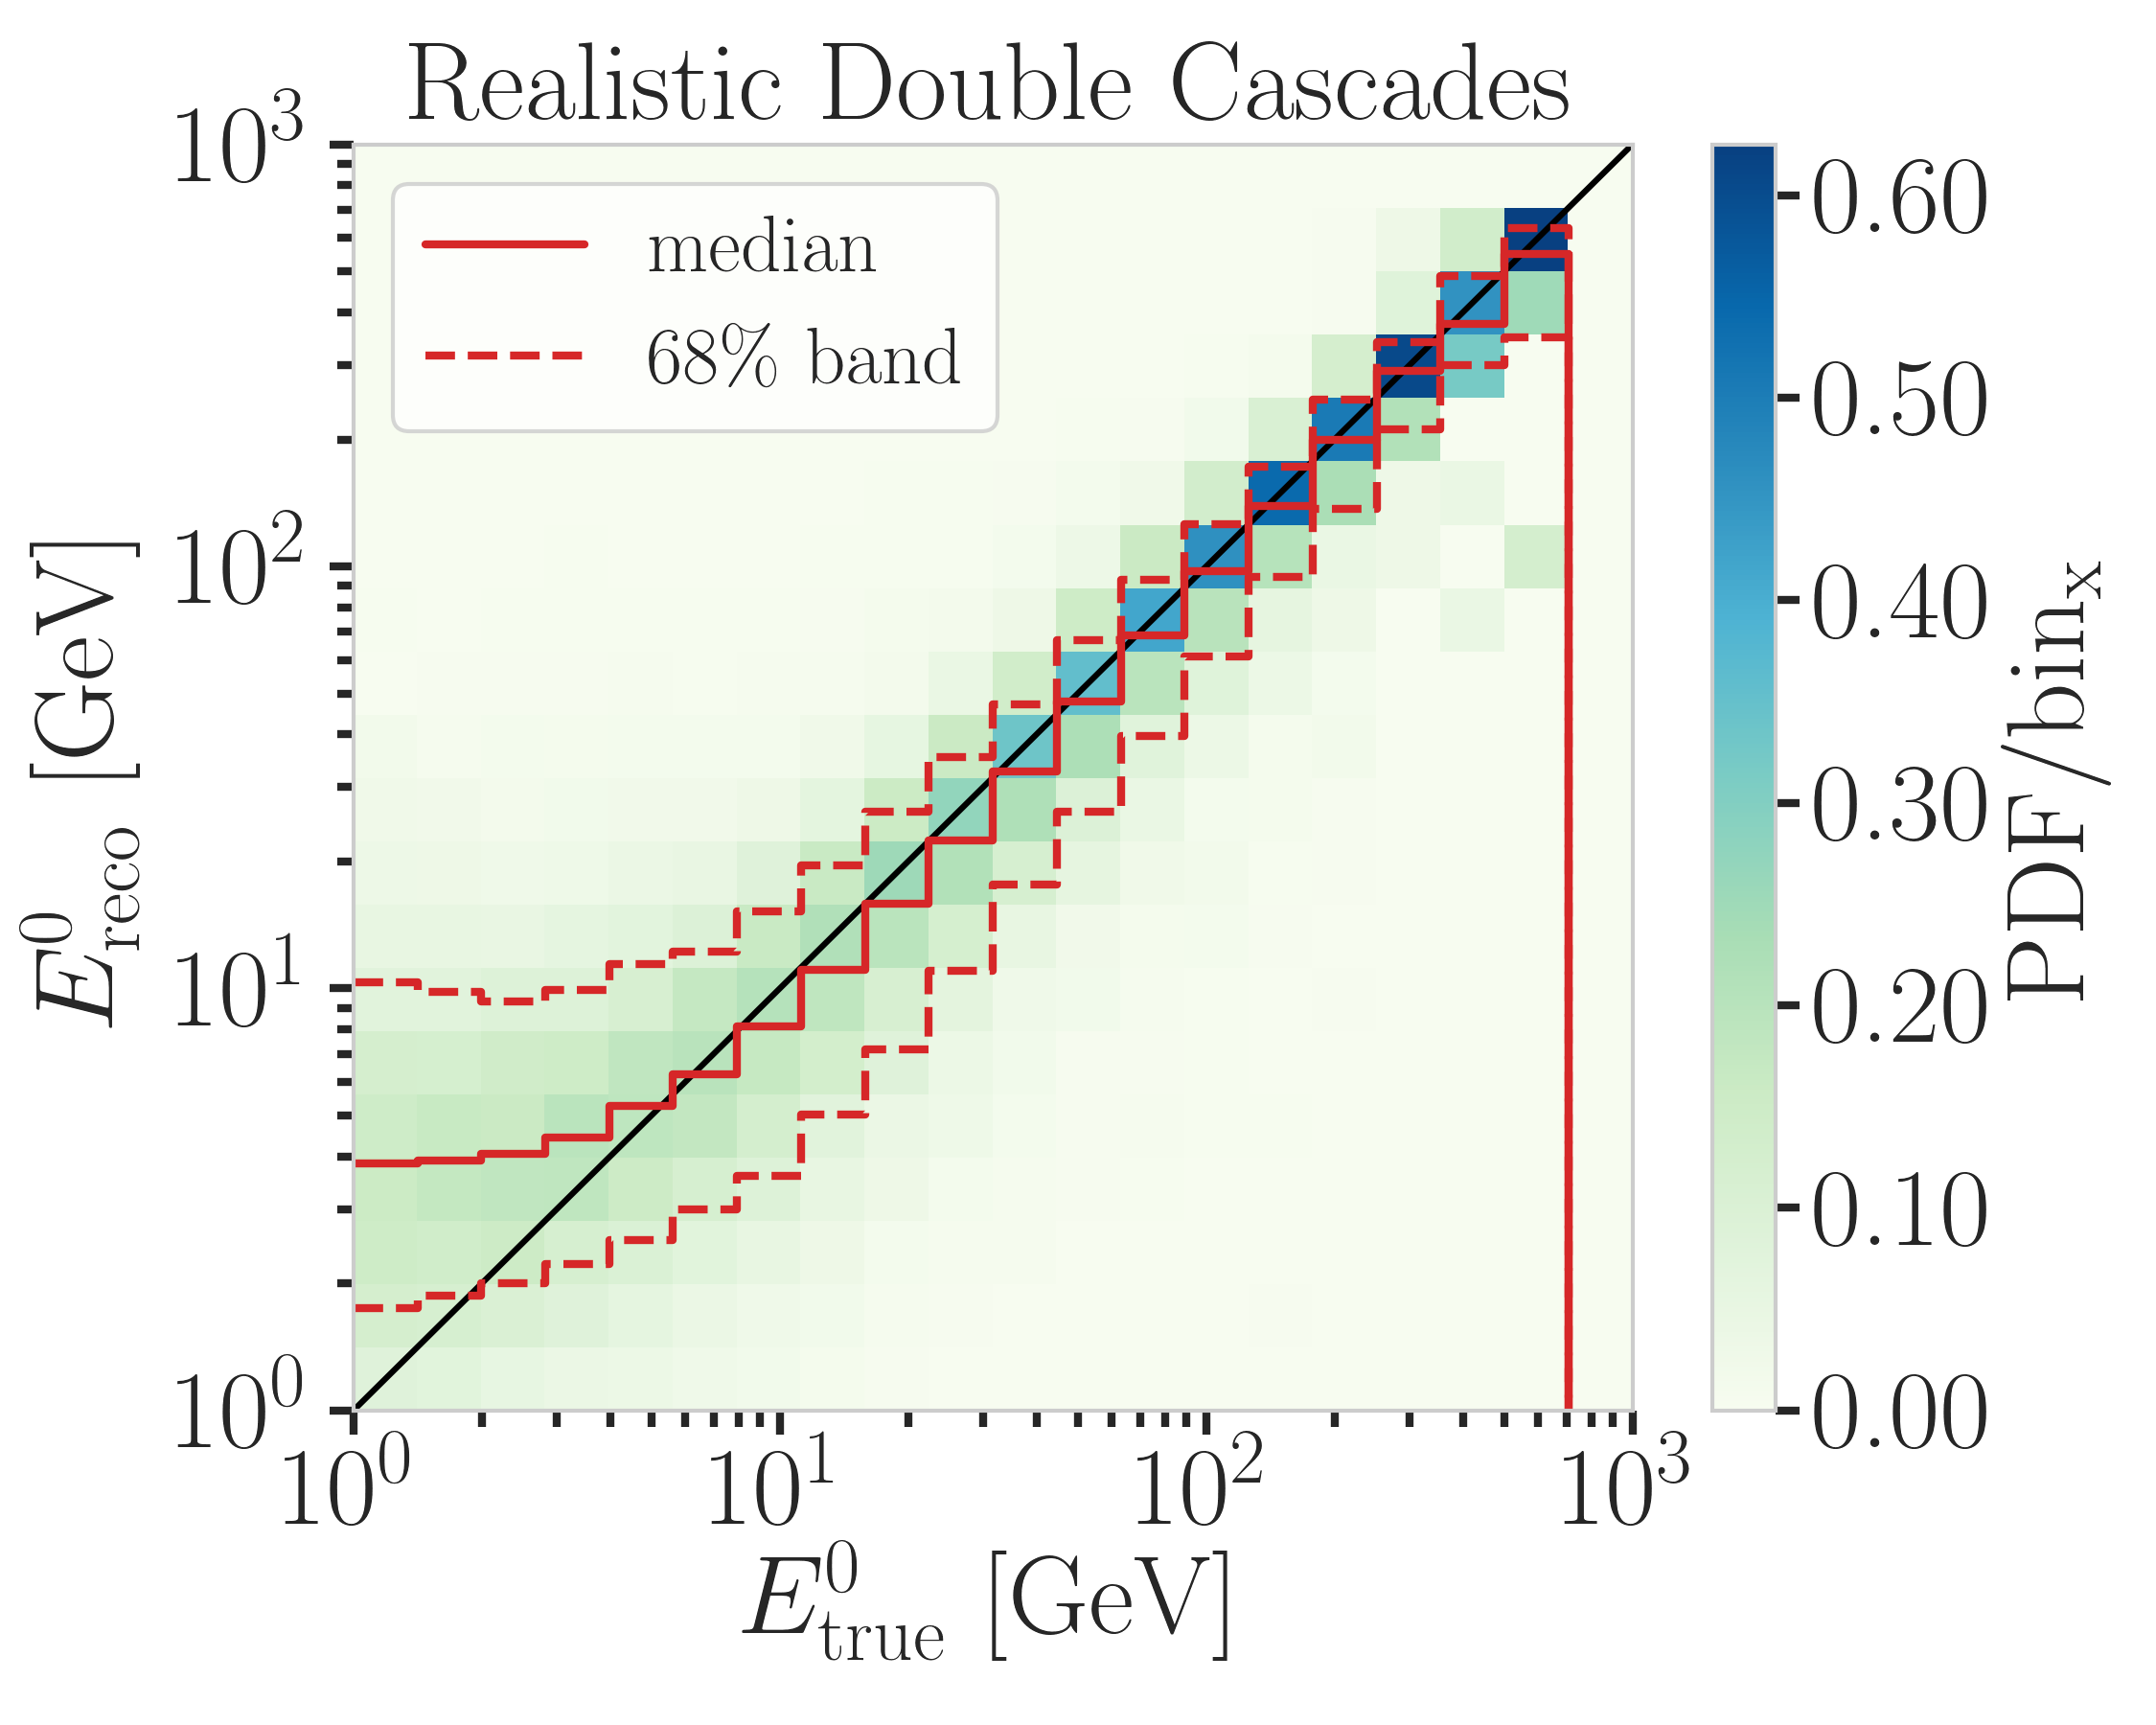
\includegraphics[width=0.49\linewidth]{figures/model_independent_simulation/results/realistic/2d_hists/194603_casc0_reco_energy_vs_casc0_true_energy_goodfit_step_contours.png}
    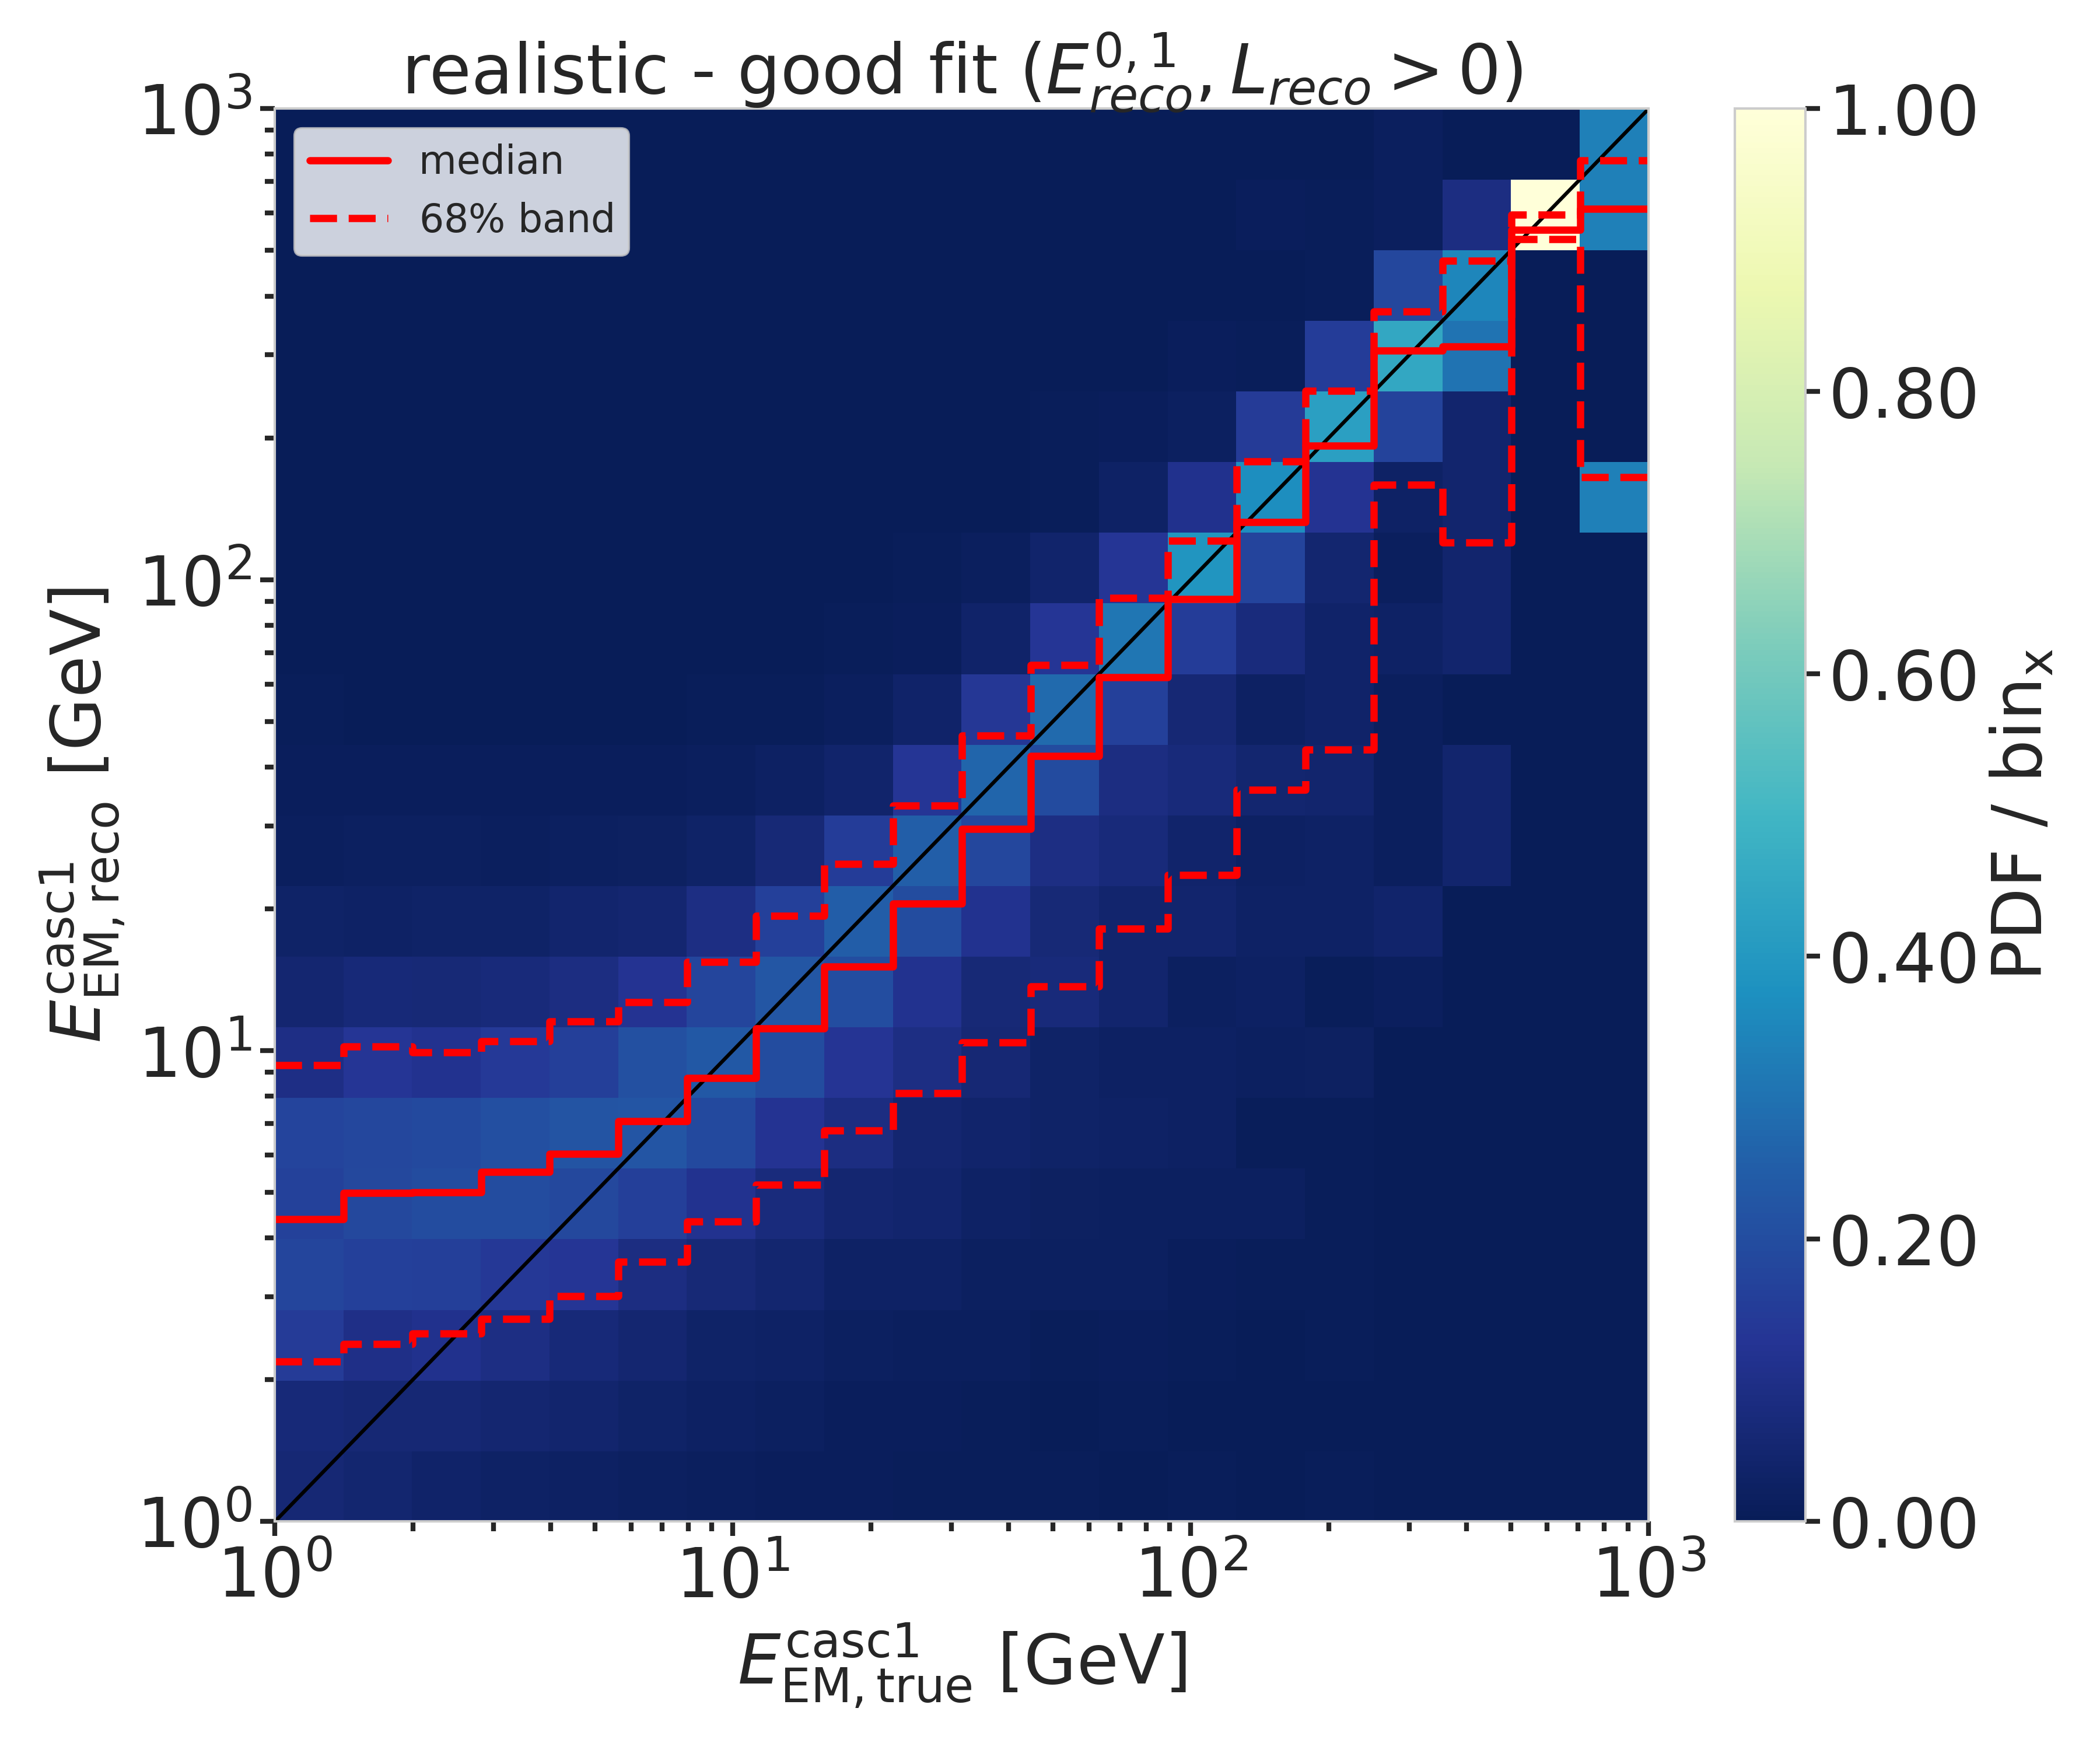
\includegraphics[width=0.49\linewidth]{figures/model_independent_simulation/results/realistic/2d_hists/194603_casc1_reco_energy_vs_casc1_true_energy_goodfit_step_contours.png}
    \caption[]{}
    \labfig{cascade_energy_2dhists}
\end{figure*}
\todo{fix caption of this figure (RED)}

The decay length resolution shown in the right part of \reffig{total_energy_decay_length_2dhists} looks similarly bad to the results discussed in \refsec{190607_length_resolutions} and shows the same features with a region between \SIrange[range-phrase={~and~}]{20}{80}{\meter} where it is roughly unbiased, but the 1-sigma resolution band is wide with a lot of outliers towards short reconstructed lengths. Below \SI{65.8}{\meter} the reconstructed lengths are always over-estimating the true and above \SI{80}{\meter} a population of events start to dominate where the decay lengths is not getting reconstructed at all, as investigated before.

\begin{figure*}[h]
	\centering
    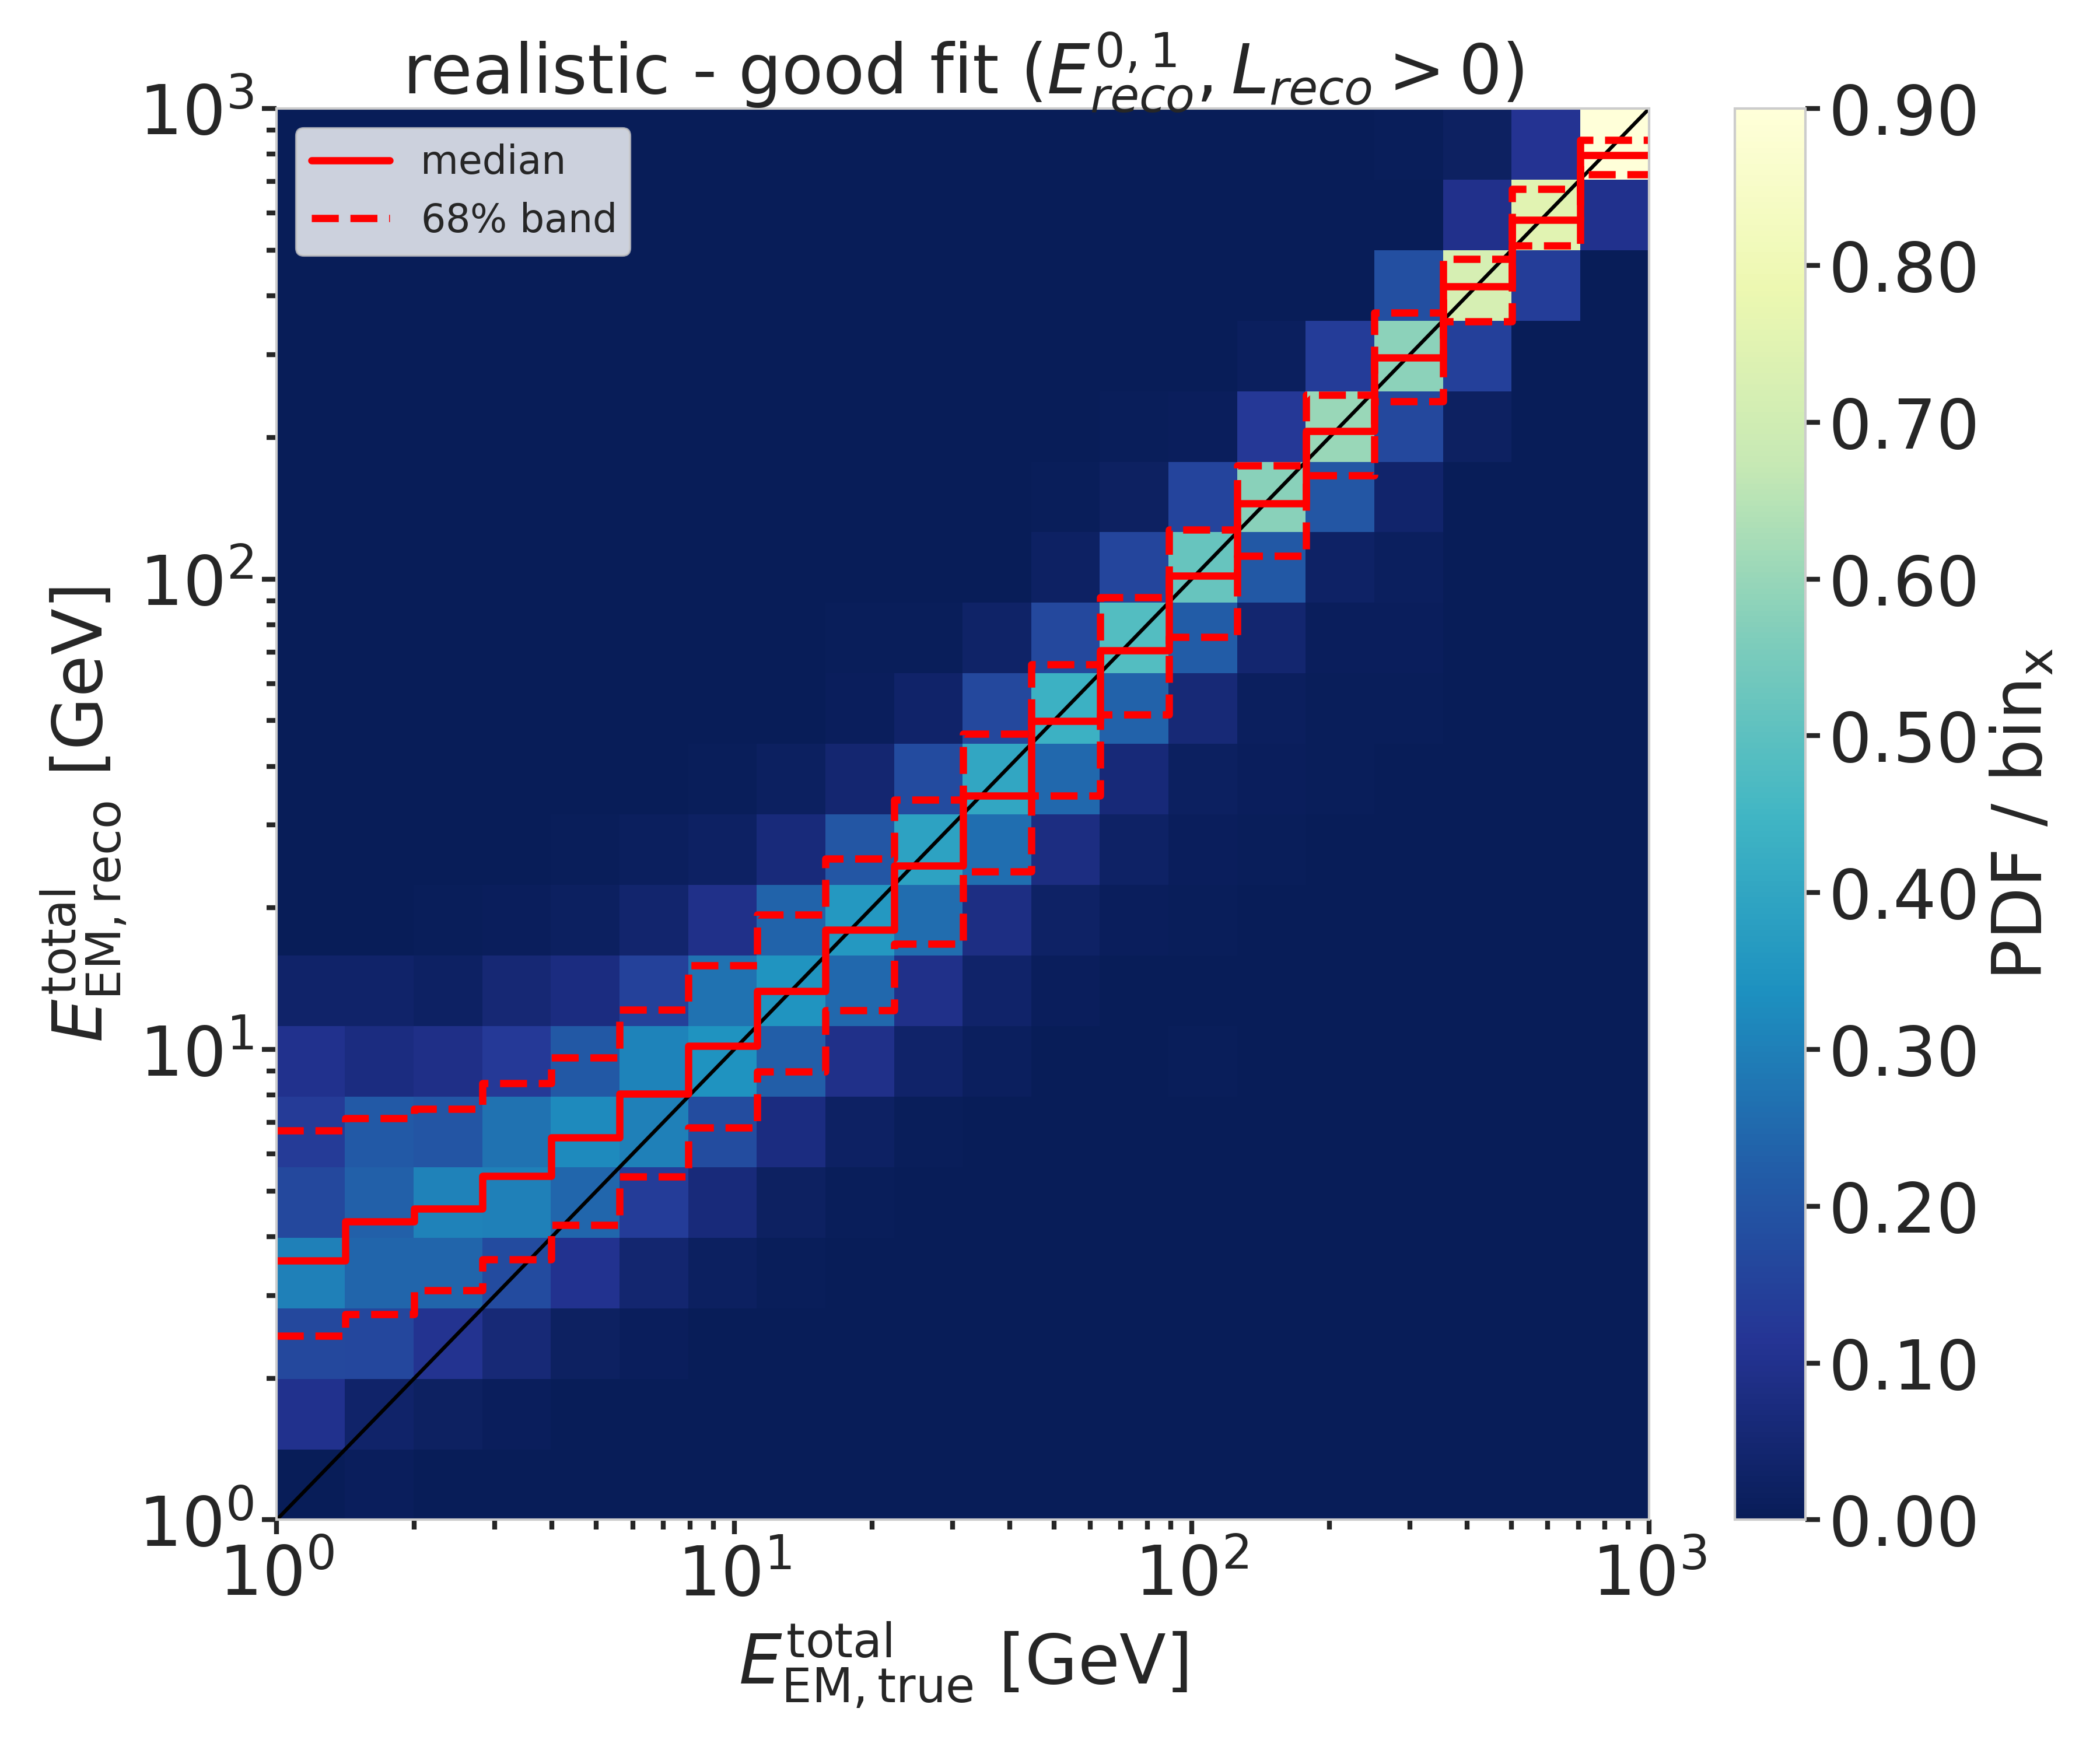
\includegraphics[width=0.49\linewidth]{figures/model_independent_simulation/results/realistic/2d_hists/194603_reco_total_energy_vs_true_total_energy_goodfit_step_contours.png}
    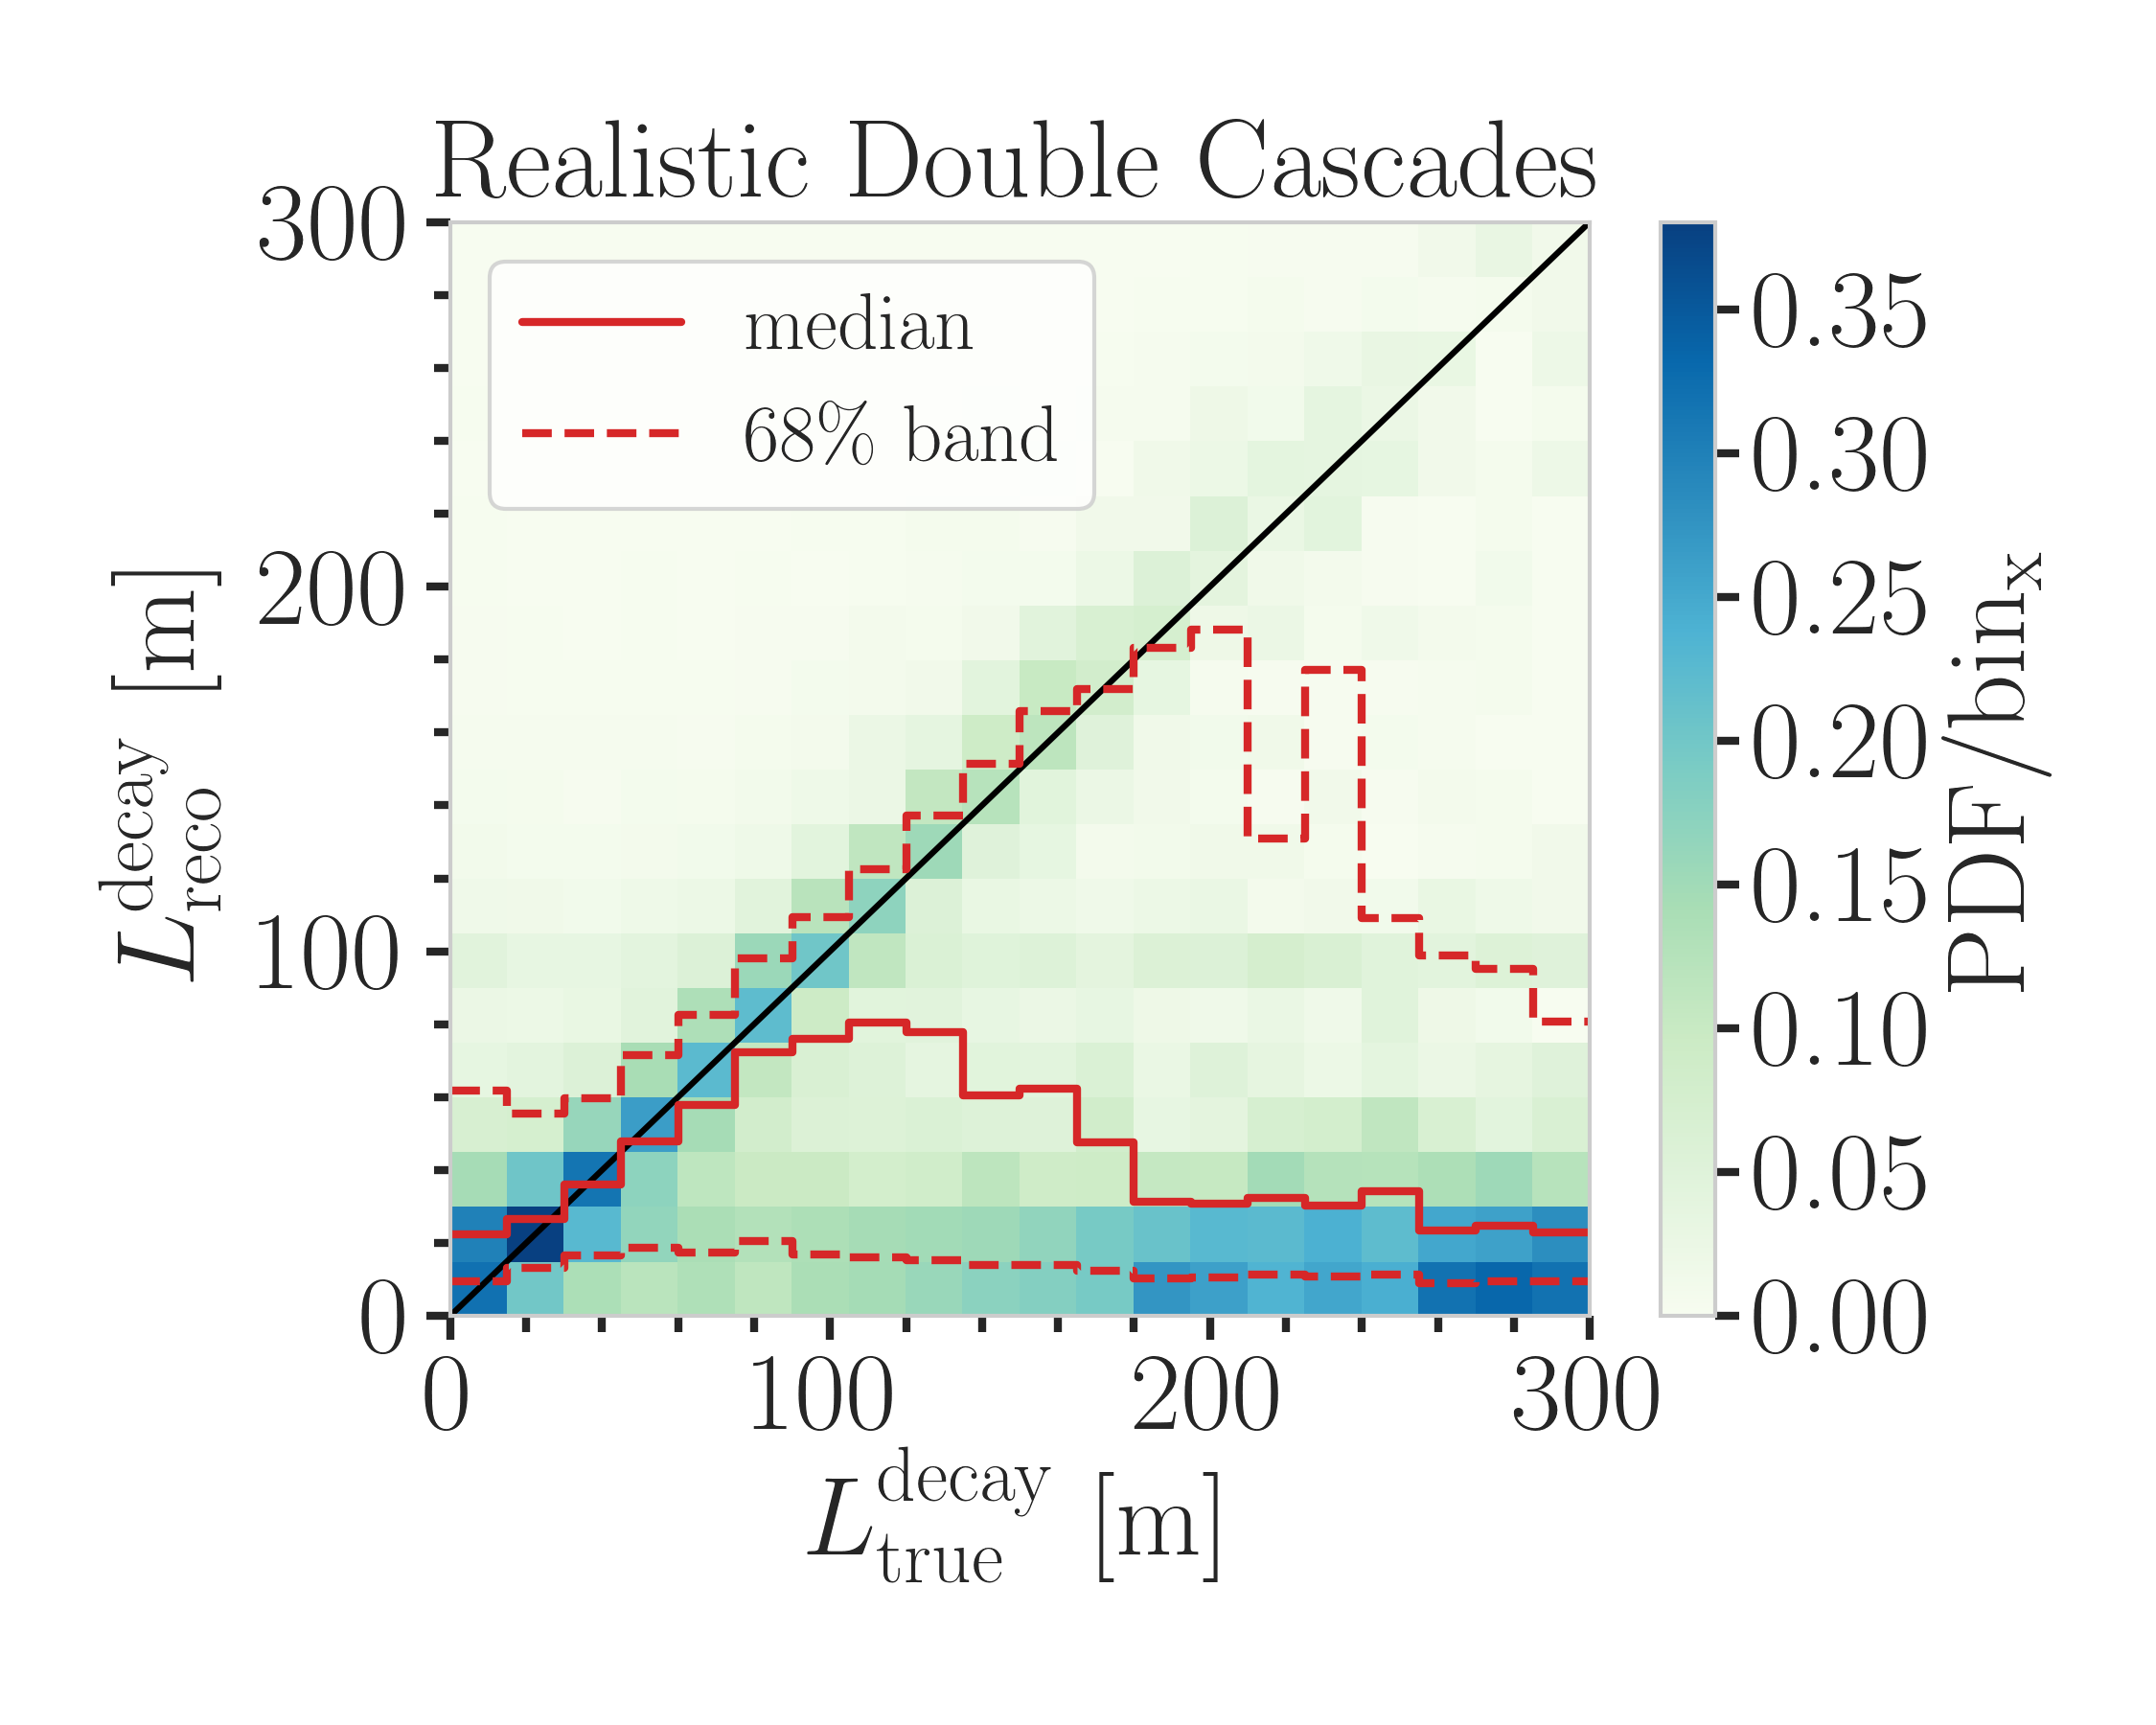
\includegraphics[width=0.49\linewidth]{figures/model_independent_simulation/results/realistic/2d_hists/194603_reco_decay_length_vs_true_decay_length_goodfit_step_contours.png}
    \caption[]{}
    \labfig{total_energy_decay_length_2dhists}
\end{figure*}
\todo{fix caption of this figure (RED)}

To get an estimate of what minimum energies are necessary for the reconstruction to perform reasonably well, the fractional decay length resolution is shown as a function of the total true energy and the minimum energy of both individual cascades in \reffig{decay_length_bias_vs_energies}. In the left part it can be seen that the median of the decay length resolution stabilizes around 0 for a total energy above \SI{20}{\gev}, but the spread of the distribution is still quite large with a 1-sigma band of \SIrange{80}{100}{\percent}, decreasing down to $\sim$\SI{60}{\percent} at \SI{100}{\gev}. Based on the right part of the figure, the decay length resolution starts to be unbiased for a minimum energy of any cascade of \SI{7}{\gev}, with an equivalently large spread. A rough takeaway from this is that the decay length reconstruction is not reliable for events with one cascade energy below \SI{7}{\gev} and with a total energy below \SI{20}{\gev}. Above these values the median resolution is roughly unbiased, but the spread is still large, decreasing with increasing energy.

\begin{figure*}[h]
	\centering
    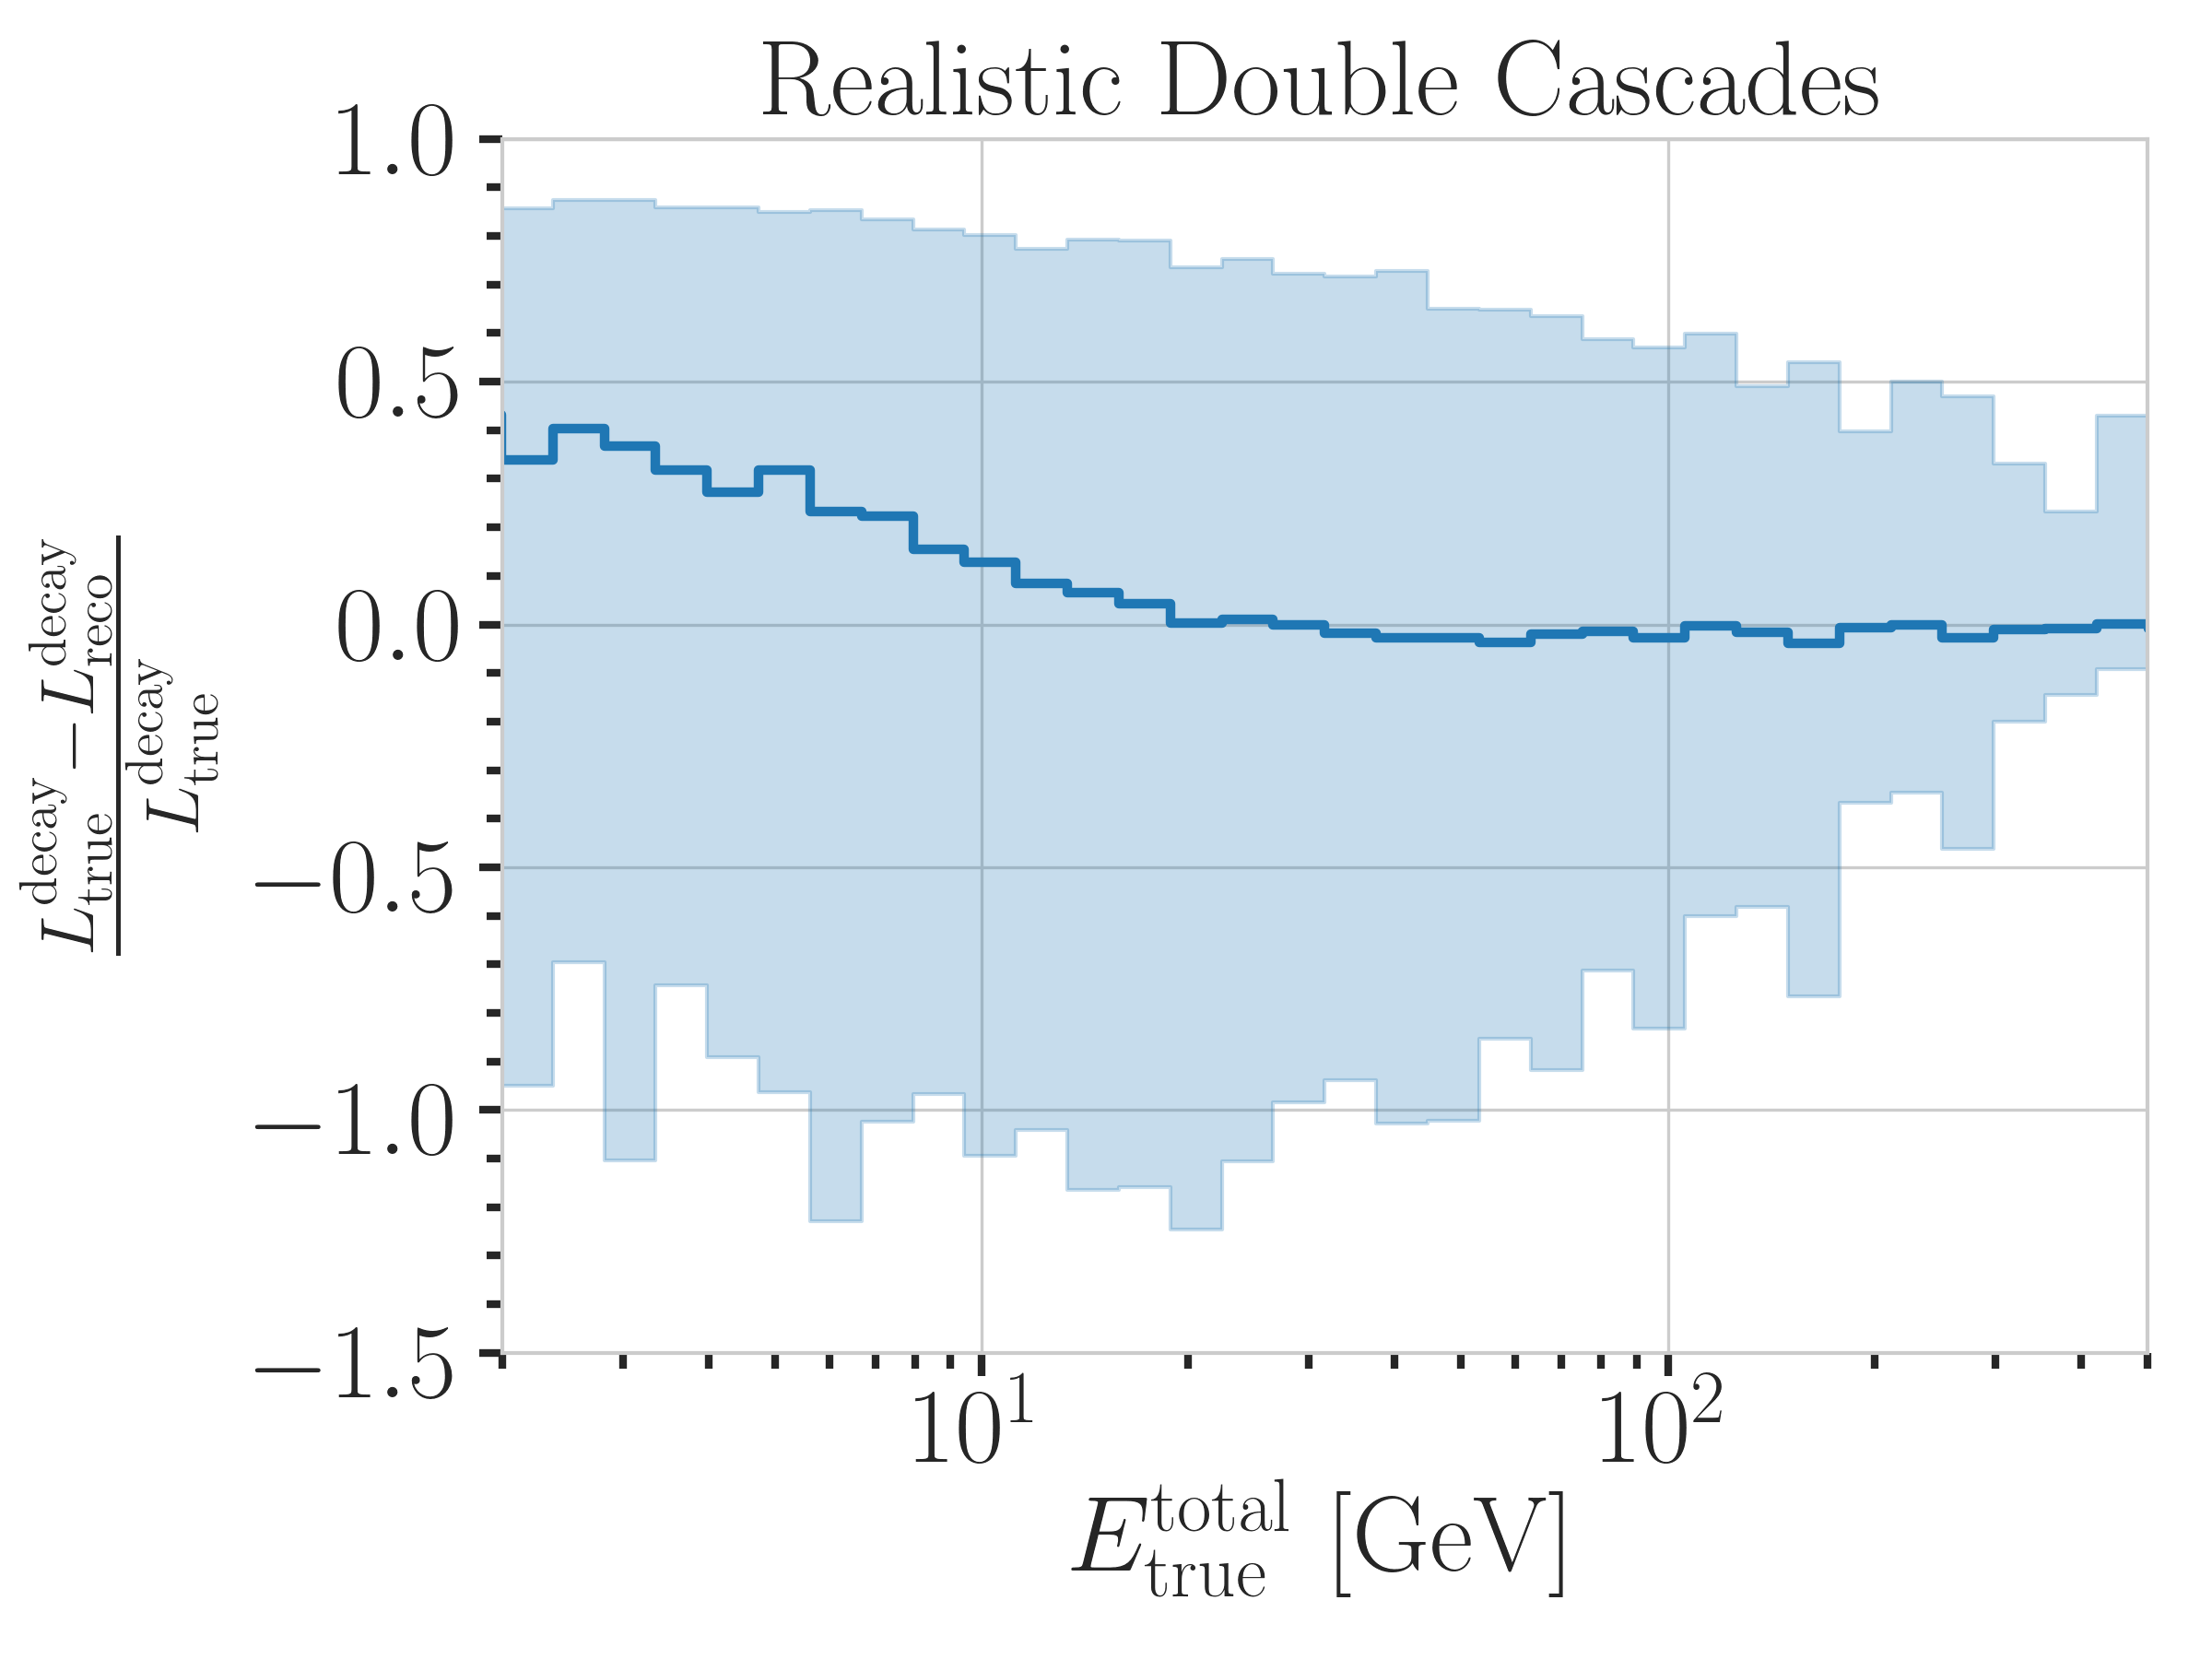
\includegraphics[width=0.49\linewidth]{figures/model_independent_simulation/results/realistic/resolutions/194603_median_decay_length_bias_vs_tot_energy_goodfit_log_unweighted.png}
    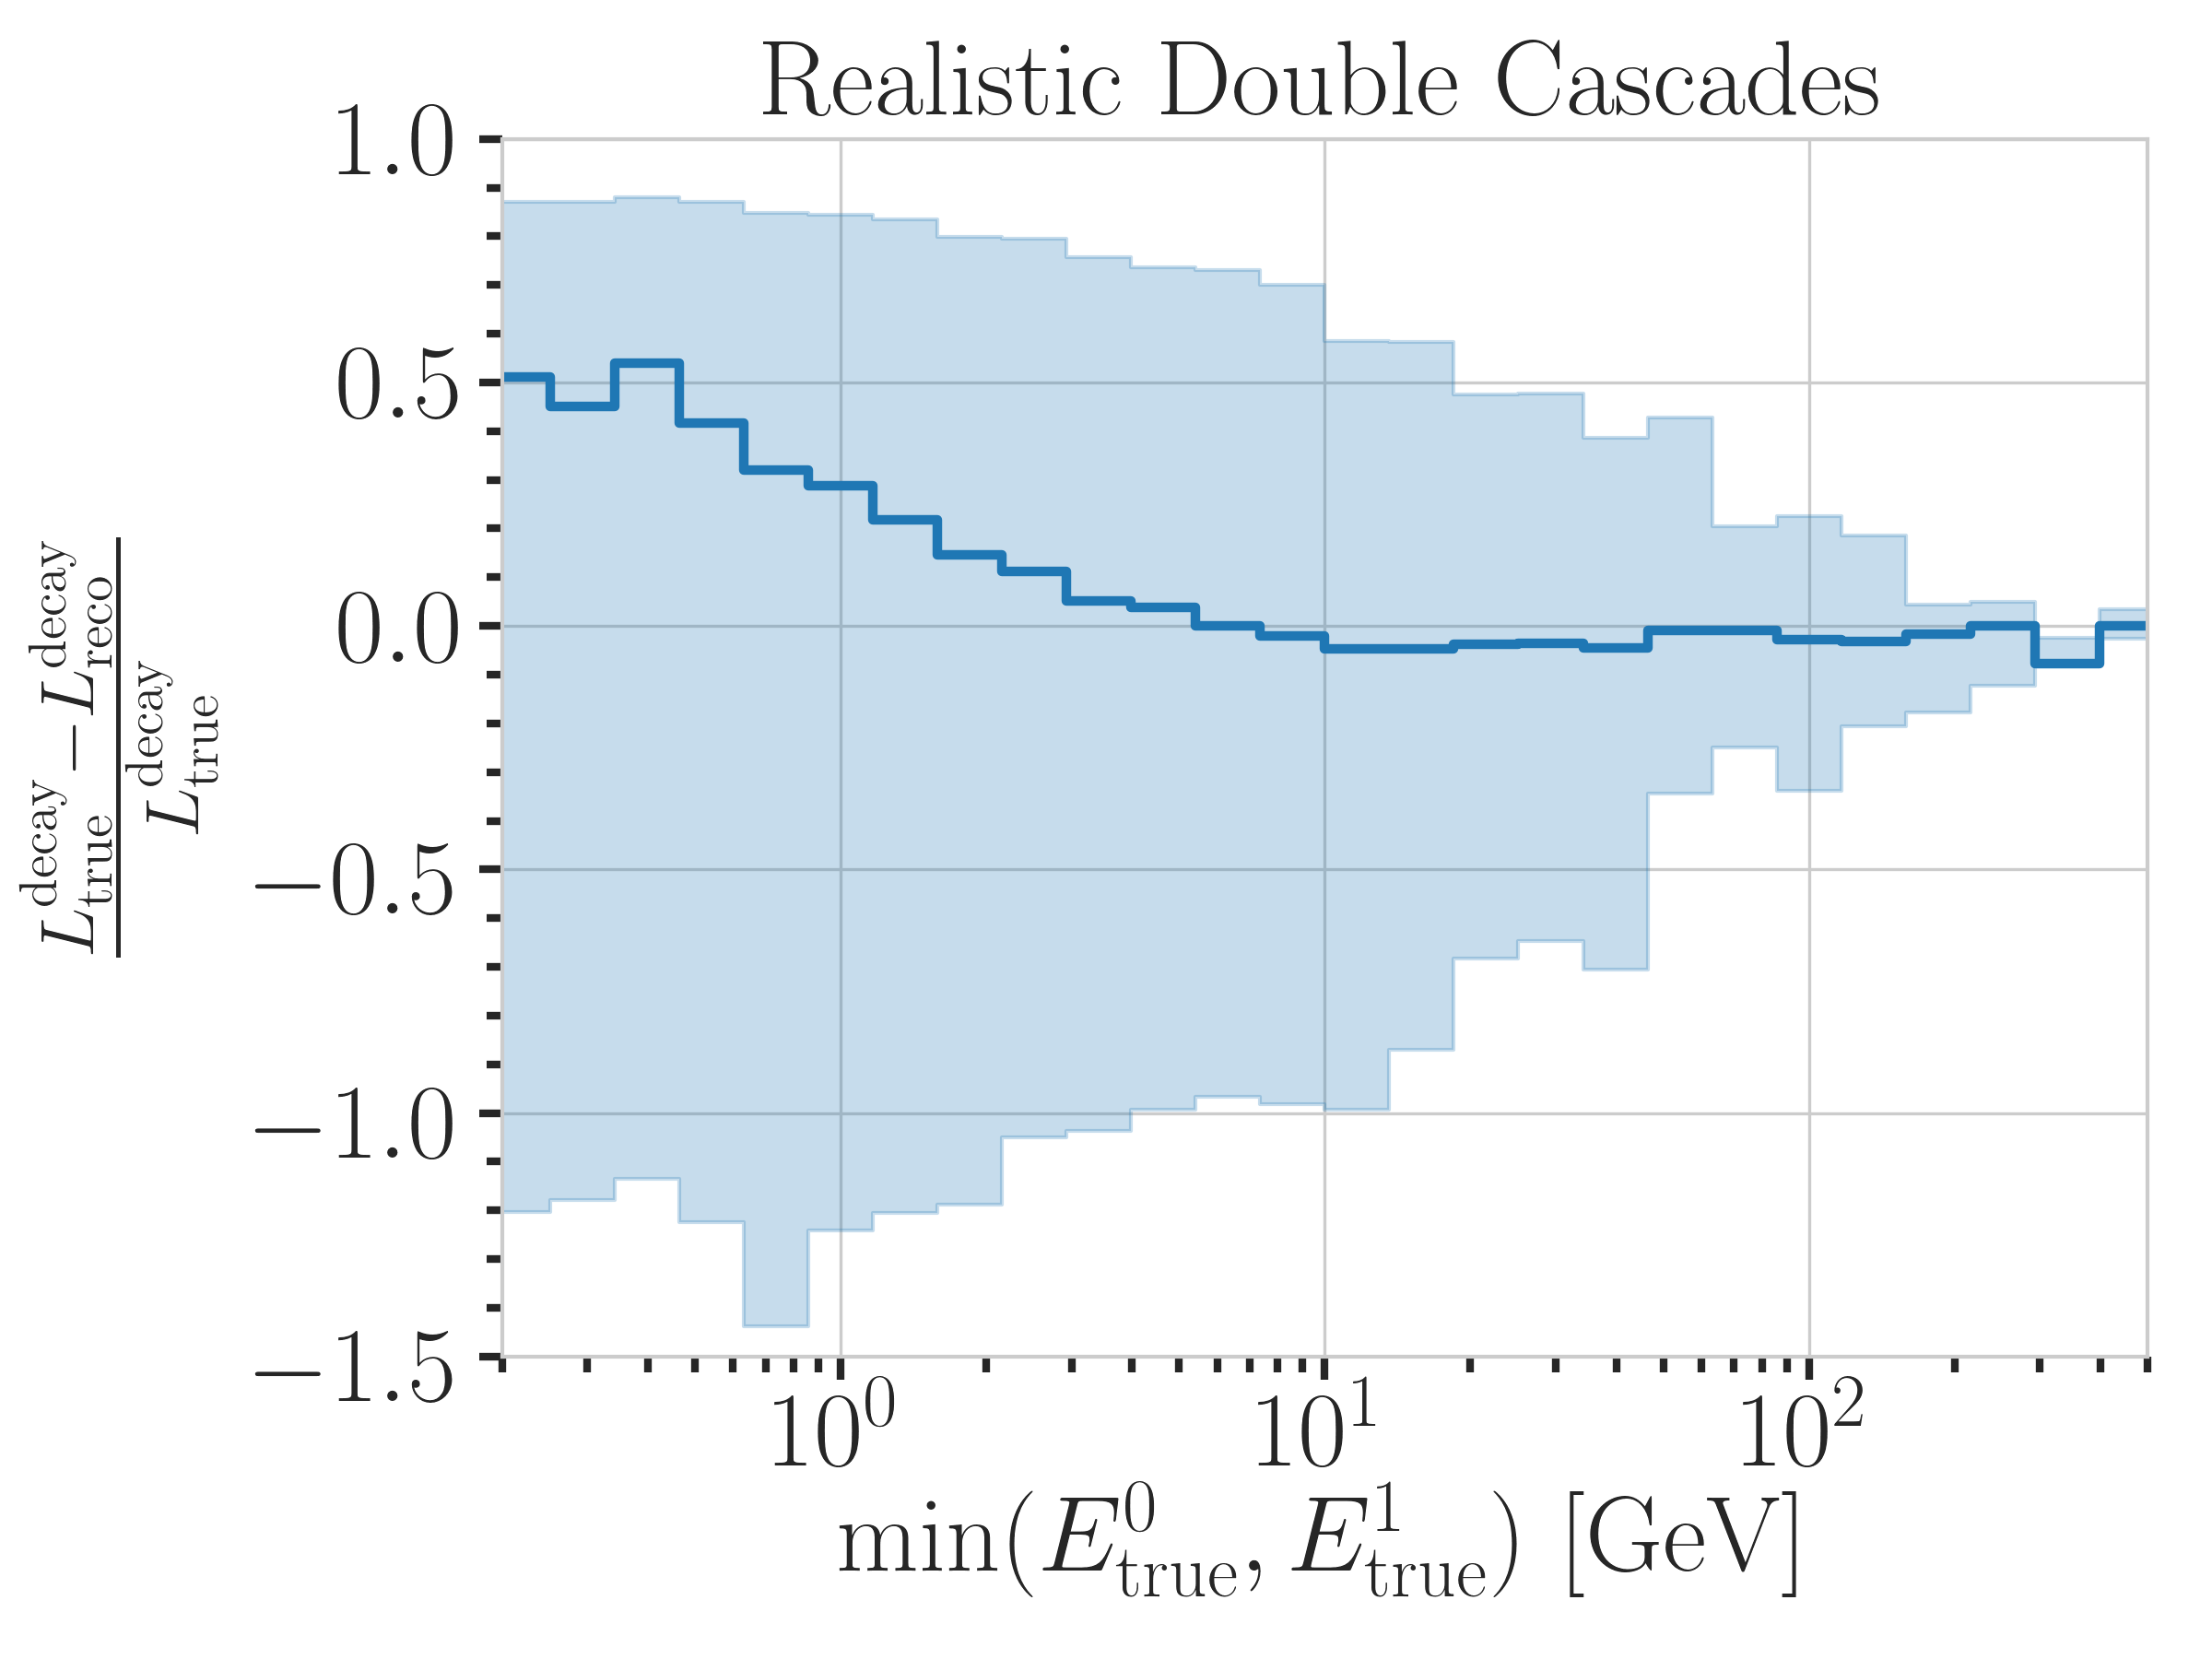
\includegraphics[width=0.49\linewidth]{figures/model_independent_simulation/results/realistic/resolutions/194603_median_decay_length_bias_vs_min_energy_goodfit_log_unweighted.png} 
    \caption[]{}
    \labfig{decay_length_bias_vs_energies}
\end{figure*}
\todo{fix caption of this figure (RED)}


\section{Summary and Outlook}

\todo{write summary and outlook (RED)}

From the investigation of the good and badly reconstructed events, it can be concluded that the main reason for the bad reconstruction is the low energy of the second cascade. Despite the fact that the split into the two populations was very rudimentary, it is clear that this is the dominant cause, while other factors, like the position of the second cascade, or the potentially bad input seed direction are also contributing. For a thorough investigation, a more sophisticated separation would be needed.


- upgrade?
- other selection?
- other reconstruction?
